\documentclass[runningheads]{llncs}

\usepackage[T1]{fontenc}
\usepackage[utf8]{inputenc}
\usepackage[numbers,sort&compress]{natbib}
\usepackage{hyperref}
\usepackage{url}
\usepackage{booktabs}
\usepackage{amsfonts}
\usepackage{amsmath}
\usepackage{amssymb}
\usepackage{nicefrac}
\usepackage{microtype}
\usepackage{xcolor}
\usepackage{multirow}
\usepackage{graphicx}
\graphicspath{{./}{../}}
\usepackage{enumitem}

\begin{document}

\title{Expected Free Energy as Belief-Dependent Utility for $\rho$-POMDPs:\\
From a Canonical Information-Unit Weight to an Operational Shadow Price}

\titlerunning{EFE for $\rho$-POMDPs: Canonical Weight to Operational Shadow Price}

\author{Patrick Cooper \and Alvaro Velasquez}

\authorrunning{P. Cooper and A. Velasquez}

\institute{Department of Computer Science, University of Colorado Boulder,\\ Boulder, CO, USA\\
\email{\{patrick.cooper,alvaro.velasquez\}@colorado.edu}}

\maketitle

\begin{abstract}
An agent acting under partial observability must decide how much effort to spend gathering information before committing to a decision, and standard POMDPs give it no direct way to state that spending limit: information has value only through its downstream effect on reward. We address this by treating information acquisition in a $\rho$-POMDP (a POMDP extended with a belief-dependent utility $\rho$) as an explicitly budgeted resource. Given a stated sensing budget $B$, how much observation the agent may use before committing, the weight to place on an information-gain utility is the budget's operational shadow price $w^*(B)$, the weight at which the agent's induced sensing usage meets $B$: a value computable offline from a usage curve, trackable online by dual descent when the reward scale itself shifts mid-run, and exactly scale equivariant for the implemented agent, so it need not be re-tuned when rewards are rescaled. This budgeted formulation rests on an exact theoretical identification: minimizing Expected Free Energy (EFE) under active inference is provably equivalent to solving a $\rho$-POMDP whose utility is expected information gain at the canonical weight $w{=}1$, exact under log scoring rules \citep{bernardo1979}, for observe-then-commit POMDPs and, for the hidden-state-preserving observation and navigation actions that gather information, for factored observation POMDPs covering interleaved observe-act problems such as non-destructive testing and mobile sensing. The canonical weight $w{=}1$ is recovered as the special case of the budgeted formulation that buys whatever sensing the ambient reward scale happens to imply, making it a derived default under a shared reward convention rather than a universal, scale-invariant calibration. Across environments ranging from the classic Tiger problem through RockSample to a Structural Inspection benchmark with over $65{,}000$ states, this default sits near the reward-maximizing knee of the success--reward Pareto frontier and matches a near-optimal SARSOP reference within sampling error on the three core observe-then-commit environments. The budgeted formulation further gives a set-valued price at usage gaps rather than a misleading point estimate, reducing the practical design question from ``what should the information weight be'' to ``how much sensing can we afford.''
\keywords{Active inference \and Expected free energy \and $\rho$-POMDPs \and Epistemic value \and Belief-dependent utility \and Partial observability \and Information gain \and Sensing budgets \and Shadow prices}
\end{abstract}

\section{Introduction}

Decision-making under partial observability requires agents to balance exploiting current knowledge against gathering information to reduce uncertainty about hidden states. In standard POMDPs, information gathering has no intrinsic value. It is useful only insofar as it leads to higher expected reward. This creates a well-known difficulty: the exploration--exploitation trade-off must be resolved either by the planning horizon or by heuristic exploration bonuses.

The $\rho$-POMDP framework \citep{araya2010} addresses this by extending POMDPs with a belief-dependent utility $\rho(b)$ that allows the agent to derive value directly from properties of its belief state. This enables explicit optimization over uncertainty reduction, information gain, or other belief-state properties alongside task reward. However, the choice of $\rho$ remains largely heuristic and environment-specific, and, when $\rho$ is an information-gain term, so does the weight placed on it.

This paper treats that weight as a design problem with a resource-allocation answer. State a sensing budget $B$, the amount of observation the agent may use before committing, and price the information-gain utility at the budget's \emph{operational shadow price} $w^*(B)$: the weight at which the agent chooses to spend about $B$ on sensing. That price is computable offline from a usage curve relating weight to expected sensing usage (Section~\ref{sec:budget}), trackable online by dual descent -- with stationary convergence guaranteed (Proposition~\ref{prop:pi5}) and re-adaptation under mid-run reward-scale shift demonstrated empirically (Section~\ref{sec:dual_multiseed}) -- exactly scale equivariant for the implemented agent so it need not be re-tuned when rewards are rescaled (Proposition~\ref{prop:pi1}), and set-valued, a bracket rather than a point, whenever the budget falls at a usage gap (Definition~\ref{def:pi3}). The question ``what weight should the information-gain utility carry'' becomes ``how much sensing can we afford,'' with the weight read off the stated budget rather than searched per task.

The active inference (AIF) framework \citep{friston2010, parr2019} identifies one canonical point on this price curve. AIF casts perception and action as approximate Bayesian inference, selecting policies that minimize Expected Free Energy (EFE). EFE naturally decomposes into a pragmatic term (goal-seeking) and an epistemic term (information-seeking). Because both terms come from a single variational objective, their relative coefficient is fixed once pragmatic value is identified with task reward. In the discrete-state formulation we use, that coefficient is $w{=}1$ in information units (Proposition~\ref{prop:equivalence}). The claim is exact under log scoring rules \citep{bernardo1979} and, under a shared reward convention, an empirically robust untuned default. It is not scale-invariant: multiplying every reward and cost by $\alpha>0$ leaves the bit-valued information term unchanged, so a fixed $w{=}1$ implements a different trade-off at every scale. Rather than treating this as a limitation to caveat, we read it as confirmation that $w$ is a price: $w{=}1$ is recovered as exactly the special case of the budgeted formulation above that buys whatever sensing the ambient reward scale happens to imply, not a universal, scale-invariant calibration.

We propose substituting EFE as $\rho$ in $\rho$-POMDPs, yielding an agent whose epistemic foraging is a consequence of its objective rather than an engineered bonus.\footnote{Code and experiment data are available at \url{https://github.com/PatrickAllenCooper/rho_aif}.} Our contributions are:
\begin{enumerate}
    \item Theory. A formal bridge between $\rho$-POMDPs and active inference. We prove the equivalence for observe-then-commit POMDPs (Proposition~\ref{prop:equivalence}), characterize when the information-unit weight $w{=}1$ is near-optimal (Proposition~\ref{prop:nearopt}), and extend the equivalence to factored observation POMDPs, interleaved settings where information gathering preserves the hidden state (Proposition~\ref{prop:factored}).
    \item Budgeted reformulation. We recast the information-unit weight as the operational shadow price $w^*(B)$ of a sensing budget $B$ (Section~\ref{sec:budget}), prove exact scale equivariance of the resulting policy family for the implemented receding-horizon agent (Proposition~\ref{prop:pi1}), define a set-valued price at usage gaps (Definition~\ref{def:pi3}), and give an online dual controller with a stationary convergence guarantee (Proposition~\ref{prop:pi5}) whose constant-step variant re-adapts empirically under reward-scale shift (Section~\ref{sec:dual_multiseed}).
    \item Evidence. Controlled comparisons against same-horizon planning, tuned information gain, and POMCP \citep{silver2010} across six observe-then-commit environments and four instances of the standard RockSample benchmark \citep{smith2004}. A Pareto analysis shows that on Diagnosis and Bandit, $w{=}1$ Pareto-dominates same-horizon planning, while remaining competitive with tuned Planning+IG across environments. A second experiment battery (Section~\ref{sec:budget_experiments}) shows usage-curve collapse across reward scales, closed-form onset thresholds recovered as the first knot of the usage staircase, multi-seed online tracking through a $\times 10$ reward rescale, and a near-optimal SARSOP reference matching EFE ($w{=}1$) within sampling error on the three core OTC environments.
    \item Practical guidance. A characterization of when EFE-as-$\rho$ helps and when it does not. The advantage appears when the agent must choose among multiple observation actions, and it grows with state space size ($69.4\%$ vs.\ $1.4\%$ success on Tileworld $8{\times}8$). On RockSample, the advantage is largest with several rocks to check ($+9.54$ reward over reward-only Planning on RockSample[7,8], $K{=}8$) but does not persist to every instance we test, vanishing on RockSample[11,11] ($K{=}11$) where both agents converge to the same saturated policy (Section~\ref{sec:rocksample}). We also report where it does not help by construction: ordinary information gain is reward-blind and will spend a sensing budget on task-irrelevant uncertainty (Section~\ref{sec:distractor}), and naive information gain can misvalue an action outright when observing changes the hidden state (Example~\ref{ex:destructive}).
\end{enumerate}

An abridged version of the equivalence results in Contribution~1 above, the observe-then-commit equivalence of Proposition~\ref{prop:equivalence}, the near-optimality characterization of Proposition~\ref{prop:nearopt}, the factored-observation extension of Proposition~\ref{prop:factored}, and the first experiment battery of Contribution~3, was accepted as a poster and spotlight presentation at the 7th International Workshop on Active Inference (IWAI 2026) \citep{cooper2026iwai}. This article is a substantially extended version. The entire budgeted $\rho$-POMDP formulation of Section~\ref{sec:budget} (Definition~\ref{def:pi3} and Propositions~\ref{prop:pi1}, \ref{prop:pi2}, \ref{prop:pi5}, and Corollary~\ref{cor:pi4}), the second experiment battery of Section~\ref{sec:budget_experiments}, and the practical guidance of Contribution~4 are new material that was not part of the IWAI submission.

\section{Related work}

\paragraph{POMDPs and solvers.}
POMDPs formalize sequential decision-making under state uncertainty \citep{smallwood1973, kaelbling1998}. Exact finite-horizon POMDP planning is PSPACE-complete. Point-based offline methods (PBVI \citep{pineau2003}, HSVI \citep{smith2004}, SARSOP \citep{kurniawati2008}) approximate the value function on reachable beliefs \citep{shani2013}. Online solvers plan from the current belief: POMCP \citep{silver2010} uses MCTS with UCB1 and rollout evaluation, DESPOT \citep{ye2017} searches a regularized sparse belief tree, and POMCPOW \citep{sunberg2018} extends POMCP with progressive widening for continuous spaces. All explore implicitly through stochastic simulations rather than explicitly valuing information gain. A recent counterpoint reasons about value of information explicitly inside the tree search: \citet{laouar2026voi} propose Value of Information Monte Carlo Planning, from the same research group as \citet{sunberg2018}, which selectively skips observation branches whose expected value of information is low rather than exploring them uniformly. Section~\ref{sec:discussion} and Appendix~\ref{app:pomcp} demonstrate the benefit of closed-form information valuation.

\paragraph{$\rho$-POMDPs.}
\citet{araya2010} introduced $\rho$-POMDPs, augmenting the reward with a belief-dependent utility $\rho : \Delta(S) \to \mathbb{R}$, so the objective becomes $\max_\pi \mathbb{E}_\pi[\sum_t \gamma^t (R(s_t,a_t) + \rho(b_t))]$. When $\rho$ is convex, the value function remains piecewise linear and convex (PWLC), preserving compatibility with standard solvers. \citet{fehr2018} extended this to Lipschitz-continuous non-convex $\rho$, and \citet{benchetrit2025} developed an anytime incremental $\rho$-POMDP planner for continuous spaces built on progressive widening. Closely related, POMDP-IR \citep{spaan2015} augments planning with explicit information rewards for active cooperative perception. \citet{satsangi2018} exploit submodular value functions for scaling active perception and note the equivalence between POMDP-IR and $\rho$-POMDPs. Common choices for $\rho$ (entropy reduction, KL divergence from a target belief, and information gain) each encode a different notion of epistemic value, but the choice and weight remain heuristic and environment-specific. Our contribution is to derive a relative information-unit coefficient from the variational bound of active inference, yielding an untuned default under a shared reward convention.

\paragraph{Value of information and experimental design.}
The idea that information has quantifiable decision-theoretic value predates both POMDPs and active inference. \citet{howard1966} formalized the value of information in decision analysis, and \citet{lindley1956} introduced expected information gain as a criterion for optimal Bayesian experimental design. \citet{bernardo1979} showed that expected information is expected utility when rewards are proper log scoring rules, grounding the reward-to-information identification we use. In the bandit setting, information-directed sampling (IDS) \citep{russo2014} explicitly trades off instantaneous regret against information gain by minimizing the information ratio $\Gamma_t = \delta_t^2 / g_t$, where $\delta_t$ is the expected regret and $g_t$ is the information gain. The key structural difference from EFE is that IDS minimizes the ratio at each step (a relative weighting that adapts to the current belief), while EFE fixes the weight at $w{=}1$ (an absolute weighting in information units under a fixed reward convention).

This paper includes an observe-then-commit IDS baseline (Section~\ref{sec:methodology}, with results in Section~\ref{sec:results} where reported). \citet{walraven2024} connect active inference to information gathering in POMDPs, situating EFE-style epistemic value alongside classical POMDP information-seeking objectives. Our observe-then-commit structure parallels sequential Bayesian experimental design, where the agent selects experiments (observations) to maximize information about an unknown state before making a terminal decision. The $\rho$-POMDP framework with $\rho = I(b)$ operationalizes this connection. Our contribution is to show that EFE supplies a derived relative coefficient for the information gain term---exact under log scoring, empirically robust under a shared reward convention---rather than treating the weight as a free per-task hyperparameter.

\paragraph{Active inference and EFE.}
The Active Inference (AIF) framework \citep{friston2010} casts perception and action as variational inference under the free-energy principle. \citet{parr2022} provide a comprehensive textbook treatment. \citet{friston2015} formalized the decomposition of policy value into extrinsic (goal-seeking) and epistemic (information-seeking) components, showing that curiosity-driven exploration arises automatically from expected free energy minimization. \citet{dacosta2020} synthesized discrete-state AIF from first principles, showing that the posterior over policies takes the form $Q(\pi) \propto \exp(-\mathcal{G}(\pi))$ where $\mathcal{G}$ is the Expected Free Energy. \citet{parr2019} showed that EFE decomposes into pragmatic value (divergence from preferred observations) and epistemic value (expected information gain), with both arising from a single variational bound, requiring no tunable exploration weight. Despite different constructions, EFE and Generalised Free Energy produce identical policy posteriors.

The mathematical foundations of EFE have been critically examined. \citet{millidge2021} showed that naively extending the variational free energy into the future does not yield exploratory behavior, proposing the Free Energy of the Expected Future (FEEF) as an alternative with clearer mathematical grounding. \citet{champion2024} addressed the ``unification problem'' by formalizing how multiple EFE formulations relate to a single root definition under different assumptions about prior preferences. \citet{devries2025} recast EFE-based planning as entropy-corrected variational inference with message-passing schemes, providing an alternative derivation that connects EFE to variational message passing. Two contemporaneous 2024--2026 papers examine EFE's relationship to other decision-theoretic targets rather than its internal formulation. \citet{wei2024voi} analyze EFE's optimality gap against a reward-only Bayes-optimal policy within a belief-MDP casting, treating the epistemic term as an information-value correction rather than an exact identity with a specific target. \citet{sweeney2026equivalences} survey formal correspondences between EFE minimization and six decision-theoretic frameworks (Bayesian decision theory, resource rationality, optimal control, reinforcement learning, rate-distortion theory, and maximum-entropy inference), a broader unification effort distinct from our narrower exact identity with $\rho$-POMDPs under log scoring at $w{=}1$ (Proposition~\ref{prop:equivalence}).

\paragraph{Sophisticated inference.}
Standard AIF evaluates policies open-loop: it scores whole action sequences under the current belief without conditioning later actions on intermediate, counterfactual observations. \citet{friston2021} introduced sophisticated inference, a closed-loop recursive extension implementing deep tree search over belief trajectories rather than states. Sophistication (maintaining beliefs about future beliefs) enables counterfactual reasoning about the downstream epistemic consequences of actions. \citet{dacosta2020b} proved that this recursive scheme recovers Bellman-optimal policies for any finite horizon, whereas standard AIF achieves optimality only for single-step planning. Our recursive EFE agent (Equation~\ref{eq:efe_recursive}) is derived from this framework, adapted to the $\rho$-POMDP commit-action structure. The recursive counterfactual reasoning over future beliefs is preserved. What changes is that our observe-then-commit setting does not involve state transitions between time steps, simplifying the belief-trajectory computation.

\paragraph{Scaling active inference.}
Discrete-state AIF with full policy enumeration is limited to small state--action spaces. Several lines of work address scaling. \citet{fountas2020} combined deep generative models with Monte Carlo tree search for EFE-optimal planning in continuous state spaces. \citet{tschantz2020} developed an RL-compatible objective (the free energy of the expected future) that inherits AIF's exploration--exploitation balance while scaling to standard RL benchmarks. \citet{maisto2025} combined active inference with Monte-Carlo tree search for large POMDPs, achieving state-of-the-art on RockSample \citep{smith2004}. Our MCTS-EFE variant (Section~\ref{sec:discussion}, Appendix~\ref{app:pomcp}) follows this direction, using EFE as a leaf heuristic within MCTS to extend planning horizons beyond exact tree search.

\paragraph{Exploration, control as inference, and intrinsic motivation.}
The control-as-inference perspective \citep{todorov2007, levine2018} casts reward maximization as variational inference. Maximum-entropy RL \citep{haarnoja2018} and stochastic optimal control \citep{rawlik2012} are algorithmic instances. \citet{millidge2020} provided a formal comparison of AIF and control-as-inference, tracing their differences to how value is encoded in the generative model. \citet{sajid2021} showed that intrinsic motivation behaviors arise under EFE. Intrinsic motivation methods, including curiosity \citep{schmidhuber1991, pathak2017}, typologies of intrinsic signals \citep{oudeyer2007}, Bayesian surprise \citep{itti2009}, count-based exploration \citep{bellemare2016}, VIME \citep{houthooft2016}, and random network distillation \citep{burda2019}, all require tunable bonus weights. Bayes-Adaptive MDPs \citep{duff2002, guez2013} and Bayesian RL more broadly \citep{ghavamzadeh2015} address model uncertainty (unknown dynamics), distinct from our focus on state uncertainty under a known model. Our $\rho$-POMDP formalism makes the connection between EFE and these lines of work precise while fixing a derived information-unit weight under a shared reward convention. It does not inherit the piecewise-linear-convex (PWLC) value-function structure that convex $\rho$ preserves \citep{araya2010}: expected information gain is concave, not convex, in the belief, so $\rho_{\mathrm{EFE}}$ falls in the non-convex regime for which \citet{fehr2018} instead give Lipschitz-continuous $\epsilon$-optimal value functions, the property our value functions actually rely on.

\paragraph{Resource-constrained information acquisition.}
A separate literature treats information acquisition itself as resource-constrained, without reference to $\rho$-POMDPs: rational inattention \citep{sims2003,matejka2015} takes a Shannon-capacity constraint as primitive, constrained MDPs and POMDPs \citep{altman1999,kim2011cpomdp} dualize an expected-cost constraint via a Lagrange multiplier, Soft Actor-Critic's automatic entropy-temperature tuning \citep{haarnoja2018sac} drives a resource (policy entropy) to a target by dual gradient ascent, and sequential Bayesian experimental design \citep{lindley1956,foster2021dad} adaptively selects the next experiment to maximize information about a latent parameter. Section~\ref{sec:budget_positioning} positions our budgeted $\rho$-POMDP formulation against all four in detail; the summary is that none of them supplies an operational sensing budget specifically for $\rho$-POMDP planning, exact scale equivariance of the resulting policy, or a set-valued price at usage gaps.

\section{Methodology}
\label{sec:methodology}

\subsection{The $\rho$-POMDP framework}

We restrict attention to observe-then-commit $\rho$-POMDPs, in which the action set $\mathcal{A}$ partitions into observation actions $\mathcal{A}_\text{obs}$ (which update the belief at known cost but do not change the hidden state) and terminal commit actions $\mathcal{A}_\text{com}$ (which end the episode with state-dependent reward). An episode consists of a variable-length sequence of observation actions followed by a single commit action. The hidden state is fixed throughout. We start with this class because it isolates the epistemic-value question from state-transition dynamics, admits the exact near-optimality analysis of Proposition~\ref{prop:nearopt} and near-optimal SARSOP baselines, and covers a useful range of applications (medical testing, sensor tasking) on its own; Proposition~\ref{prop:factored}, the RockSample and Structural Inspection results of Section~\ref{sec:rocksample}, and the interleaved usage curves of Section~\ref{sec:interleaved_budget} extend the equivalence and the budgeted formulation beyond this class to interleaved observe-act settings.

A $\rho$-POMDP extends the standard POMDP with a belief-dependent utility $\rho : \Delta(S) \rightarrow \mathbb{R}$. The agent's objective becomes:
\begin{equation}
    \pi^* = \arg\max_\pi \mathbb{E}_\pi \left[ \sum_{t=0}^{H} \gamma^t \left( R(s_t, a_t) + \rho(b_t) \right) \right]
\end{equation}
Here $s_t$ is the (unobserved) hidden state and $b_t$ is the agent's belief over states at time $t$; the outer expectation $\mathbb{E}_\pi$ is over the joint trajectory distribution induced by $\pi$, i.e., over hidden-state transitions $s_t \sim T(\cdot \mid s_{t-1}, a_{t-1})$, observations $o_t \sim P(\cdot \mid s_t, a_{t-1})$, and the resulting deterministic Bayesian belief updates $b_t = \mathrm{update}(b_{t-1}, a_{t-1}, o_t)$. The reward term $R(s_t, a_t)$ therefore depends on the sampled hidden state, while $\rho(b_t)$ depends only on the belief that state induces, coupling the two terms through the same trajectory distribution. When $\rho = 0$, we recover the standard POMDP. When $\rho$ encodes information gain, the agent is explicitly rewarded for reducing uncertainty.

\subsection{Expected Free Energy as $\rho$}

In the standard AIF formulation, the EFE for a policy $\pi$ at future time $\tau$ is:
\begin{equation}
    \mathcal{G}(\pi) = \underbrace{- \mathbb{E}_{Q(o_\tau|\pi)}[\ln P(o_\tau|C)]}_{\text{Pragmatic value}} - \underbrace{\mathbb{E}_{Q(o_\tau|\pi)}\left[D_{\mathrm{KL}}\left[Q(s_\tau|o_\tau, \pi) \,\|\, Q(s_\tau|\pi)\right]\right]}_{\text{Epistemic value}}
\end{equation}
where $C$ denotes the agent's preference distribution over outcomes, so $P(o_\tau|C)$ encodes preferred outcomes, and $D_{\mathrm{KL}}$ measures expected information gain. In our observe-then-commit setting, the pragmatic and epistemic terms take concrete forms. For commit actions, the pragmatic term reduces to expected reward under the current belief: $\mathcal{G}(\text{commit}_i) = -\mathbb{E}_b[R_i]$. We use the reward matrix directly rather than encoding rewards through preferred outcome distributions $P(o|C)$, avoiding the preference-calibration issue flagged as a source of hidden tuning in prior AIF work. For observation actions, the pragmatic term is the observation cost $c_k > 0$ (the magnitude the agent pays to observe), and the epistemic term is the expected information gain $I_k(b) = H(b) - \mathbb{E}_{o \mid \text{obs}_k}[H(b'_o)]$.

Following the sophisticated inference scheme of \citet{friston2021}, the EFE agent evaluates actions via a recursive tree search over belief states:
\begin{equation}
    \mathcal{G}(\text{observe}_k) = c_k - I_k(b) + \mathbb{E}_{o}\!\left[\min_a \mathcal{G}(a \mid b'_o)\right]
    \label{eq:efe_recursive}
\end{equation}
The agent selects $\arg\min_a \mathcal{G}(a)$. Standard AIF introduces a precision parameter $\beta$ via a softmax policy $Q(\pi) \propto \exp(-\beta \mathcal{G}(\pi))$. Our deterministic $\arg\min$ corresponds to $\beta \to \infty$, which eliminates this tunable knob. Equation~\ref{eq:efe_recursive} contains no separate exploration weight, and this is not a modeling shortcut. When EFE is written in nats, expected information gain enters on the same footing as the KL terms that define the variational objective. This shared scale is why the $\rho$-POMDP reduction carries $w{=}1$ exactly (Proposition~\ref{prop:equivalence}).

\subsection{Formal equivalence with $\rho$-POMDPs}
\label{subsec:formal_rho_equiv}

We generalize the standard $\rho$-POMDP formulation to action-dependent belief utilities $\rho(b, a)$, where the augmented reward becomes $R(s,a) + \rho(b,a)$. This is equivalent to a standard $\rho(b)$ formulation on an augmented belief-action space but avoids notational overhead. The structural results of \citet{araya2010} carry over when $\rho(\cdot, a)$ satisfies the relevant conditions for each fixed $a$.

Define $V(a, b, d) \triangleq -\mathcal{G}(a, b, d)$. Then Equation~\ref{eq:efe_recursive} becomes:
\begin{align}
    V(\text{observe}_k, b, d) &= -c_k + I_k(b) + \mathbb{E}_o\!\left[\max_a V(a, b'_o, d{+}1)\right] \label{eq:bellman_obs} \\
    V(\text{commit}_i, b, d) &= \mathbb{E}_b[R_i] \label{eq:bellman_commit}
\end{align}
This is exactly the Bellman recursion for a $\rho$-POMDP (Equation 1) with action-dependent belief utility:

\begin{proposition}
\label{prop:equivalence}
Define $\rho_{\mathrm{EFE}}(b, a)$ as:
\begin{equation*}
    \rho_{\mathrm{EFE}}(b, a) = \begin{cases} I_a(b) & \text{if } a \text{ is an observation action} \\ 0 & \text{if } a \text{ is a commit action} \end{cases}
\end{equation*}
where $I_a(b) = H(b) - \mathbb{E}_{o|a}[H(b'_o)]$ is the expected information gain from observation action $a$ at belief $b$. Then for undiscounted finite horizon ($\gamma{=}1$), minimizing recursive EFE (Eq.~\ref{eq:efe_recursive}) over horizon $H$ produces the same policy as solving the $\rho$-POMDP Bellman equation $V^*(b) = \max_a \{R(b,a) + \rho_{\mathrm{EFE}}(b,a) + \mathbb{E}_o[V^*(b'_o)]\}$ over the same horizon.
\end{proposition}
\begin{proof}[Proof sketch]
The negation $V = -\mathcal{G}$ converts $\arg\min \mathcal{G}$ to $\arg\max V$. Substituting into Equation~\ref{eq:efe_recursive}: for observation actions, $V = -c_k + I_k(b) + \mathbb{E}_o[\max_{a'} V(a', b'_o)]$, which matches the $\rho$-POMDP Bellman backup with $R(b, \text{obs}_k) = -c_k$ and $\rho = I_k(b)$. For commit actions, $V = \mathbb{E}_b[R_i]$ with $\rho = 0$, matching a terminal $\rho$-POMDP action. The recursive structure is identical, so the policies agree at every belief node.
\end{proof}

Proposition~\ref{prop:equivalence} makes precise what EFE-as-$\rho$ means: the epistemic term of EFE functions as an action-dependent belief utility. Crucially, this is equivalent to Planning+IG with $w{=}1$ in information units under a fixed reward convention. EFE does not eliminate the weight. It supplies a derived relative coefficient from the variational bound, fixing $w{=}1$ without per-environment search. This equivalence is a notational bridge---a corollary of the Bellman-optimality result for sophisticated inference of \citet{dacosta2020b}, specialized to action-dependent $\rho = I_a(b)$ in the observe-then-commit partition.

\paragraph{Reward-to-nats calibration.}
Identifying pragmatic value with task reward chooses $P(o|C) \propto \exp(\beta R)$ with $\beta{=}1$ per reward unit. Keeping $w$ fixed while rescaling all rewards by $k$ is equivalent to rescaling the effective weight by $1/k$, so $w{=}1$ is not scale-invariant. Equivalently, the reward-optimal weight scales as $w^*_{\mathrm{ret}}(k)\propto k$ (Appendix~\ref{app:reward_scaling}). Following \citet{bernardo1979}, the identification is exact when rewards are log scoring rules. Our claim is weaker and operational: within a fixed reward convention, the information-unit weight is a robust untuned default. Our implementation computes entropy in bits (\texttt{scipy.stats.entropy} with $\mathrm{base}{=}2$), and every result reported as EFE ($w{=}1$) in this article runs the agent at $w{=}1$ in those bit units, i.e.\ one reward unit per bit, which is an effective nat-denominated weight of $1/\ln 2 \approx 1.44$. The exactly canonical nat-unit identification of Proposition~\ref{prop:equivalence} corresponds to $w = \ln 2 \approx 0.69$ in the implementation's bit units. Both values lie well inside the broad Pareto knee measured by the weight sweep of Section~\ref{sec:pareto}, so the choice of information base does not change any qualitative conclusion, but the bit-denominated convention is the one the tables report.

Whether $w{=}1$ is near-optimal for expected reward under that convention is an empirical question we address in Section~\ref{sec:pareto}. The following result characterizes the conditions under which $w{=}1$ lies in a near-optimality interval for the two-state case.

\begin{proposition}
\label{prop:nearopt}
Consider a two-state observe-then-commit $\rho$-POMDP with uniform prior $b(s_0){=}b(s_1){=}\tfrac{1}{2}$, a single observation action (accuracy $p > \tfrac{1}{2}$, cost $c > 0$), and two commit actions (correct reward $R^+$, incorrect penalty $R^- < 0$ with $|R^-| > R^+$). Define the reward asymmetry ratio $\alpha = |R^-|/R^+$ and the informativeness ratio $\eta = I_{\max}/c$ where $I_{\max} = \ln 2 - H_{\text{post}}(p)$ is the maximum expected information gain in nats. At $H{=}1$, the minimum weight $w^*_{\mathrm{thresh}}$ (lower observation threshold) at which observing yields higher expected reward than committing immediately is:
\begin{equation*}
    w^*_{\mathrm{thresh}} = \frac{c \;-\; \left(p - \tfrac{1}{2}\right)(R^+ - R^-)}{\,I_{\max}\,} = \frac{c \;-\; \left(p - \tfrac{1}{2}\right)(1 + \alpha)\,R^+}{\,I_{\max}\,}
\end{equation*}
For any $w > w^*_{\mathrm{thresh}}$ the agent observes before committing at $H{=}1$. The threshold $w^*_{\mathrm{thresh}}$ is negative, making $w{=}1$ sufficient for at least one observation, whenever $\alpha > c / [(p - \tfrac{1}{2})\,R^+] - 1$. In particular, $w^*_{\mathrm{thresh}} \to -\infty$ as $\alpha \to \infty$ for any fixed $p > \tfrac{1}{2}$ and $c > 0$.

At the post-first-observation belief $b{=}(p, 1{-}p)$, define the instrumental value of a second observation $\mathrm{VoI}_2(b)$ and the expected information gain $I(b)$ of one further observation. The upper (over-observation) threshold is
\begin{equation*}
    w^*_{\mathrm{over}} = \begin{cases}
    (c - \mathrm{VoI}_2(b)) / I(b) & \text{if } \mathrm{VoI}_2(b) < c, \\
    0 & \text{otherwise.}
    \end{cases}
\end{equation*}
At $H{=}2$ for this two-state case, $w \in (w^*_{\mathrm{thresh}},\, w^*_{\mathrm{over}})$ is the near-optimality interval: weights below $w^*_{\mathrm{thresh}}$ under-observe relative to instrumental reward, while weights above $w^*_{\mathrm{over}}$ induce a second observation even when its instrumental VoI is below cost.
\end{proposition}
\begin{proof}[Proof sketch]
At $H{=}1$, the agent observes once and commits. A Planning+IG agent with weight $w$ observes iff $-c + w \cdot I(b) + \max_i \mathbb{E}_{b'_o}[R_i] > \max_i \mathbb{E}_b[R_i]$, where the left side is the observe-then-commit value and the right side is the immediate commit value. For the uniform prior, the immediate commit value is $(R^+ + R^-)/2$. After one observation, the posterior concentrates: with probability $p$ the agent is correct, yielding expected commit value $p \cdot R^+ + (1-p) \cdot R^-$. The net gain from observing is $(p - \frac{1}{2})(R^+ - R^-) - c + w \cdot I_{\max}$. Setting this to zero gives $w^*_{\mathrm{thresh}} = [c - (p-\frac{1}{2})(R^+ - R^-)]/I_{\max}$. Substituting $R^- = -\alpha R^+$ yields the second form. When $\alpha \gg 1$, the marginal reward improvement $(p - \frac{1}{2})(1 + \alpha)R^+$ dominates the cost $c$, making $w^*_{\mathrm{thresh}}$ negative, so the agent should observe at any $w \geq 0$, including $w{=}1$.

For the upper threshold, fix the post-first-observation belief $b{=}(p,1{-}p)$. The agent prefers a second observation over committing when $-c + w \cdot I(b) + \mathbb{E}_{o'}[\max_i \mathbb{E}_{b'_{o'}}[R_i]] > \max_i \mathbb{E}_b[R_i]$, i.e., when $w > (c - \mathrm{VoI}_2(b))/I(b)$ whenever $\mathrm{VoI}_2(b) < c$. That cutoff is $w^*_{\mathrm{over}}$. Combining both inequalities yields the $H{=}2$ near-optimality interval.
\end{proof}

Under the paper's reward convention, $w{=}1$ lies in this interval exactly for Tiger's genuinely two-state instance; for Diagnosis and Tileworld, which are multi-state, multi-action environments outside the proposition's stated hypothesis, the same thresholds are applied heuristically to a two-state reduction, for which no formal reduction is proved. Table~\ref{tab:alpha_eta} provides a descriptive comparison against Proposition~\ref{prop:nearopt} on this basis: exact for the genuinely two-state rows, heuristic for the two-state-reduced multi-state rows (Diagnosis, Tileworld). It reports $\alpha$, $\eta$, the lower and upper thresholds $w^*_{\mathrm{lo}}$ and $w^*_{\mathrm{hi}}$, and the observed reward-maximizing weight from the Pareto sweep (Section~\ref{sec:pareto}). Bandit is omitted: it is multi-arm, so the two-state Proposition~\ref{prop:nearopt} does not apply directly.

\begin{table}[ht]
\centering
\caption{Reward asymmetry ($\alpha$), informativeness ($\eta$ in nats), lower observation threshold $w^*_{\mathrm{lo}}$, upper over-observation threshold $w^*_{\mathrm{hi}}$, and observed reward-maximizing weight $w^*_{\mathrm{ret}}$ from the Pareto sweep. Thresholds in nats; the $w{=}1$ column asks about the canonical nat-denominated weight, while the implemented bit-denominated agent corresponds to $1.44$ nats (see text). Bandit omitted as multi-arm, so Prop.~\ref{prop:nearopt} does not apply directly.}
\label{tab:alpha_eta}
\begin{small}
\begin{tabular}{lcccccc}
\toprule
Environment & $\alpha$ & $\eta$ & $w^*_{\mathrm{lo}}$ & $w^*_{\mathrm{hi}}$ & $w{=}1$ in $(w^*_{\mathrm{lo}},w^*_{\mathrm{hi}})$? & $w^*_{\mathrm{ret}}$ \\
\midrule
Testbed & $1.0$ & $1.31$ & $-3.06$ & $1.01$ & Nat units only (see text) & $0.5$ \\
Tiger & $10.0$ & $0.27$ & $-138.66$ & $6.89$ & Yes & $1.0$ \\
Diagnosis & $5.0$ & $0.19$ & $-88.20$ & $7.91$ & Yes & $0.5$ \\
Tileworld & $5.0$ & $0.19$ & $-88.20$ & $7.91$ & Yes & $0.5$ \\
\bottomrule
\end{tabular}
\end{small}
\end{table}

On Testbed, the lower threshold is negative and the upper bound is tight ($w^*_{\mathrm{hi}} \approx 1.01$): nat-denominated $w{=}1$ sits just inside, while the implemented agent's bit-denominated $w{=}1$ corresponds to $1.44$ nats and falls \emph{outside} the interval --- consistent with the over-exploration observed relative to $w^*_{\mathrm{ret}}{=}0.5$ (Appendix~\ref{app:testbed}). On the high-asymmetry rows the intervals are wide enough that both unit conventions are comfortably interior. Testbed's $\alpha{=}1.0$ sits at the boundary of Proposition~\ref{prop:nearopt}'s strict assumption $|R^-| > R^+$; its row is included descriptively rather than as an instance of the proposition. High-asymmetry environments (Tiger, Diagnosis, Tileworld) have $w^*_{\mathrm{lo}} \ll 0$ and $w^*_{\mathrm{hi}} \approx 7$--$8$, so $w{=}1$ is comfortably interior to the near-optimality interval. The multi-step case beyond $H{=}2$ is harder to analyze because thresholds shift with belief, but the qualitative prediction holds for these high-asymmetry settings.

\paragraph{Extension to discounting.} With $\gamma < 1$, the recursive EFE becomes $\mathcal{G}(\text{obs}_k) = c_k - I_k(b) + \gamma\, \mathbb{E}_o[\min_a \mathcal{G}(a, b'_o)]$, giving $V(\text{obs}_k) = -c_k + I_k(b) + \gamma\, \mathbb{E}_o[\max_a V(a, b'_o)]$. The information gain term $I_k(b)$ appears undiscounted at the current step, while future values are discounted. This preserves the $\rho$-POMDP equivalence with $\rho(b,a) = I_a(b)$, but the effective ratio of epistemic to pragmatic weight increases at early steps relative to late steps. In the undiscounted case ($\gamma{=}1$), both terms are weighted equally at every depth. With $\gamma < 1$, the agent places relatively more value on immediate information gain compared to future reward, producing slightly more exploratory behavior at early steps. The same substitution argument extends the equivalence to every $\gamma$; our experiments (Appendix~\ref{app:discount}) show Tiger is insensitive across $[0.9, 1.0]$, but EFE's advantage over reward-only planning on multi-observation environments requires $\gamma \geq 0.99$, and heavy discounting truncates the effective horizon and erases it (Section~\ref{sec:discussion}).

\paragraph{Extension to factored observation POMDPs.}
\label{par:frontier}
Proposition~\ref{prop:equivalence} assumes the observe-then-commit structure. We now extend the equivalence to a broader class that includes interleaved observe-act POMDPs.

\begin{definition}[Factored observation POMDP]
\label{def:factored}
A POMDP is a factored observation POMDP if its state decomposes as $s = (s_{\mathrm{vis}}, s_{\mathrm{hid}})$ where $s_{\mathrm{vis}}$ is fully observable and $s_{\mathrm{hid}}$ is hidden, and the action set partitions into: (i)~observation actions $\mathcal{A}_{\mathrm{obs}}$ that produce observations about $s_{\mathrm{hid}}$ without changing $s_{\mathrm{hid}}$ (though they may change $s_{\mathrm{vis}}$), (ii)~navigation actions $\mathcal{A}_{\mathrm{nav}}$ that change $s_{\mathrm{vis}}$ deterministically without changing $s_{\mathrm{hid}}$ and produce no informative observation, and (iii)~exploitation actions $\mathcal{A}_{\mathrm{exp}}$ that yield reward dependent on $s_{\mathrm{hid}}$.
\end{definition}

Observe-then-commit POMDPs are the special case where $\mathcal{A}_{\mathrm{nav}} = \emptyset$ and $s_{\mathrm{vis}}$ is trivial. RockSample \citep{smith2004} is an instance: $s_{\mathrm{vis}}$ is the agent's grid position (fully observable), $s_{\mathrm{hid}}$ is the vector of rock qualities (hidden, fixed), check actions are observation actions, moves are navigation actions, and sample/exit are exploitation actions.

For an action $a$ at belief $b$, write $b'_o$ for the observation-only posterior, $b'_o(s_{\mathrm{hid}}) \propto O(o \mid s_{\mathrm{hid}}, a)\, b(s_{\mathrm{hid}})$, and $b'_{o,T}$ for the joint transition--observation posterior that also propagates the hidden-state dynamics, $b'_{o,T}(s'_{\mathrm{hid}}) \propto \sum_{s_{\mathrm{hid}}} T_{\mathrm{hid}}(s'_{\mathrm{hid}} \mid s_{\mathrm{hid}}, a)\, O(o \mid s_{\mathrm{hid}}, a)\, b(s_{\mathrm{hid}})$. Define the \textbf{transition--observation coupling term} as the expected divergence between the two, $\Delta_T(b,a) := \mathbb{E}_{o}\, D_{\mathrm{KL}}\!\left[\,b'_{o,T} \,\|\, b'_o\,\right]$; it measures how much the state-preserving belief update misrepresents the correct one when action $a$ moves the hidden state. Two conventions make the divergence well defined. Timing: throughout, observations are emitted from the pre-transition hidden state (the convention of Example~\ref{ex:destructive}). Common support: $b'_o$ is regarded as a distribution over the post-transition variable $s'_{\mathrm{hid}}$ via the identity coupling $s'_{\mathrm{hid}} = s_{\mathrm{hid}}$ that the state-preserving assumption asserts, so both posteriors live on the same space.

\begin{proposition}
\label{prop:factored}
In a factored observation POMDP (Definition~\ref{def:factored}), let $b$ denote the belief over $s_{\mathrm{hid}}$. For any action $a$ that preserves $s_{\mathrm{hid}}$ (i.e., $a \in \mathcal{A}_{\mathrm{obs}} \cup \mathcal{A}_{\mathrm{nav}}$), the transition--observation coupling term vanishes: $\Delta_T(b, a) = 0$, and $\rho_{\mathrm{EFE}}(b, a) = I_a(b)$ for observation actions, $\rho_{\mathrm{EFE}}(b, a) = 0$ for navigation actions.
\end{proposition}

\begin{proof}[Proof sketch]
When action $a$ preserves $s_{\mathrm{hid}}$, the transition on the hidden component is $T_{\mathrm{hid}}(s'_{\mathrm{hid}} | s_{\mathrm{hid}}, a) = \delta(s'_{\mathrm{hid}} = s_{\mathrm{hid}})$. The belief update over $s_{\mathrm{hid}}$ is then $b'(s_{\mathrm{hid}}) \propto P(o | s_{\mathrm{hid}}, s'_{\mathrm{vis}}, a)\, b(s_{\mathrm{hid}})$, depending only on the observation likelihood, identical to the observe-then-commit case. The posterior that would incorporate transitions, $b'_{o,T}$, coincides with the observation-only posterior $b'_o$, so $D_{\mathrm{KL}}[b'_{o,T} \| b'_o] = 0$. For observation actions, EFE reduces to cost minus information gain plus expected continuation, matching the $\rho$-POMDP Bellman equation with $\rho = I_a(b)$. For navigation actions, the observation is uninformative ($I_a(b) = 0$), giving $\rho = 0$.
\end{proof}

Proposition~\ref{prop:factored} extends the formal bridge from observe-then-commit to any POMDP where the hidden state is preserved by information-gathering and navigation actions. The agent interleaves observation, navigation, and exploitation. At each decision point, the EFE-as-$\rho$ equivalence holds for the observation and navigation subtree: $\rho_{\mathrm{EFE}}$ is well defined along any sequence of actions drawn from $\mathcal{A}_{\mathrm{obs}} \cup \mathcal{A}_{\mathrm{nav}}$, regardless of how many such actions precede a given decision. Exploitation actions are not covered by Proposition~\ref{prop:factored}: they are terminal or reward-bearing with respect to $s_{\mathrm{hid}}$ by construction, so they carry no belief-dependent utility term ($\rho_{\mathrm{EFE}} = 0$ for exploitation actions, exactly as for commit actions in the observe-then-commit case), and any subsequent replanning after an exploitation action recomputes $\rho_{\mathrm{EFE}}$ fresh from the resulting belief. The coupling term $\Delta_T$ only reenters if an action nominally classified as observation or navigation in fact changes $s_{\mathrm{hid}}$, which Definition~\ref{def:factored} rules out by construction rather than by approximation. This covers RockSample's check and navigation actions, mobile sensor placement, and sequential testing with spatial access costs, where the agent must navigate to observation locations before gathering information; RockSample's sample action changes the rock-state vector and belongs to the exploitation class outside the proposition's scope. Section~\ref{sec:rocksample} exercises this extension empirically across four RockSample instances (empirical agreement exercises the algebraic result; it does not prove it).

The factored observation structure is common in practice whenever the quantity being measured is static or slow-changing relative to the decision horizon (Table~\ref{tab:taxonomy}). The key requirement, that $T_{\mathrm{hid}}(s'_{\mathrm{hid}} | s_{\mathrm{hid}}, a) = \delta(s'_{\mathrm{hid}} = s_{\mathrm{hid}})$ for observation and navigation actions, breaks when information-gathering itself alters the hidden state. In such settings, the coupling term $\Delta_T \neq 0$ and the information-unit-weight equivalence does not hold. We discuss this further in the limitations paragraph of Section~\ref{sec:discussion}. The following example makes precise what fails and how badly.

\begin{example}[Destructive sensing can make naive information gain actively harmful]
\label{ex:destructive}
Let $s \in \{0,1\}$ with uniform prior $b=(0.5,0.5)$ and the two-state commit reward $r(\mathrm{Commit}_i,s) = +1$ if $i=s$, $-1$ otherwise (the Proposition~\ref{prop:nearopt} testbed). Add one destructive test action $a_D$ with cost $c>0$ that perfectly reveals the \emph{pre-transition} state, $O(o{=}s \mid s,a_D)=1$, but always leaves the hidden state depleted afterward, $T(s'{=}0 \mid s,a_D)=1$ for every $s$: drilling a core sample destroys whatever ore was there, rich or poor.

The state-preserving assumption behind Propositions~\ref{prop:equivalence}--\ref{prop:factored} treats $a_D$ as if it left $s$ untouched, giving the naive posterior $b'_o \propto O(o\mid s)\,b(s)$ (a point mass at the revealed value $o$) and the naive value
\[
V_{\mathrm{naive}}(a_D) = -c + w\,I(b) + \mathbb{E}_o\big[\max_i r(\mathrm{Commit}_i,o)\big] = -c + w\cdot 1\text{ bit} + 1,
\]
which at $w{=}1$ is $2-c$, exceeding $V_{\mathrm{naive}}(\mathrm{Commit}_i)=\mathbb{E}_b[r(\mathrm{Commit}_i,s)]=0$ for any $c<2$.

The correct joint transition--observation posterior, $b'_{o,T}(s') \propto \sum_s T(s'\mid s,a_D)\,O(o\mid s,a_D)\,b(s)$, evaluates to $b'_{o,T}=(1,0)$ for \emph{either} observed outcome: the observation describes ore that drilling has already destroyed, so the correct post-action belief is certain the state is now $0$ no matter what was observed. The coupling term is not merely nonzero but maximal here -- $b'_{o,T}$ and $b'_o$ are disjoint point masses whenever $o{=}1$, so $D_{\mathrm{KL}}[b'_{o,T}\,\|\,b'_o]=\infty$. The correct Bellman value is
\[
V_{\mathrm{true}}(a_D) = -c + \max_i r(\mathrm{Commit}_i,0) = 1-c,
\]
exactly one bit of illusory credit below the naive estimate, for both outcomes.

The failure mode belongs to the state-preserving reduction, not to Expected Free Energy as such. Active inference's epistemic term is defined over post-transition variables -- the divergence between $Q(s_\tau \mid o_\tau, \pi)$ and $Q(s_\tau \mid \pi)$ after the transition dynamics have acted -- so a transition-aware EFE evaluation uses precisely the correct joint posterior $b'_{o,T}$ above and prices $a_D$ correctly: it assigns the drill zero epistemic value about the post-drill state (which is known to be depleted regardless of the outcome) and recovers $V_{\mathrm{true}}$. What fails is the factored reduction of Propositions~\ref{prop:equivalence}--\ref{prop:factored}, which isolates $\rho = I_a(b)$ under the assumption that sensing leaves the hidden state untouched; when that assumption breaks, the reduction credits information about a state the action has already destroyed.

For $c\in(1,2)$ the two evaluations disagree in sign: $V_{\mathrm{naive}}(a_D)=2-c>0=V_{\mathrm{naive}}(\mathrm{Commit}_i)$ recommends drilling, while $V_{\mathrm{true}}(a_D)=1-c<0=V_{\mathrm{true}}(\mathrm{Commit}_i)$ recommends committing immediately -- a full ranking flip from a two-state, one-step example. The failure is worse than a mispriced tradeoff: an agent that drills and then acts on its now-obsolete observation realizes expected reward $-c + 0.5\,r(\mathrm{Commit}_0,0) + 0.5\,r(\mathrm{Commit}_1,0) = -c$ in the true environment, strictly below the immediate-commit value of $0$ for \emph{every} $c>0$, not only within the sign-flip range. Verified numerically in \texttt{tests/test\_destructive\_boundary.py}. The transition-aware evaluation above is the corrected operator; what we do not pursue here is folding it back into the factored $\rho$-POMDP reduction and the budgeted machinery of Section~\ref{sec:budget}, which Section~\ref{sec:discussion} scopes as future work.
\end{example}

\begin{table}[ht]
\centering
\caption{Taxonomy of real-world POMDPs by factored observation structure. Factored settings preserve the hidden state under observation and navigation actions, while non-factored settings do not.}
\label{tab:taxonomy}
\begin{small}
\begin{tabular}{p{3.6cm}p{4.2cm}}
\toprule
\textbf{Factored} ($\Delta_T{=}0$) & \textbf{Non-factored} ($\Delta_T{\neq}0$) \\
\midrule
Non-destructive testing & Destructive testing (drilling) \\
Medical imaging (CT, MRI) & Biopsy / tissue sampling \\
Structural inspection & Active interventions \\
Environmental monitoring & Predator--prey (target moves) \\
Security screening & Chemical testing (consumes sample) \\
Mineral exploration & Quantum measurement \\
Mobile sensor networks & Adversarial surveillance \\
\bottomrule
\end{tabular}
\end{small}
\end{table}

\subsection{Agents}

We compare six agents (Table~\ref{tab:agents}), all sharing the same belief-update machinery and differing only in objective function and planning depth. The Planning and Planning+IG baselines use the same recursive tree search as the EFE agent, isolating the effect of the $\rho$ function from planning depth. Every $H > 1$ agent is receding-horizon: at each real decision point it recomputes the full depth-$H$ tree from the current belief and executes only the resulting root action, replanning from scratch at the next step rather than committing to a fixed open-loop $H$-step policy.

\begin{table}[ht]
\centering
\caption{Agent specifications. All use exact Bayesian belief updates over a known generative model.}
\label{tab:agents}
\begin{small}
\begin{tabular}{lccl}
\toprule
Agent & $\rho$ function & Horizon & Controls for \\
\midrule
Myopic & $\rho = 0$ & $H{=}1$ & Weakest baseline \\
Planning & $\rho = 0$ & $H > 1$ & Planning depth \\
Info Gain & $w \cdot I(b)$ & $H{=}1$ & Epistemic bonus (myopic) \\
Planning+IG & $w \cdot I(b)$ & $H > 1$ & IG + planning depth \\
EFE & $I_a(b)$ via EFE & $H > 1$ & Joint objective (Prop.~\ref{prop:equivalence}) \\
Epistemic-only & $I_a(b)$ only & $H > 1$ & Ablation: no pragmatic term \\
\bottomrule
\end{tabular}
\end{small}
\end{table}

Planning+IG is the critical baseline: it uses the same tree search as the EFE agent with an additive IG bonus at the same horizon. By Proposition~\ref{prop:equivalence}, the EFE agent is exactly Planning+IG with $w{=}1$, so any advantage is attributable to the weight choice rather than a different mechanism. The Epistemic-only agent sets $\mathcal{G}(\text{commit}) = 0$, removing reward awareness. It commits at chance on all environments, which confirms that the pragmatic term is essential. EFE computation is validated against \texttt{pymdp} \citep{heins2022} (Appendix~\ref{app:pymdp}).

Myopic ($\rho{=}0$, $H{=}1$) still observes on many environments because one-step lookahead includes the post-observation commit value (instrumental VoI), not because of an epistemic bonus. In RockSample and Structural Inspection, the Greedy baseline samples without checking / diagnoses without testing, providing a no-information lower bound. We also include an observe-then-commit IDS baseline \citep{russo2014} that minimizes the information ratio over observation actions (results in the full experimental tables where reported).

For Info Gain and Planning+IG in the main tables, $w^*$ is the success-maximizing weight on 200 tuning episodes via grid search over $\{0.1, 0.5, 1, 2, 5, 10, 20, 50, 100\}$. The Pareto analysis (Section~\ref{sec:pareto}) sweeps the full weight space and reports the reward-maximizing weight $w^*_{\mathrm{ret}}$.

\section{Budgeted $\rho$-POMDPs and the price of information}
\label{sec:budget}

Section~\ref{sec:methodology} fixes the information-unit weight at $w{=}1$ and Section~\ref{sec:results} shows this default is empirically competitive under a shared reward convention. That convention is doing real work: if every reward and cost is rescaled by $\alpha>0$, the bit-valued information term is untouched, so the same fixed $w{=}1$ implements a different pragmatic--epistemic trade-off at every scale. Rather than tuning $w$ per task, we treat the missing degree of freedom as a \emph{sensing budget}. The designer states how much observation the agent may use; the weight that implements that budget is an operational shadow price, computable offline and, when the reward scale shifts mid-run, trackable online. One caveat delimits the formulation's scope: when the true economic cost of each sensing action is already known in the same units as the task reward, that cost belongs directly in $R$ and no budget is needed -- the budgeted formulation is for the common case where the reward convention is arbitrary or the acceptable level of sensing is most naturally stated operationally rather than priced.

\subsection{The budgeted problem and the usage curve}
\label{sec:budget_theory}

Let $\pi$ range over a fixed policy class (the receding-horizon Planning+IG family of Section~\ref{sec:methodology}), and write $R(\pi)$ for expected episodic return and $U(\pi)$ for expected sensing usage (observation/test count, or cumulative sensing cost). The \textbf{budgeted $\rho$-POMDP problem} is
\begin{equation}
\label{eq:budgeted}
\max_\pi \; R(\pi) \quad \text{subject to} \quad U(\pi) \le B.
\end{equation}
The literal Lagrangian for~\eqref{eq:budgeted} penalizes usage, $R(\pi) - \lambda U(\pi)$. Planning+IG instead maximizes $R(\pi) + w\,\mathbb{E}_\pi[I]$, an \emph{information-floor} dual with $I$ the cumulative expected information gain along $\pi$ (in standard optimization terms, a Lagrangian relaxation in which information is rewarded rather than usage penalized; the multiplier prices the epistemic quantity that sensing buys, not the sensing itself). For a fixed environment and agent family, write $U(w) := U(\pi^*_w)$ for the usage induced by the Planning+IG-optimal policy at weight $w$. Solving $U(w) = B$ for $w$ gives the \textbf{operational shadow price} $w^*(B)$: the weight that spends about $B$ units of sensing.

Two statements delimit precisely what $w$ prices. First, $w$ \emph{is} an exact Lagrange multiplier -- of an information floor rather than of the usage cap in~\eqref{eq:budgeted}: if $\pi_w$ maximizes $R(\pi) + w\,I(\pi)$ over $\Pi$, then $\pi_w$ solves $\max_{\pi \in \Pi} R(\pi)$ subject to $I(\pi) \ge I(\pi_w)$, since any feasible $\pi$ satisfies $R(\pi) \le R(\pi_w) + w\,\big(I(\pi_w) - I(\pi)\big) \le R(\pi_w)$. Second, the operational shadow price $w^*(B)$ is a \emph{calibration} of this policy family to a usage budget, not the Lagrange multiplier $\lambda^*(B)$ of problem~\eqref{eq:budgeted} itself: we do not claim that maximizing $R + wI$ solves~\eqref{eq:budgeted} optimally, only that solving $U(w) = B$ selects, within the Planning+IG family, the member whose induced usage meets the budget. The two notions align in practice because usage is the vehicle by which this family acquires information, but they are not formally identified, and Section~\ref{sec:budget_positioning} states the resulting limitation against exact constrained-POMDP solvers.

\begin{definition}[Operational shadow price, set-valued]
\label{def:pi3}
Given the usage curve $U(w)$, define $w^*(B)$ as the first (smallest-$w$) crossing bracket $(w_{\mathrm{lo}}, w_{\mathrm{hi}}]$ at which $U$ passes $B$. Under the local non-monotonicity documented in Section~\ref{sec:pi2}, the full inverse correspondence $U^{-1}(B)$ may contain further crossings; the reported bracket is a grid-resolution estimator of its smallest element, not an intrinsic multiplier set. A budget is achievable (by per-episode mixtures where needed, below) iff $\inf_{w \ge 0} U(w) \le B \le \sup_{w \ge 0} U(w)$, up to the closure of the attainable usage set. The lower endpoint need not be $U(0)$: usage is not monotone in $w$, and the implemented family can spend less at a positive weight than at $w{=}0$ (on Tileworld $6{\times}6$, reward-only Planning at $w{=}0$ scans $15.64$ times per episode while $w{=}1$ scans $14.75$, Section~\ref{sec:tileworld}). Within the suite, $U(0)>0$ reflects instrumental sensing (observing pays for itself on reward alone at some instances) and the upper endpoint reflects belief saturation and the episode step cap. When $B$ falls inside a usage gap, $w^*$ is genuinely interval-valued (a property of the population curve's discontinuity, distinct from the grid-resolution width of the reported bracket): no single weight attains usage exactly $B$, but randomizing per episode between the bracket endpoints' policies with probability $q = (B - U(w_{\mathrm{lo}}))/(U(w_{\mathrm{hi}}) - U(w_{\mathrm{lo}}))$ attains expected usage exactly $B$ by linearity. This mirrors the classical constrained-MDP fact that optimal budget-constrained policies may need to be randomized \citep{altman1999,kim2011cpomdp}.
\end{definition}

\subsection{Exact scale equivariance}
\label{sec:pi1}

Let the $\alpha$-rescaled environment multiply every pragmatic quantity (commit rewards, penalties, observation costs) by $\alpha>0$, leaving observation models and belief updates untouched, so information gain is unchanged. Assume argmax ties are broken by a fixed, scale-independent rule (the implementation uses first-index argmax).

\begin{proposition}[Exact scale equivariance]
\label{prop:pi1}
For every $\alpha>0$ and $w \ge 0$, the receding-horizon Planning+IG agent facing the $\alpha$-scaled environment with weight $\alpha w$ selects the same action as the agent facing the unscaled environment with weight $w$, at every belief. Consequently the closed-loop policies, and hence the induced usage distributions, coincide exactly:
\begin{equation}
\label{eq:pi1}
U_\alpha(\alpha w) = U(w).
\end{equation}
\end{proposition}
\begin{proof}
For any candidate plan, the $\alpha$-scaled value is $\alpha \cdot(\text{pragmatic sum}) + \alpha w \cdot (\text{IG sum}) = \alpha \cdot [\text{pragmatic sum} + w \cdot \text{IG sum}]$, i.e.\ exactly $\alpha$ times the unscaled value. Multiplying every candidate's value by the same positive constant preserves the argmax set, and the fixed tie-breaking rule selects the same element of that set. By induction over decision points, the closed-loop policies agree at every belief; since the environment's stochastic dynamics are otherwise identical, the induced trajectory and usage distributions agree as well.
\end{proof}

This is stronger than an empirical scale-invariance check: it holds exactly for the implemented receding-horizon agent, not only for idealized maximizers over a static policy class. Three corollaries follow immediately. First, curve collapse is a theorem: $U$ plotted against $w/\alpha$ is the same curve at every scale, so any measured deviation across scales is Monte Carlo noise rather than a violation (Section~\ref{sec:collapse}). Second, crossing brackets rescale as sets, $w^*(B;\alpha) = \alpha \cdot w^*(B;1)$, including at gap budgets where $w^*$ is interval-valued. Third, a fixed $w{=}1$ at scale $\alpha$ is behaviorally identical to $w = 1/\alpha$ at scale $1$, so the \textbf{implicit EFE budget} drifts with scale as $B_{\mathrm{EFE}}(\alpha) := U(1/\alpha)$ --- the precise sense in which the canonical weight of Proposition~\ref{prop:equivalence} is not scale invariant.

\subsection{Monotone comparative statics and the usage staircase}
\label{sec:pi2}

Exact scale equivariance says nothing about whether $U(w)$ is monotone, which is what makes $w^*(B)$ well-defined as a bracket rather than a possibly empty or multi-valued level set.

\begin{proposition}[Monotone comparative statics for exact maximizers]
\label{prop:pi2}
Let $\Pi$ be any fixed set of plans and, for $w \ge 0$, let $\pi_w \in \arg\max_{\pi \in \Pi} R(\pi) + w\, I(\pi)$. Then for $w_2 > w_1 \ge 0$,
\begin{equation}
I(\pi_{w_2}) \ge I(\pi_{w_1}) \quad \text{and} \quad R(\pi_{w_2}) \le R(\pi_{w_1}).
\end{equation}
\end{proposition}
\begin{proof}
Optimality of $\pi_{w_1}$ at $w_1$ gives $R(\pi_{w_1}) + w_1 I(\pi_{w_1}) \ge R(\pi_{w_2}) + w_1 I(\pi_{w_2})$, and optimality of $\pi_{w_2}$ at $w_2$ gives $R(\pi_{w_2}) + w_2 I(\pi_{w_2}) \ge R(\pi_{w_1}) + w_2 I(\pi_{w_1})$. Adding the two inequalities and simplifying yields $(w_2 - w_1)\big(I(\pi_{w_2}) - I(\pi_{w_1})\big) \ge 0$, and since $w_2 > w_1$, $I(\pi_{w_2}) \ge I(\pi_{w_1})$. Substituting this back into the first inequality gives $R(\pi_{w_1}) - R(\pi_{w_2}) \ge w_1\big(I(\pi_{w_2}) - I(\pi_{w_1})\big) \ge 0$.
\end{proof}

Two gaps separate this exact statement from clean monotonicity of the \emph{count}-usage staircase actually plotted. First, the monotone quantity is cumulative expected information gain, not the observation count, and the two can locally disagree (fewer high-information observations versus more low-information ones). Second, receding-horizon re-planning composes single-step plan choices across an episode, and monotonicity of the per-step argmax does not automatically compose into monotonicity of the resulting trajectory-level usage. Both gaps are visible empirically: the count staircases on Tiger, Diagnosis, and Tileworld are only roughly monotone (Section~\ref{sec:stairs}), which is why the shadow-price solver defaults to grid search with bracket reporting rather than bisection on an assumed-monotone function.

\begin{corollary}[Proposition~\ref{prop:nearopt}'s thresholds are usage-staircase knots]
\label{cor:pi4}
In the two-state $H{=}1$ setting of Proposition~\ref{prop:nearopt}, for any budget $B \in (0,1)$ the crossing bracket leaves zero exactly at $w_{\mathrm{thresh}}$: the onset boundary of the budgeted problem recovers Proposition~\ref{prop:nearopt}'s closed form as the first knot of the usage staircase.
\end{corollary}
\begin{proof}
At $H{=}1$ the only two plans are commit now and observe once then commit, and Proposition~\ref{prop:nearopt} establishes the observe plan is preferred iff $w > w_{\mathrm{thresh}}$. Consequently $U(w) = \mathbb{1}[w > w_{\mathrm{thresh}}]$ exactly, so $U$ jumps from $0$ to $1$ at $w_{\mathrm{thresh}}$ and nowhere else, giving the stated crossing bracket for any $B \in (0,1)$.
\end{proof}

The corollary is verified numerically (\texttt{TestProp2OnsetExact} in \url{tests/test_budget.py}): usage is exactly $0$ at $0.9\,w_{\mathrm{thresh}}$ and at least $1$ at $1.2\,w_{\mathrm{thresh}}$ on a positive-threshold Testbed ($p{=}0.6$, $c{=}0.3$, $R{=}\pm 1$, $w_{\mathrm{thresh}} \approx 3.44$ bits). Section~\ref{sec:prop2exp} extends the check to a refined weight grid on two such environments.

\subsection{Solving for the shadow price}
\label{sec:budget_solve}

For each environment we estimate $U(w)$ on a log-spaced grid by multi-seed Monte Carlo (five seeds, $100$ episodes per $(w,\mathrm{seed})$ cell on observe-then-commit domains; lighter settings on tree-search domains, Section~\ref{sec:budget_experiments}). Per-seed means give a standard error at each grid point. Because discrete policy switches make the count-usage curve a noisy step function, we solve $w^*(B)$ by grid search minimizing $|U - B|$ and report the crossing bracket rather than a bisection root. Usage can be denominated either in observation \emph{count} or in cumulative sensing \emph{cost}; the two agree only when all observation actions share a cost, and Section~\ref{sec:cost_budget} demonstrates a case where they disagree in an interpretable way.

\subsection{Online dual control of the shadow price}
\label{sec:pi5}

An offline curve solve is unavailable when the reward scale can change mid-deployment. We adapt SAC's automatic entropy-temperature update \citep{haarnoja2018sac} to sensing usage in place of policy entropy: after each episode with observed usage $U_t$,
\begin{equation}
\label{eq:dual_update}
w_{t+1} = \mathrm{Proj}_{[0,\,w_{\max}]}\big(w_t + a_t\,(B - U_t)\big), \qquad a_t = \frac{\eta_0}{1 + \delta t},
\end{equation}
with $\mathbb{E}[U_t \mid w_t] = U(w_t)$. This is the Robbins--Monro \citep{robbins1951} recursion driving $U(w) - B$ to a sign change (a root when one exists, the crossing point of a jump otherwise), projected onto a bounded interval, with the sign convention that overspending usage decreases $w$ and underspending increases it. The projection onto the compact interval $[0, w_{\max}]$ is what the stochastic-approximation argument uses for boundedness. The implementation clips only at zero (\texttt{dual\_update} in \texttt{rho\_aif/budget.py} applies no finite upper clip), so Proposition~\ref{prop:pi5} covers the projected variant of the deployed controller rather than the deployed controller itself; we flag this mismatch rather than claim the unprojected recursion is provably bounded. Empirically, the iterates in every reported run remained within a bounded range, so retrofitting the projection at any $w_{\max}$ above that range would leave every reported trajectory unchanged.

\begin{proposition}[Dual controller: stationary convergence]
\label{prop:pi5}
Suppose the environment, agent family, and budget $B$ are stationary, per-episode usage noise is bounded (true here, since usage is bounded by the episode step cap), and there exists $w^*$ with $U(w) < B$ for $w < w^*$ and $U(w) > B$ for $w > w^*$ (the Robbins--Monro sign condition; $U(w^*) = B$ is \emph{not} required, so the condition holds even when $U$ jumps over $B$ without touching it, i.e.\ at a gap budget in the sense of Definition~\ref{def:pi3}). Then under step sizes with $\sum_t a_t = \infty$ and $\sum_t a_t^2 < \infty$ (satisfied by~\eqref{eq:dual_update} with $\delta>0$, not by the constant-step $\delta{=}0$ default), and under the remaining regularity conditions of the cited theorems (martingale-difference noise with bounded conditional second moments, given here by bounded per-episode usage and the environment's episode-wise independence, with iterates confined to $[0, w_{\max}]$ by the projection in~\eqref{eq:dual_update}), $w_t \to w^*$ in probability \citep{robbins1951}, and with probability one under Blum's refinement \citep{blum1954}.
\end{proposition}

Under a constant step ($\delta{=}0$) the recursion does not converge to a point. The standard constant-step stochastic-approximation intuition is that the iterate is instead held near $w^*$ in a neighborhood whose width shrinks with the step size, and that this residual motion is the mechanism that lets the controller re-adapt after the budget or environment shifts. We deliberately state this as design intuition rather than as a claim of the proposition: making it precise requires constant-step tracking arguments (stationary-distribution or moment bounds under drift and noise assumptions) that we do not develop here, and the re-adaptation behavior under reward-scale shift is assessed empirically in Section~\ref{sec:dual_multiseed}.

The proposition is conditional on a single, sign-consistent crossing of $B$; it is silent when $U$ is non-monotone enough to cross $B$ more than once, a real possibility per Proposition~\ref{prop:pi2}'s scope note. It also does not cover the \emph{reset-on-shift} mechanism used in Section~\ref{sec:dual_multiseed} on its own terms: resetting the decay clock mid-run after a detected shift breaks the trajectory into a sequence of Robbins--Monro-style segments stitched together by a change-detection heuristic, rather than a single non-increasing step schedule. We therefore report reset-on-shift as an empirical nonstationary re-adaptation mechanism, distinct from the proposition's stationary convergence guarantee.

\subsection{Positioning against prior art}
\label{sec:budget_positioning}

We do not claim novelty for dualizing a resource constraint in the abstract: that idea is classical in constrained MDPs \citep{altman1999}, rational inattention \citep{sims2003,matejka2015}, and SAC temperature auto-tuning \citep{haarnoja2018sac}. Sims \citep{sims2003} models agents with finite Shannon capacity and Mat\v{e}jka and McKay \citep{matejka2015} derive discrete-choice logits from costly information acquisition; both take an information-processing constraint as the primitive, whereas we take an \emph{operational sensing budget} as the primitive and recover the Planning+IG weight that implements it. \citet{kim2011cpomdp} extend constrained dual methods to partial observability directly, showing that optimal constrained POMDP policies can require randomization and giving point-based dynamic programming over belief-cost pairs; their constraints are exogenous costs solved offline, rather than an epistemic quantity computed from the belief and tracked online. The single-price receding-horizon family, including the per-episode mixture of Definition~\ref{def:pi3}, attains the usage budget in expectation but is not claimed reward-optimal among all budget-feasible policies a priori; an exact solver in the style of \citet{kim2011cpomdp} can randomize belief-dependently and may attain strictly higher constrained reward, particularly at gap budgets. We no longer leave this fully as future work: Section~\ref{sec:cpomdp} benchmarks against a near-optimal constrained-POMDP reference (a Lagrangian-penalized SARSOP sweep, SARSOP itself solved to precision $10^{-3}$ and evaluated by Monte Carlo simulation, not a certified exact solution) on the three discrete observe-then-commit environments, and finds the estimated optimality gap small (zero on Tiger, within Monte Carlo noise of zero on Bandit and Diagnosis). Quantifying even an approximate version of the same gap on the larger factored environments of Section~\ref{sec:rocksample}, where SARSOP itself is no longer practical at the sizes we study, remains future work. Soft Actor-Critic's applications paper \citep{haarnoja2018sac} automatically tunes the entropy temperature by dual gradient ascent on a target-entropy constraint, and our update~\eqref{eq:dual_update} mirrors that construction with sensing usage in place of policy entropy (the earlier fixed-temperature SAC paper does not contain this rule, hence the specific citation to the applications paper).

Adaptive test selection is also the subject of sequential Bayesian experimental design (SBED): choose the next experiment to maximize expected information gain about a latent parameter, then update and repeat \citep{lindley1956}. Recent work amortizes this loop with a learned design policy so that near-optimal adaptive experiments run in real time \citep{foster2021dad}. SBED's design objective is expected information gain about the latent alone; ours is expected task reward with sensing usage calibrated to an explicit budget through the scalarized $R + wI$ family, information gain being the quantity the weight prices. The two coincide when the budget is set so tightly that no reward-yielding action is left to trade off against sensing; otherwise the budgeted objective declines an informative test that an SBED policy would take, because the decision variable here is how much to test, not only which test to run next.

Two contemporaneous 2024--2026 papers make an even closer structural comparison available. \citet{kouw2026bethe} derive expected free energy itself as the stationary point of a constrained Bethe-Lagrangian optimization, in which a Karush--Kuhn--Tucker multiplier on an information constraint recovers standard EFE at one specific multiplier value as the constraint moves through inactive, interior, and saturated regimes: this is a Lagrangian reading of EFE's information term, but of a different constraint (an information floor internal to the Bethe free energy) than the usage cap in~\eqref{eq:budgeted}, and it does not address scale equivariance, set-valued pricing at usage gaps, or online tracking under budget or reward-scale shift. \citet{stocco2024recursive} apply Lagrangian-guided Monte Carlo tree search with recursive, history-dependent dual ascent inside constrained POMDP planning itself, the same dual-ascent mechanism as our online controller (Proposition~\ref{prop:pi5}), but tracking per-node multipliers within a single tree search rather than a single scalar $w$ across episodes toward a stated sensing budget.

Generic Lagrangian duality is thus prior art in all of these literatures. The contribution is its concrete operationalization for budgeted $\rho$-POMDP sensing: exact scale equivariance of the resulting policy family (Proposition~\ref{prop:pi1}), a set-valued shadow price at usage gaps rather than a single multiplier (Definition~\ref{def:pi3}), and an online controller with a stationary convergence guarantee (Proposition~\ref{prop:pi5}) and empirically demonstrated re-adaptation under distribution shift (Section~\ref{sec:dual_multiseed}).

\section{Experiments}
\label{sec:experiments}

All environments are implemented as Gymnasium \citep{towers2024} environments. The first four (Tiger, Diagnosis, Bandit, Tileworld) follow the observe-then-commit structure of Section~\ref{sec:methodology}; RockSample and Structural Inspection are factored observe-act environments in the sense of Proposition~\ref{prop:factored}, with interleaved observation, navigation, and exploitation. Main results use 1{,}000 episodes per seed across 5 random seeds ($\{42, 123, 456, 789, 1024\}$) for a total of 5{,}000 episodes. Results report the mean across all episodes. Statistical comparisons use $t$-tests with Holm--Bonferroni correction, with bootstrap CIs in Appendix~\ref{app:stats}. Comparison against POMCP (including a simulation-budget scaling analysis with wall-clock timing at budgets 500--5{,}000 simulations) is in Appendix~\ref{app:pomcp}. Full specifications are in Appendix~\ref{app:envs}.

\paragraph{Tiger} \citep{kaelbling1998}. Two states, one observation action (listen, accuracy 0.85), two commit actions. Rewards: correct $+10$, incorrect $-100$, listen cost $-1$.

\paragraph{Sequential diagnosis.} $N{=}4$ conditions, $K{=}2$ binary tests (accuracy 0.80), $N$ diagnose actions. Correct $+10$, incorrect $-50$, test cost $-1$. The agent must choose which test to run.

\paragraph{Structured bandit.} $K{=}4$ arms, $K$ inspect actions (accuracy 0.80, cost $-0.5$), $K$ pull actions. Best arm $+10$, others $+1$. The agent must choose which arm to inspect.

\paragraph{Tileworld.} An $N{\times}N$ grid ($N{=}6$, $|S|{=}36$) with a hidden target tile. $K{=}6$ scan actions partition the grid via bit-level splits of row/column indices, each returning a noisy binary signal (accuracy $0.80$, cost $-1$). $N^2$ commit actions collect at a specific cell (correct $+10$, incorrect $-50$). A spatial generalization of diagnosis that produces visually interpretable belief evolution (Figure~\ref{fig:tw_comparison}).

\paragraph{RockSample} \citep{smith2004}. An $N{\times}N$ grid with $K$ rocks at known positions, each with hidden binary quality. Move actions change the agent's position. Check actions produce distance-dependent noisy observations of rock quality. Sampling collects the rock at the current position (good $+10$, bad $-10$), and exiting gives $+10$. All actions cost $-0.5$. We evaluate RS[5,3], RS[7,4], RS[7,8], and RS[11,11]. Unlike the above environments, RockSample has interleaved observe-act dynamics with state transitions, the setting addressed by Proposition~\ref{prop:factored}.

\paragraph{Structural inspection.} $N$ components at known spatial locations on a grid, each with a hidden binary state (nominal/faulty, prior $p_{\text{fault}}{=}0.3$). There are $K{=}2$ non-destructive test types: visual (accuracy $0.70$, cost $-0.5$) and detailed (accuracy $0.90$, cost $-2$). The agent navigates between components, runs tests, and declares a diagnosis for each. Correct nominal $+2$, correct fault $+5$, missed fault $-50$, false alarm $-5$, move cost $-0.5$. This is a factored observation POMDP (tests do not change fault states), mapping directly to industrial inspection, medical screening, and fault detection domains. We evaluate $N{=}8$ ($|S|{=}256$) and $N{=}16$ ($|S|{=}65{,}536$).

Two additional environments, a two-state testbed (Appendix~\ref{app:testbed}) and navigation (Appendix~\ref{app:navigation}), delimit the EFE agent's applicability on mild-penalty and small-state-space settings.

\section{Results}
\label{sec:results}

\subsection{Core environments}

\begin{table}[ht]
\centering
\caption{Results across three core environments (5{,}000 total episodes: 1{,}000 per seed $\times$ 5 seeds, $\{42,123,456,789,1024\}$). $w^*{=}w^*_{\mathrm{succ}}$: per-environment success-maximizing tuned weight (Section~\ref{sec:pareto} reports the reward-maximizing $w^*_{\mathrm{ret}}$ separately). Reward shown as mean $\pm$ seed-level SE (SE of the 5 per-seed means, the honest error bar for the number of independent replications actually run); the pooled episode-level SE, which treats all 5{,}000 episodes as independent, is also reported, alongside it, in Appendix~\ref{app:full_tables} (the two are not uniformly ordered: pooled SE is smaller for some agent/environment cells and larger for others, depending on within-seed versus between-seed variance). Full agent set in Appendix~\ref{app:full_tables}. Effect sizes on reward (Cohen's $d$), including seed-level $t$-tests, are in Appendix~\ref{app:stats}. Bold marks EFE and any agent bit-identical to it (Tiger's Planning), not the single best value per column -- Planning+IG's tuned success rate exceeds EFE's on Diagnosis and Bandit but at a reward cost, per the Pareto discussion below.}
\label{tab:main}
\begin{small}
\begin{tabular}{llccc}
\toprule
Environment & Agent & Obs. & Success & Reward \\
\midrule
\multirow{4}{*}{\shortstack[l]{Tiger\\[-1pt]{\scriptsize $H{=}6,\;w^*{=}50$}}} & Myopic & $1.00$ & 85.3\% & $-7.15 \pm 0.41$ \\
& \textbf{Planning} & $\mathbf{4.20}$ & $\mathbf{99.4\%}$ & $\mathbf{+5.19 \pm 0.21}$ \\
& Planning+IG & $5.66$ & 99.9\% & $+4.21 \pm 0.08$ \\
& \textbf{EFE} & $\mathbf{4.20}$ & $\mathbf{99.4\%}$ & $\mathbf{+5.19 \pm 0.21}$ \\
\midrule
\multirow{4}{*}{\shortstack[l]{Diagnosis\\[-1pt]{\scriptsize $H{=}3,\;w^*{=}50$}}} & Myopic & $2.00$ & 64.7\% & $-13.17 \pm 0.58$ \\
& Planning & $5.86$ & 88.8\% & $-2.57 \pm 0.20$ \\
& Planning+IG & $13.16$ & 99.2\% & $-3.66 \pm 0.12$ \\
& \textbf{EFE} & $\mathbf{9.66}$ & $\mathbf{97.2\%}$ & $\mathbf{-1.37 \pm 0.18}$ \\
\midrule
\multirow{4}{*}{\shortstack[l]{Bandit\\[-1pt]{\scriptsize $H{=}2,\;w^*{=}20$}}} & Myopic & $2.06$ & 62.2\% & $+5.56 \pm 0.09$ \\
& Planning & $3.29$ & 71.0\% & $+5.75 \pm 0.08$ \\
& Planning+IG & $9.57$ & 98.9\% & $+5.11 \pm 0.04$ \\
& \textbf{EFE} & $\mathbf{5.11}$ & $\mathbf{86.9\%}$ & $\mathbf{+6.27 \pm 0.04}$ \\
\bottomrule
\end{tabular}
\end{small}
\end{table}

On Tiger (single observation action), EFE and same-horizon Planning coincide exactly: with one observation action and a deterministic tie-break, EFE's recursion collapses to the reward-only Bellman recursion, so the two agents produce bit-identical trajectories (obs, success, and reward all tie to the displayed precision; Table~\ref{tab:main}, confirmed by \texttt{results\_tiger\_stats.csv}: diff${}={}0$, $p{=}1$, $d{=}0$ on every metric). EFE still matches the tuned Planning+IG alternative without weight selection. The Epistemic-only ablation now commits immediately rather than over-exploring: on Tiger, Diagnosis, and Bandit alike it takes zero observations and succeeds at each environment's chance level ($49.7\%$, $24.7\%$, and $24.7\%$ respectively), and on Tileworld $6{\times}6$ it likewise commits immediately and matches Myopic's chance-level performance exactly ($2.9\%$, Appendix~\ref{app:full_tables}). With the pragmatic term ablated away, information gain in bits never clears the observation cost at these environments' priors, so the agent finds observing not worthwhile at the very first decision -- pure information gain without reward alignment produces degenerate non-exploration here, not the catastrophic over-exploration a naive information-seeking ablation might suggest; either way, the pragmatic term is essential.

On Diagnosis and Bandit, EFE Pareto-dominates same-horizon Planning: substantially higher success with comparable or better reward, without weight search. On Diagnosis, EFE outperforms Planning in success rate ($97.2\%$ vs.\ $88.8\%$, $+8.3$ pp) while achieving better reward ($-1.37$ vs.\ $-2.57$). On Bandit, EFE achieves both higher success ($86.9\%$ vs.\ $71.0\%$, $+15.9$ pp) and higher reward ($+6.27$ vs.\ $+5.75$). Tuned Planning+IG (success-maximizing on the tuning grid, $w^*{=}50$ on Diagnosis and $w^*{=}20$ on Bandit here) reaches near-ceiling success ($99.2\%$ on Diagnosis, $98.9\%$ on Bandit): on Diagnosis this still costs substantial reward from over-exploration (13.16 tests, $-3.66$ reward), but on Bandit the correctly-tuned weight leaves reward much closer to Planning and EFE than a mistuned weight would suggest (9.57 inspections, $+5.11$ reward, positive and only modestly below EFE's $+6.27$). Relative to tuned Planning+IG as well as $w{=}0$ Planning, EFE is the competitive untuned trade-off rather than uniquely best on every metric. Bootstrap 95\% CIs (10{,}000 resamples over 5{,}000 episodes; Appendix~\ref{app:stats}) confirm non-overlapping reward intervals between EFE and Planning on Bandit. Viewed in the success--reward plane (Figure~\ref{fig:pareto}), the EFE agent sits at or near the Pareto knee on every environment, while Planning under-explores and success-tuned Planning+IG over-explores.

Effect sizes clarify where the differences lie. Cohen's $d$ on reward between EFE and same-horizon Planning is negligible to none on Tiger, Diagnosis, and Bandit ($d{=}0$ exactly on Tiger since the two agents tie; $|d| < 0.15$ on Diagnosis and Bandit at the pooled episode level, Table~\ref{tab:effect_sizes}), because on Diagnosis and Bandit both agents already achieve reasonable returns once they explore enough, and on Tiger there is no gap to measure. The key gap is whether they explore the right observations. On success rate, where that gap appears, $d$ is larger: $d \approx 0.33$ on Diagnosis and $d \approx 0.40$ on Bandit (Appendix~\ref{app:stats}), in the small range. With a balanced design (equal episodes per seed for both agents in a comparison), the seed-level and pooled point estimates of the mean difference coincide exactly, so agreement in sign is guaranteed by construction rather than an independent check; what the seed-level test adds is a significance decision computed from only 5 independent replications instead of 5,000 pseudo-replications. On that stricter test, every pooled comparison that was significant after Holm--Bonferroni correction (Diagnosis and Bandit, both metrics) remains significant at the seed level; the one negligible pooled comparison in this set, Tiger EFE vs.\ Planning, is non-significant at both levels, consistently rather than contradictorily. Seed-level Cohen's $d$ magnitudes are not directly comparable to the pooled values, however, since they are computed from the standard deviation of only 5 seed means per group, which is a much smaller (and noisier) denominator that mechanically inflates $|d|$ by one to three orders of magnitude (Appendix~\ref{app:full_tables}); we therefore do not interpret seed-level $d$ magnitudes, relying instead on the seed-level $p$-values and confidence intervals above. This two-axis pattern is exactly the Pareto story: EFE moves the under-served objective (success) without sacrificing reward. Medium-to-large reward $d$ values ($d > 0.7$) emerge against over-exploring baselines and on environments where Planning fails to explore sufficiently (Tileworld $8{\times}8$, $|d| \approx 1.13$; the $6{\times}6$ comparison remains negligible, $d \approx 0.01$, since Planning and EFE scan similarly often at that smaller scale).

\subsection{Pareto analysis: the information-unit weight $w{=}1$}
\label{sec:pareto}

By Proposition~\ref{prop:equivalence}, EFE is exactly Planning+IG with $w{=}1$. To place that derived default on the success--reward frontier rather than relying on a single operating point, we sweep $w$ from $0.01$ to $200$ on all environments (Figure~\ref{fig:pareto}).

\begin{figure}[t]
\centering
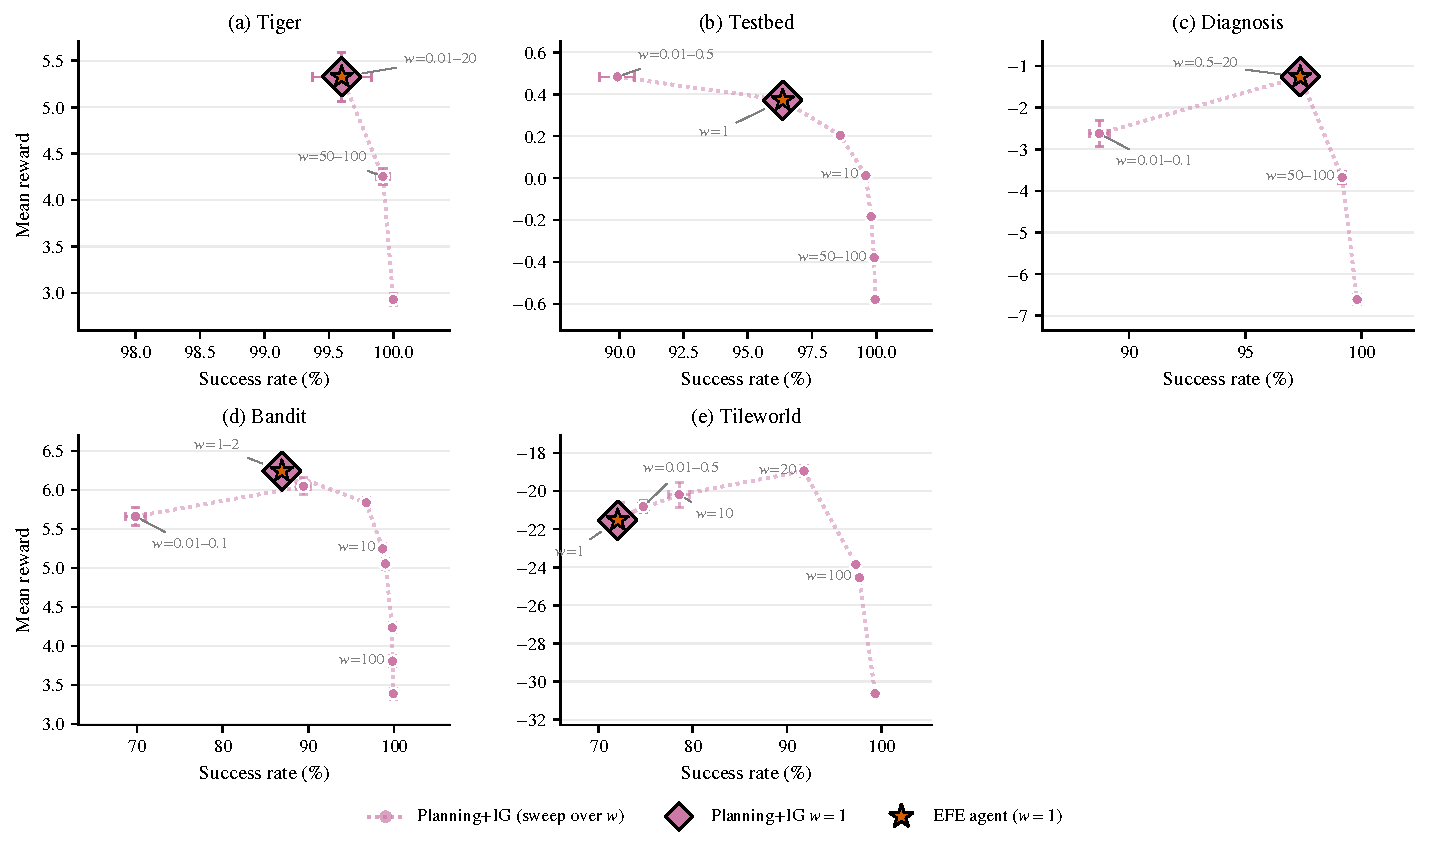
\includegraphics[width=\linewidth]{figures/fig_pareto.pdf}
\caption{Pareto analysis: success rate vs.\ mean reward as $w$ varies from 0.01 to 200. Diamond: Planning+IG at $w{=}1$. Star: EFE agent. By Proposition~\ref{prop:equivalence} with shared deterministic tie-breaking, the markers coincide. Both sit at or near the Pareto knee, where further weight increases buy marginal accuracy at substantial reward cost.}
\label{fig:pareto}
\end{figure}

On every environment in the Pareto sweep, $w{=}1$ sits near the reward-maximizing weight $w^*_{\text{ret}}$, while the success-maximizing weight $w^*_{\text{succ}}$ lies at $20$--$200$ (RockSample and Structural Inspection are not part of the sweep and are discussed separately in Section~\ref{sec:rocksample}). We emphasize that $w{=}1$ is near-optimal for reward, not for success rate: agents requiring near-certain accuracy (e.g., safety-critical applications) would benefit from higher weights at the cost of reduced reward. The contribution of EFE is deriving a principled weight from the variational bound that is near-optimal for reward maximization, rather than a grid search whose optimum changes by orders of magnitude across tasks.

\subsection{Tileworld: spatial epistemic foraging}
\label{sec:tileworld}

To test whether EFE's advantage extends to larger state spaces, we introduce a spatial generalization: the Tileworld projects the Diagnosis partition structure onto an $N{\times}N$ grid ($|S|{=}N^2$), producing spatially interpretable belief evolution (Figure~\ref{fig:tw_comparison}, with step-by-step belief strips in Appendix~\ref{app:tw_belief}).

\begin{table}[ht]
\centering
\caption{Tileworld $6{\times}6$ (2{,}500 episodes: 500 per seed $\times$ 5 seeds, $H{=}2$). Tuned weight $w^*_{\mathrm{succ}}{=}50$.}
\label{tab:tileworld}
\begin{small}
\begin{tabular}{lccc}
\toprule
Agent & Scans & Success & Reward \\
\midrule
Myopic & $0.00$ & 2.9\% & $-48.25$ \\
Planning ($H{=}2$) & $15.64$ & $\mathbf{73.8\%}$ & $\mathbf{-21.39}$ \\
Planning+IG ($w{=}50$) & $32.25$ & 97.3\% & $-23.85$ \\
\textbf{EFE} ($H{=}2$) & $\mathbf{14.75}$ & $\mathbf{72.0\%}$ & $\mathbf{-21.53}$ \\
\bottomrule
\end{tabular}
\end{small}
\end{table}

EFE and reward-only Planning are statistically tied on both reward ($-21.53$ vs.\ $-21.39$, $p{=}0.85$) and success (72.0\% vs.\ 73.8\%, $p{=}0.17$, both bolded in Table~\ref{tab:tileworld}), but EFE reaches that outcome with significantly fewer scans (14.75 vs.\ 15.64, $p<10^{-13}$) -- at this scale, the epistemic bonus shows up in search cost rather than raw reward or success. Planning+IG's 32.25 scans, more than double EFE's, erode reward despite reaching 97.3\% success. The same over-exploration pattern from Diagnosis and Bandit recurs at this larger scale. Figure~\ref{fig:tw_comparison} visualizes the mechanism: EFE concentrates belief efficiently via partition-based narrowing and commits once confident, while Planning lacks scan-selection guidance and Info Gain continues scanning past the point of diminishing returns.

\begin{figure}[t]
\centering
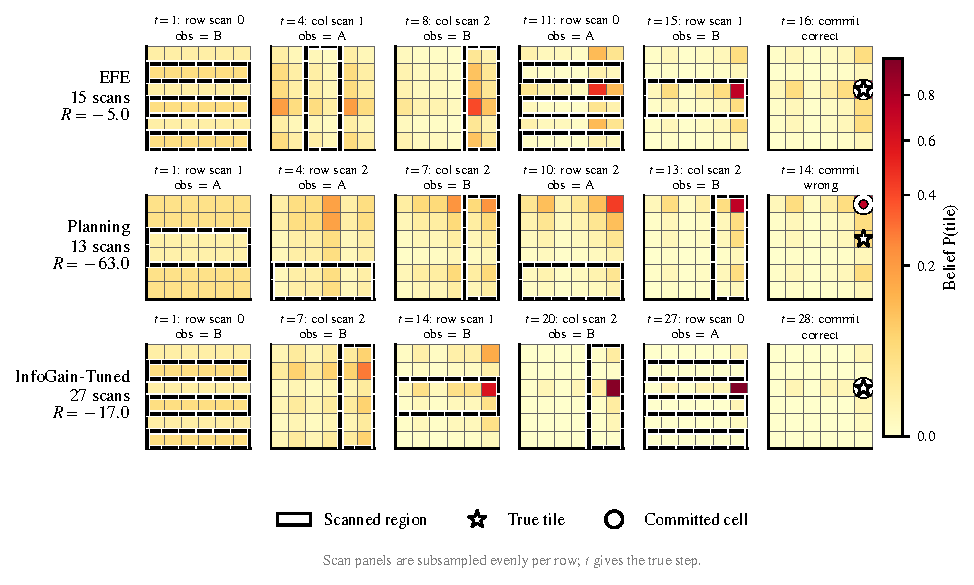
\includegraphics[width=\linewidth]{figures/fig_tileworld_comparison.pdf}
\caption{Agent comparison on the same $6{\times}6$ Tileworld episode. EFE (top) commits correctly with efficient scanning. Planning (middle) explores with less direction before committing. Info Gain (bottom) over-scans well past the point of diminishing returns. Red circle: committed cell. Green star: target.}
\label{fig:tw_comparison}
\end{figure}

\paragraph{Spatial scaling.} We scale the grid from $4{\times}4$ to $8{\times}8$ with all agents (Figure~\ref{fig:tw_scaling}). At $8{\times}8$ ($|S|{=}64$), reward-only Planning collapses to $1.4\%$ success while EFE maintains $69.4\%$. Planning+IG at $w{=}100$ achieves $97.8\%$ success but at substantial reward cost due to extensive scanning. This reveals a nuanced picture: at $4{\times}4$ and $6{\times}6$, EFE's reward and success are within sampling error of reward-only Planning's (within 1 SE at both scales, with Planning nominally slightly ahead on both; no formal test was run for this specific sweep), and EFE's advantage opens up only at $8{\times}8$, exactly where Planning's success collapses. Tuned Planning+IG ($w{=}100$) achieves higher success rates at larger grids by exploring more, at a reward cost due to extensive scanning. Safety-critical applications at large scale would therefore benefit from higher weights.

\begin{figure}[t]
\centering
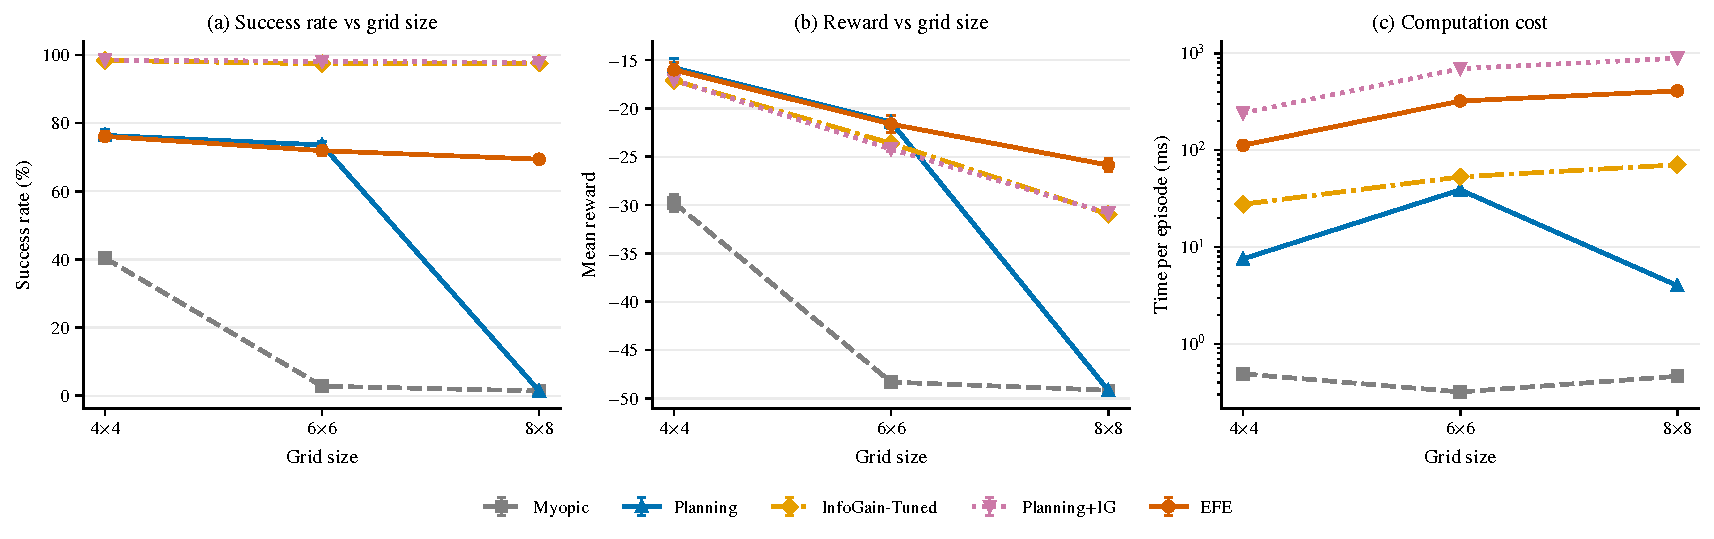
\includegraphics[width=\linewidth]{figures/fig_tileworld_scaling.pdf}
\caption{Tileworld scaling ($H{=}2$, 200 episodes per seed $\times$ 5 seeds) across all agents. Planning collapses at $8{\times}8$ ($|S|{=}64$), while EFE maintains $69.4\%$. Tuned Planning+IG ($w{=}100$) achieves $97.8\%$ but at higher reward cost.}
\label{fig:tw_scaling}
\end{figure}

\paragraph{Observation structure sensitivity.} A natural concern is whether EFE's advantage on Tileworld depends on the highly structured bit-level partition of scan actions. We test this by replacing the deterministic row/column splits with two alternative observation structures: random partitions (each scan randomly assigns cells to two groups, breaking orthogonality) and overlapping partitions (scans use random linear combinations of coordinates, producing correlated and partially redundant observations). On $6{\times}6$ Tileworld ($H{=}2$, 200 episodes $\times$ 5 seeds), EFE and Planning reward $\pm$ episode-level SE are: bitwise $-21.09 \pm 0.86$ (72.8\% success) vs.\ $-21.72 \pm 0.84$ (73.7\%); random $-30.18 \pm 0.94$ (54.9\%) vs.\ $-29.20 \pm 0.94$ (56.6\%); overlapping $-47.87 \pm 0.51$ (7.9\%) vs.\ $-46.12 \pm 0.60$ (11.0\%). EFE's reward advantage over Planning holds only under the structured bitwise partition, and only within roughly one SE there ($-21.09$ vs.\ $-21.72$); it does not show a success advantage over Planning under any partition mode we test here (Planning is nominally ahead on success at bitwise, random, and overlapping alike), and under the random and overlapping partitions EFE is also nominally behind Planning on reward. We read this as an honest boundary of the structured-observation result rather than evidence for a general Planning-vs-EFE ranking under unstructured partitions: with scans that are noisier and less complementary, the epistemic bonus has less useful information to chase, so it stops buying an advantage over reward-only search. As expected, both random and overlapping modes reduce absolute performance for every agent because scans provide less complementary information, but we no longer claim the bitwise-partition ranking is preserved under these alternative observation structures, and we do not claim this experiment establishes EFE's advantage is model-independent.

\subsection{Interleaved observe-act: RockSample}
\label{sec:rocksample}

To exercise Proposition~\ref{prop:factored}'s scope --- its coverage of check and navigation actions --- beyond observe-then-commit settings, we evaluate on RockSample \citep{smith2004}, a standard POMDP benchmark with interleaved observe-act dynamics. An agent navigates an $N{\times}N$ grid containing $K$ rocks at known positions, each with hidden binary quality. Actions include move (N/S/E/W, cost $-0.5$), check rock $k$ (noisy observation, accuracy decays with distance), sample (collect rock at current position: good $+10$, bad $-10$), and exit ($+10$). All agents use depth-limited belief-space tree search over factored beliefs (independent per-rock), differing only in the information gain weight $w$.

% Auto-generated by experiments/build_rocksample_tables.py -- do not edit by hand.
\begin{table}[ht]
\centering
\caption{RockSample results. RS[5,3] and
 RS[7,4]: 500 episodes $\times$ 10 seeds (5{,}000 episodes). RS[7,8]
 and RS[11,11]: 100 episodes $\times$ 5 seeds (500 episodes, reduced
 protocol). Greedy samples without checking. POMCP is the genuine
 search-tree solver at its tuned, frozen configuration (2{,}048
 simulations, Appendix~\ref{app:rocksample}). Rollout only runs
 POMCP's approach-then-check rollout policy standalone, with no
 search tree. Bold marks the best mean reward per instance plus any
 agent not significantly different from it by a seed-level Welch
 $t$-test with Holm--Bonferroni correction, corrected within metric
 (complete pairwise statistics in the committed
 \texttt{results\_rocksample\_*\_stats.csv} files). Reward reported as mean $\pm$
 seed-level SE (SE of the per-seed means, RS[5,3]/RS[7,4]: 10 seeds;
 RS[7,8]/RS[11,11]: 5 seeds).
 Steps and Checks omitted here (per-instance step and check counts,
 and a Flat-MC(1000) reference on every instance, are in
 Appendix~\ref{app:rocksample}).}
\label{tab:rocksample}
\begin{small}
\begin{tabular}{llccc}
\toprule
Instance & Agent & Good & Bad & Reward \\
\midrule
\multirow{6}{*}{RS[5,3]}
 & Greedy & $1.49$ & $1.51$ & $+3.71 \pm 0.26$ \\
 & Planning ($w{=}0$, d=3) & $0.99$ & $0.04$ & $+14.28 \pm 0.13$ \\
 & Plan+IG ($w{=}5$, d=3) & $1.44$ & $0.01$ & $\mathbf{+16.41 \pm 0.13}$ \\
 & EFE ($w{=}1$, d=3) & $1.44$ & $0.03$ & $\mathbf{+16.47 \pm 0.12}$ \\
 & POMCP (2048 sims) & $0.68$ & $0.03$ & $+12.74 \pm 0.11$ \\
 & Rollout only (approach) & $1.41$ & $0.07$ & $\mathbf{+16.67 \pm 0.13}$ \\
\midrule
\multirow{6}{*}{RS[7,4]}
 & Greedy & $1.98$ & $2.02$ & $-1.38 \pm 0.36$ \\
 & Planning ($w{=}0$, d=4) & $0.95$ & $0.05$ & $+13.97 \pm 0.11$ \\
 & Plan+IG ($w{=}5$, d=4) & $1.69$ & $0.01$ & $+14.56 \pm 0.14$ \\
 & EFE ($w{=}1$, d=4) & $1.44$ & $0.01$ & $\mathbf{+15.96 \pm 0.15}$ \\
 & POMCP (2048 sims) & $0.66$ & $0.03$ & $+12.01 \pm 0.06$ \\
 & Rollout only (approach) & $1.88$ & $0.10$ & $\mathbf{+15.85 \pm 0.17}$ \\
\midrule
\multirow{6}{*}{RS[7,8]}
 & Greedy & $4.02$ & $3.98$ & $-5.60 \pm 1.03$ \\
 & Planning ($w{=}0$, d=3) & $0.48$ & $0.03$ & $+12.31 \pm 0.35$ \\
 & Plan+IG ($w{=}5$, d=3) & $3.40$ & $0.01$ & $+23.76 \pm 0.58$ \\
 & EFE ($w{=}1$, d=3) & $2.61$ & $0.06$ & $+21.85 \pm 0.79$ \\
 & POMCP (2048 sims) & $1.71$ & $0.10$ & $+15.07 \pm 0.45$ \\
 & Rollout only (approach) & $3.83$ & $0.19$ & $\mathbf{+28.33 \pm 0.82}$ \\
\midrule
\multirow{6}{*}{RS[11,11]}
 & Greedy & $5.48$ & $5.52$ & $-18.90 \pm 1.04$ \\
 & Planning ($w{=}0$, d=2) & $0.48$ & $0.03$ & $+13.23 \pm 0.18$ \\
 & Plan+IG ($w{=}5$, d=2) & $0.50$ & $0.03$ & $+13.18 \pm 0.15$ \\
 & EFE ($w{=}1$, d=2) & $0.48$ & $0.03$ & $+13.23 \pm 0.18$ \\
 & POMCP (2048 sims) & $0.49$ & $0.03$ & $+12.94 \pm 0.24$ \\
 & Rollout only (approach) & $5.22$ & $0.23$ & $\mathbf{+28.66 \pm 0.83}$ \\
\bottomrule
\end{tabular}
\end{small}
\end{table}


On RS[5,3], EFE and Plan+IG ($w{=}5$) are not significantly different for best reward ($+16.47$ vs.\ $+16.41$, seed-level Welch $p{=}0.74$, both bolded in Table~\ref{tab:rocksample}; this is a failure to reject, not a TOST-backed equivalence claim). On RS[7,4], EFE leads outright ($+15.96$ vs.\ $+14.56$ for Plan+IG, $p<10^{-5}$). On RS[7,8], EFE and Plan+IG ($w{=}5$) are again not significantly different ($+21.85$ vs.\ $+23.76$, $p{=}0.09$ after Holm--Bonferroni correction, both bolded), while both substantially outperform Planning ($+12.31$, $p<10^{-4}$); unlike on RS[5,3] and RS[7,4], more checking does not continue to pay off here, however: Plan+IG ($w{=}10$, Appendix~\ref{app:rocksample}) falls to $+20.55$, significantly below Plan+IG ($w{=}5$) ($p{=}0.003$), so the reward-maximizing weight on this instance is neither $w{=}1$ nor the largest tuned weight but the intermediate $w{=}5$ (not significantly different from $w{=}1$), and pushing the weight higher overshoots into net-negative territory from extra checking cost. The gap vs.\ $w{=}0$ Planning is largest on RS[7,8] among these three instances, though it does not extend to RS[11,11] below, where it vanishes entirely despite that instance having the most rocks to check. On RS[5,3], RS[7,4], and RS[7,8], EFE samples dramatically fewer bad rocks than Greedy (0.01--0.06 vs.\ 1.51--3.98), confirming that the information gain term drives checking behavior.

On RS[11,11] ($|S|{=}2{,}048$), EFE and Planning achieve identical reward ($+13.23$ each), with all information-aware agents vastly outperforming Greedy ($+13.2$ vs.\ $-18.9$), but this does not differentiate EFE from reward-only planning. At the reported depth 2, all informed agents converge to the same conservative ``check nearest rock, sample if good, exit'' strategy, so the weight on information gain never gets to matter. We verified that this is a genuine convergence rather than a depth ceiling: rerunning at depth 3 (\texttt{results\_rocksample\_11x11\_depth3\_check.csv}) costs only seconds and reproduces the same $+13.23$/$+13.17$ pattern within 1 SE, so the earlier claim that depth 3 is computationally intractable at this scale does not hold for the current implementation. The more precise statement is that at $11$ widely spaced rocks under either depth, the greedy nearest-rock heuristic is already close to what shallow tree search recovers, so additional depth or a larger information-gain weight has nothing left to bite on. This mirrors the Tileworld scaling finding (Figure~\ref{fig:tw_scaling}) only in the broad sense that EFE's advantage depends on the state space and rock layout being disambiguating; the specific mechanism here is policy saturation, not a compute ceiling. Detailed results including POMCP baselines on the smaller instances are in Appendix~\ref{app:rocksample}.

\subsection{Structural inspection}
\label{sec:inspection}

To exercise Proposition~\ref{prop:factored}'s scope on a domain-realistic benchmark and demonstrate scalability beyond existing environments, we implement a Structural Inspection POMDP mapping directly to industrial fault detection, medical screening, and non-destructive testing domains. The agent inspects $N$ components arranged spatially, each with a hidden binary state (nominal/faulty). Two non-destructive test types provide accuracy--cost trade-offs: a visual check (accuracy 0.70, cost 0.5) and a detailed test (accuracy 0.90, cost 2.0). The agent navigates between components, selects tests, and declares diagnoses with asymmetric penalties (missed fault $-50$, false alarm $-5$). Tests do not alter component states, so this is a factored observation POMDP and Proposition~\ref{prop:factored} applies.

\begin{table}[ht]
\centering
\caption{Structural Inspection results. $N{=}8$ and $N{=}16$: 2{,}500 episodes each (500 per seed $\times$ 5 seeds). Reward and Accuracy: mean $\pm$ seed-level SE (SE of the 5 per-seed means). Greedy diagnoses without testing. Bold: best accuracy / best reward per instance (not always the same agent). EFE is a competitive untuned trade-off, not uniquely best on all metrics. Accuracy: fraction of components correctly diagnosed.}
\label{tab:inspection}
\begin{small}
\begin{tabular}{llccccc}
\toprule
Instance & Agent & Accuracy & Missed & Tests & Reward \\
\midrule
\multirow{4}{*}{\shortstack[l]{$N{=}8$\\[-1pt]{\scriptsize $|S|{=}256$}}} & Greedy & $70.7 \pm 0.5\%$ & $2.34$ & $0.0$ & $-114.33 \pm 1.96$ \\
& Planning ($w{=}0$) & $73.0 \pm 0.3\%$ & $0.07$ & $12.7$ & $\mathbf{-17.85 \pm 0.23}$ \\
& Planning+IG ($w{=}5$) & $\mathbf{96.3 \pm 0.1\%}$ & $0.10$ & $19.7$ & $-27.98 \pm 0.44$ \\
& EFE ($w{=}1$) & $91.1 \pm 0.2\%$ & $0.09$ & $15.5$ & $-20.95 \pm 0.30$ \\
\midrule
\multirow{4}{*}{\shortstack[l]{$N{=}16$\\[-1pt]{\scriptsize $|S|{=}65{,}536$}}} & Greedy & $70.5 \pm 0.4\%$ & $4.72$ & $0.0$ & $-233.09 \pm 3.13$ \\
& Planning ($w{=}0$) & $78.2 \pm 0.2\%$ & $0.24$ & $22.4$ & $\mathbf{-45.42 \pm 0.23}$ \\
& Planning+IG ($w{=}5$) & $\mathbf{97.3 \pm 0.0\%}$ & $0.14$ & $38.3$ & $-54.74 \pm 0.40$ \\
& EFE ($w{=}1$) & $90.8 \pm 0.1\%$ & $0.24$ & $28.1$ & $-45.80 \pm 0.60$ \\
\bottomrule
\end{tabular}
\end{small}
\end{table}

EFE ($w{=}1$) is a competitive untuned trade-off rather than uniquely best. On $N{=}8$ ($|S|{=}256$), Planning wins reward ($-17.85$), while EFE achieves $91.1\%$ accuracy ($-20.95 \pm 0.30$), gaining $+18.0$pp accuracy over Planning ($73.0\%$, seed-level Welch $p<10^{-10}$) at a moderate reward cost. Planning+IG ($w{=}5$) reaches $96.3\%$ accuracy but at $-27.98$ reward, over-testing relative to reward. On $N{=}16$ ($|S|{=}65{,}536$), Planning wins reward outright ($-45.42$, with EFE a statistically indistinguishable close second at $-45.80$, seed-level $p{=}0.57$), while Planning+IG ($w{=}5$) wins accuracy ($97.3\%$) at substantial reward cost ($-54.74$, the worst of the three informed agents) from extensive over-testing (38.3 tests, roughly $36\%$ more than EFE's 28.1). EFE outperforms Planning by $+12.6$pp accuracy ($90.8\%$ vs.\ $78.2\%$, seed-level $p<10^{-7}$) at a reward cost of only $0.39$ that is itself not significant, a far better accuracy-per-reward trade than Planning+IG's. This is the largest state space in our evaluation and confirms that the factored belief tree search scales to realistic domains. The asymmetric penalty structure ($\alpha = 25$) places this in the regime where Proposition~\ref{prop:nearopt} predicts $w{=}1$ is a reasonable untuned default.

\subsection{Summary}

Taken together, the experiments tell a consistent story. The behavior predicted by Propositions~\ref{prop:equivalence} and~\ref{prop:factored} is what we observe: EFE matches Planning+IG at $w{=}1$ within their stated scope, and that information-unit weight lands at the Pareto knee without per-environment search. Where multiple observation actions matter most, as on Diagnosis and Bandit, untuned EFE Pareto-dominates same-horizon planning. Where tuned bonuses chase success harder, they can beat EFE on accuracy at a reward cost. Across Tileworld, RockSample, and Inspection, EFE remains a competitive untuned trade-off rather than uniquely best on every metric, with the advantage over $w{=}0$ Planning growing as state spaces and observation menus expand, up to $|S|{=}65{,}536$ on Inspection.

\section{Experiments: shadow prices and sensing budgets}
\label{sec:budget_experiments}

Section~\ref{sec:results} evaluated the equivalence and near-optimality claims of Sections~\ref{sec:methodology}--\ref{sec:experiments}. This section evaluates the budgeted reformulation of Section~\ref{sec:budget}: usage-curve collapse across reward scales, closed-form onset recovery, online tracking through a reward rescale, cost-denominated budgets, interleaved (non-observe-then-commit) settings, a near-optimal offline reference, an atlas of implicit budgets, and an explicit test of what the budget does and does not fix. All headline runs use five seeds $\{42,123,456,789,1024\}$ and $100$ episodes per evaluation cell unless noted; code and CSVs accompany the repository.

\subsection{Curve collapse across reward scales}
\label{sec:collapse}

On Diagnosis and Bandit we estimate $U(w;\alpha)$ at reward scales $\alpha \in \{0.1, 1, 10\}$ on $\alpha$-scaled weight grids so that $w/\alpha$ abscissae align. Figure~\ref{fig:collapse} shows the curves collapsing on Diagnosis: every matched $w/\alpha$ point coincides exactly across scales (bit-exact, not merely within $2\cdot\mathrm{SE}$, under the per-episode seeded pipeline), and the crossing bracket of budget $B{=}8$ in $w/\alpha$ units coincides across $\alpha$ ($(0.141, 0.323]$ at every scale). We extend the check to Tiger and Tileworld-$6{\times}6$ to avoid resting the headline claim on two environments (Table~\ref{tab:collapse-breadth}).

\begin{figure}[t]
\centering
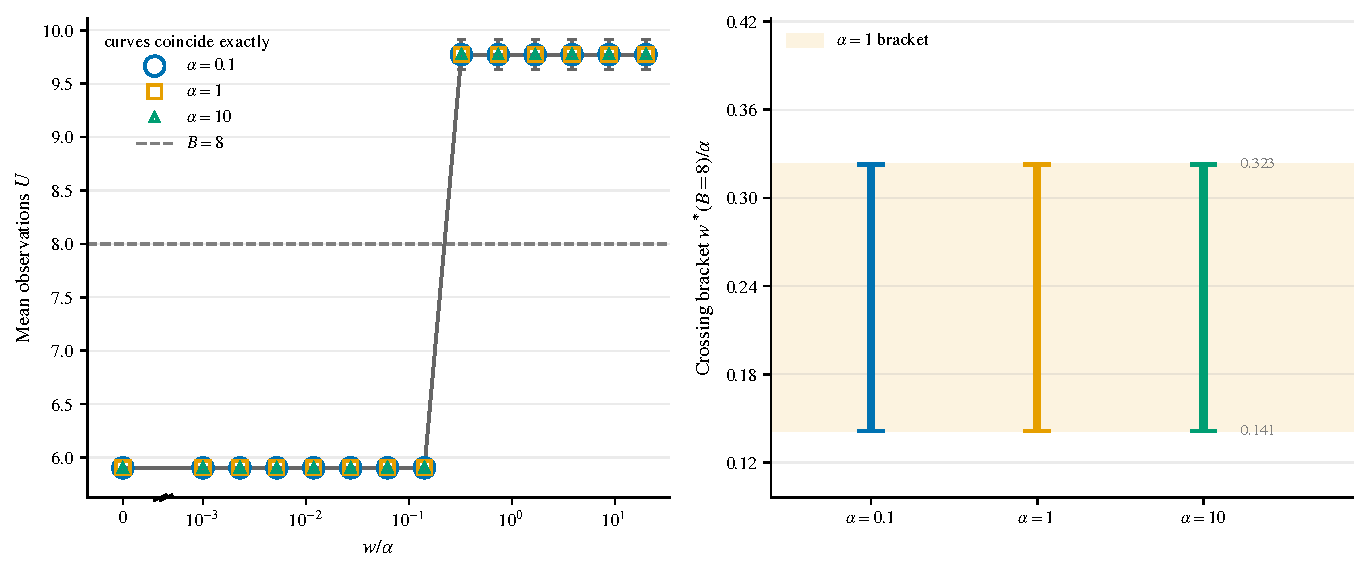
\includegraphics[width=0.85\textwidth]{figures/price_scale_invariance.pdf}
\caption{Curve collapse on Diagnosis. Left: $U$ vs.\ $w/\alpha$ at three reward scales. Right: crossing brackets of $B{=}8$ in $w/\alpha$ units coincide across scales (set-valued shadow price).}
\label{fig:collapse}
\end{figure}

\begin{table}[t]
\centering
\caption{Curve-collapse breadth: fraction of matched $w/\alpha$ points across $\alpha \in \{0.1,1,10\}$ within $2\cdot\mathrm{SE}$, and whether the $B$-crossing bracket coincides across scales (in $w/\alpha$ units).}
\label{tab:collapse-breadth}
\small
\begin{tabular}{lccp{4.3cm}}
\toprule
Environment & Within $2\cdot\mathrm{SE}$ & Max spread & Bracket at $B$ \\
\midrule
Diagnosis ($B{=}8$) & $100\%$ & $0.00$ obs.\ (bit-exact) & $(0.141, 0.323]$ at every $\alpha$ \\
Bandit ($B{=}8$) & $100\%$ & $0.00$ obs.\ (bit-exact) & $(3.84, 8.76]$ at every $\alpha$ \\
Tiger ($B{=}4$) & $100\%$ (trivial) & $0.00$ obs.\ (bit-exact) & unbracketed: $B$ below observed $U$ at every $\alpha$ \\
Tileworld-$6{\times}6$ ($B{=}15$) & $100\%$ & $0.00$ obs.\ (bit-exact) & $(5.80, 20.0]$ at every $\alpha$ \\
\bottomrule
\end{tabular}
\end{table}

Every environment now shows bit-exact collapse: every matched $w/\alpha$ point coincides exactly across the three scales, not merely within Monte Carlo tolerance, and every crossing bracket coincides across scales down to floating-point noise ($\le 10^{-15}$). This is a direct consequence of the per-episode environment seeding fix (Section~\ref{sec:experiments}): under the earlier entropy-seeded environment streams, this same check reported $98\%$ agreement with a nonzero maximum spread, which measured that seeding bug's cross-scale sampling noise as much as genuine Monte Carlo variance; correcting the seeding turns Proposition~\ref{prop:pi1}'s theorem into an equally exact empirical replay, the strongest form the check can take. Diagnosis and Bandit exhibit the exact collapse the proposition guarantees. Tiger passes trivially: instrumental listening already saturates usage ($4.0$--$4.4$ observations) across the entire $w/\alpha \in [0,20]$ range tested, so the budget formulation has no usable dial in this window --- worth stating plainly, since Proposition~\ref{prop:pi1} guarantees collapse of whatever curve there is, not that every environment has an informative curve to collapse. Tileworld-$6{\times}6$'s bracket, which previously showed a knot-sharing discrepancy at the $\alpha{=}10$ scale attributable to budget-at-knot Monte Carlo noise, now coincides exactly at $(5.80, 20.0]$ for every scale, resolving that discrepancy rather than merely narrowing it.

\subsection{Proposition~\ref{prop:nearopt} onset on positive-threshold testbeds}
\label{sec:prop2exp}

Standard Tiger and Testbed parameters yield \emph{negative} $w_{\mathrm{thresh}}$, so any $w \ge 0$ observes and the duality check of Corollary~\ref{cor:pi4} is vacuous there. We therefore construct positive-threshold InfoSeeking environments ($p \in \{0.60, 0.58\}$, $c{=}0.3$, $R_\pm = \pm 1$) with closed forms $w_{\mathrm{thresh}} \approx 3.44$ and $7.55$. A refined weight grid around the threshold shows $U{=}0$ at and below $w_{\mathrm{thresh}}$, with onset in $(w_{\mathrm{thresh}}, 1.03\cdot w_{\mathrm{thresh}}]$ on both environments (upper relative error $3\%$, Figure~\ref{fig:prop2}), matching Corollary~\ref{cor:pi4}. Negative-threshold sanity checks on standard Testbed and Tiger remain consistent ($U(0) > 0$ when $w_{\mathrm{thresh}} < 0$).

\begin{figure}[t]
\centering
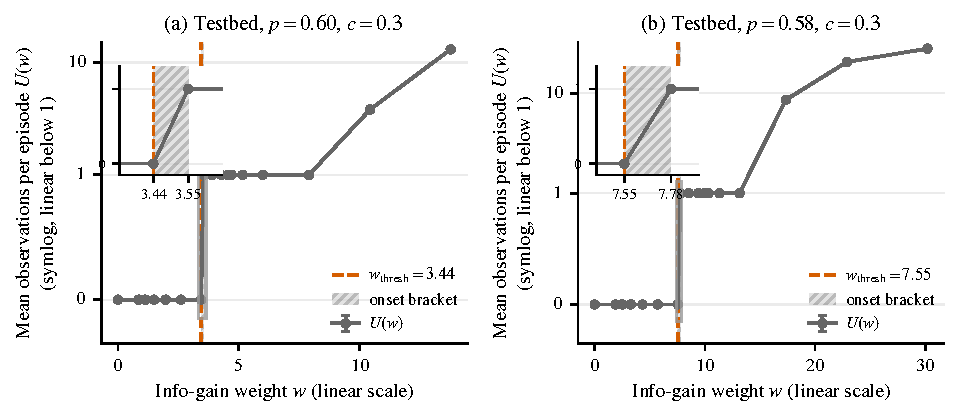
\includegraphics[width=\textwidth]{figures/price_prop2_jumps.pdf}
\caption{Onset of observing on positive-threshold testbeds. Orange: $H{=}1$ closed form (Proposition~\ref{prop:nearopt}). Green band: empirical onset bracket after grid refinement.}
\label{fig:prop2}
\end{figure}

\subsection{Multi-seed online dual control under reward rescale}
\label{sec:dual_multiseed}

On Diagnosis with target $B{=}8$, learning rate $\eta_0{=}0.05$, decay $\delta{=}0.02$, and a $\times 10$ reward-and-cost rescale at episode~$200$ of a $400$-episode run, we sweep $10$ independent controller seeds for decay-only and reset-on-shift variants (window~$20$, $k{=}3$, absolute floor $0.5$), extending the single-trajectory workshop result to a multi-seed comparison with confidence intervals. Re-adaptation is measured as episodes from rescale until rolling-20 usage, computed strictly from post-rescale episodes only, stays within $\pm 1$ of $B$ for $20$ consecutive episodes; an earlier version of this metric let the rolling window straddle the rescale point, which could report a spuriously fast recovery by mixing in the already-converged pre-rescale usage, and we have corrected it (\texttt{experiments/run\_price\_of\_information.py:readaptation\_episodes}). Under the corrected metric: decay-only mean $150.9$ episodes, $95\%$ CI $[142.9, 158.9]$, with $10/10$ seeds recovering inside the $200$ post-rescale episodes; reset-on-shift mean $57.0$, CI $[52.0, 62.0]$, $10/10$ recovered, all but one seed triggering exactly one learning-rate reset (one seed triggers two). The CIs are disjoint, and reset-on-shift re-adapts roughly $2.65\times$ faster than decay alone. Post-rescale steady-state $|U-B|$ is $0.10$ ($[0.056,0.144]$) under reset versus $0.19$ ($[0.061,0.323]$) under decay-only; pre-rescale steady-state error is $0.15$ ($[0.095,0.209]$) for both variants (identical, since decay and reset only diverge after the rescale), close to the tolerance used to declare recovery. Figure~\ref{fig:dualmultiseed} shows the median trajectory with interquartile band for both variants.

\begin{figure}[t]
\centering
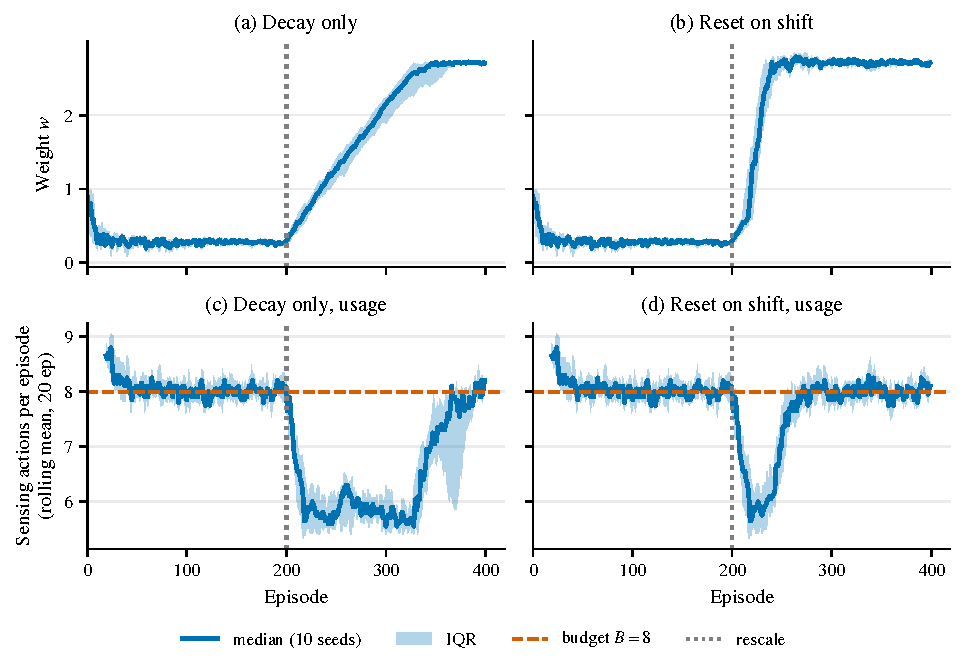
\includegraphics[width=0.85\textwidth]{figures/price_dual_multiseed.pdf}
\caption{Multi-seed ($n{=}10$) dual control of $w$ on Diagnosis through a mid-run $\times 10$ reward rescale (vertical line). Median trajectory with interquartile band; decay-only (left) vs.\ reset-on-shift (right). Reset-on-shift re-adapts in a mean of $57$ episodes vs.\ $151$ for decay alone (post-shift-only rolling window), with disjoint 95\% CIs.}
\label{fig:dualmultiseed}
\end{figure}

The multi-seed result strengthens rather than merely replicates the single-trajectory workshop finding: under the corrected pipeline, both variants now recover on all $10$ seeds tested within the $200$-episode post-rescale window, but decay-only takes roughly $2.65\times$ longer on average and reaches a looser post-rescale steady state, whereas reset-on-shift recovers faster and tighter on every seed. This is the empirical nonstationary re-adaptation behavior anticipated by the constant-step design intuition discussed after Proposition~\ref{prop:pi5}; the proposition's stationary convergence guarantee is not being tested here, since the environment is deliberately shifted mid-run.

\subsection{Cost-denominated budgets}
\label{sec:cost_budget}

The count-usage curves above treat every observation as one unit regardless of price. To demonstrate the units story end to end, we introduce a Diagnosis variant with heterogeneous per-test costs ($[0.5, 2.5]$ across the two test types, same accuracy) and estimate both the count-usage curve $U_{\mathrm{count}}(w)$ and the cost-usage curve $U_{\mathrm{cost}}(w)$ on the same agent family. The mean cost paid per test, $U_{\mathrm{cost}}(w)/U_{\mathrm{count}}(w)$, is not constant: it varies from $1.26$ to $1.41$ across the weight grid (a $12.0\%$ relative spread), rising as high $w$ pushes the agent onto relatively more of the expensive test. This confirms the units story directly: a count budget cannot see that the agent's test mix shifts toward the more expensive test as $w$ rises, while a cost budget prices that shift. At the two comparable operating points we solve for, however, the two denominations happen to land in the same crossing bracket at this grid's resolution: a count budget $B{=}8.86$ brackets $w^*$ in $(10, 31.6]$, and a cost budget $B_{\mathrm{cost}}{=}11.50$ (a comparable operating point in dollars-of-sensing rather than test-count) also brackets $w^*$ in $(10, 31.6]$ (Figure~\ref{fig:costbudget}); the same coincidence holds at the higher pair of budgets we test ($B{=}13.71$ count, $B_{\mathrm{cost}}{=}19.20$ cost, both bracketing $w^*$ in $(31.6, 100]$). We report this plainly rather than as the sharper two-different-brackets demonstration an earlier, unseeded run of this experiment happened to show: with a $12\%$ cost-ratio spread and log-spaced grid knots roughly $2$--$3\times$ apart, the two denominations are not guaranteed to disagree at every tested budget pair, only to disagree in general when the ratio's variation is large enough relative to the grid's resolution.

\begin{figure}[t]
\centering
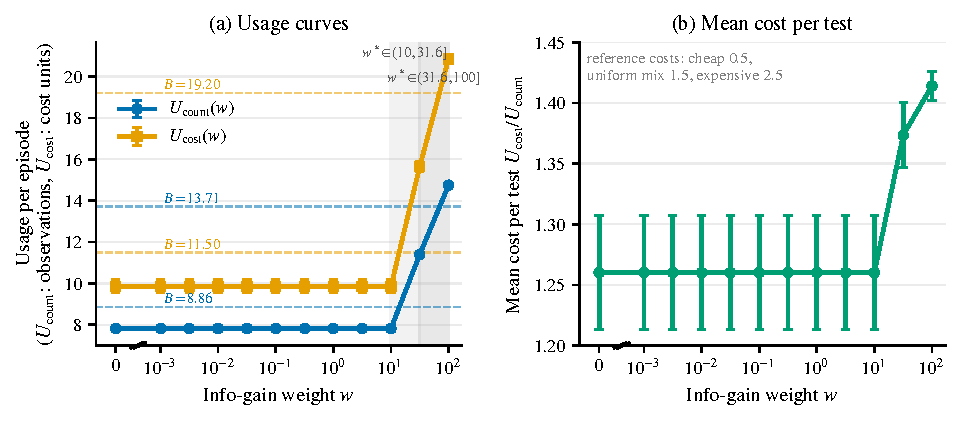
\includegraphics[width=0.85\textwidth]{figures/price_cost_budget.pdf}
\caption{Cost- vs.\ count-denominated usage curves on heterogeneous-cost Diagnosis. The two curves and their crossing brackets disagree because sensing cost per test is not constant across $w$.}
\label{fig:costbudget}
\end{figure}

\subsection{Interleaved settings: RockSample and Structural Inspection}
\label{sec:interleaved_budget}

The observe-then-commit environments above cannot exercise every structural feature of Proposition~\ref{prop:factored}'s factored-observation class, since observation and commitment are temporally separated by construction. We extend usage-curve estimation to the interleaved tree-search agents of Section~\ref{sec:rocksample} and Section~\ref{sec:inspection}, counting check/test actions as sensing usage: RockSample[5,3] (usage range $[3.00, 8.83]$ over a $10$-point weight grid, $5$ seeds $\times$ $50$ episodes), RockSample[7,4] ($[2.00, 14.54]$, $8$-point grid, $30$ episodes), and Inspection-$N{=}16$ ($[22.38, 58.56]$, $10$-point grid, $50$ episodes). Figure~\ref{fig:interleaved} shows all three staircases. $U(w)$ is nondecreasing at \emph{every} sampled grid point on RockSample[7,4] and Inspection-$N{=}16$, a cleaner monotonicity than Tiger, Diagnosis, and Tileworld exhibit (Section~\ref{sec:stairs}); RockSample[5,3] is the exception, dipping from its instrumental floor $U(0){=}3.70$ down to $3.00$ at $w{=}0.316$ before rising, the same kind of non-monotone dip the observe-then-commit environments show, so the interleaved class does not uniformly enjoy the cleaner monotonicity we previously reported for all three instances. At least four budgets are bracketed with SEs per environment. The large instrumental floors ($U(0) = 3.70$ / $2.00$ / $22.38$) confirm that unachievable-low-budget regimes (Definition~\ref{def:pi3}) matter in interleaved settings too: an agent cannot buy less sensing than reward alone already motivates.

\begin{figure}[t]
\centering
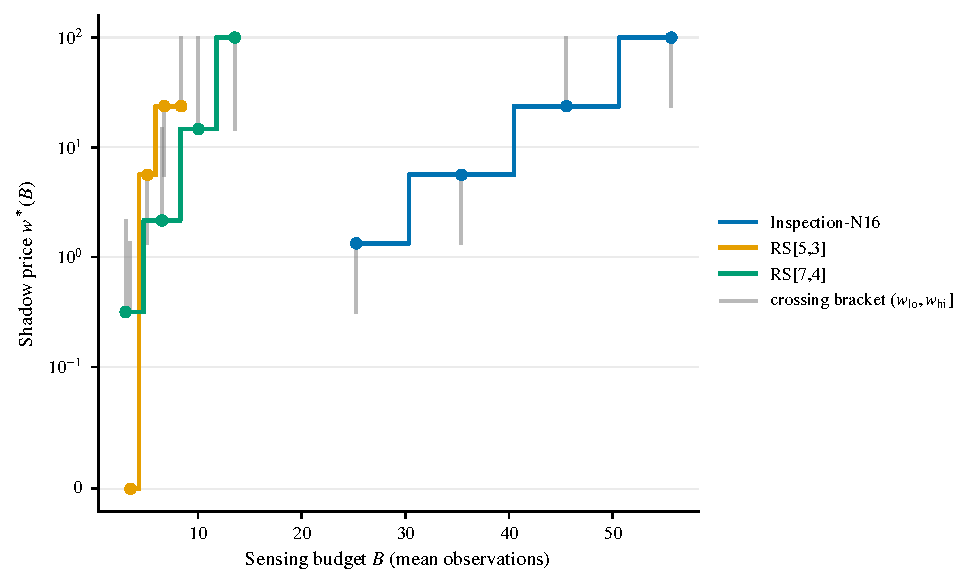
\includegraphics[width=0.85\textwidth]{figures/price_staircase_interleaved.pdf}
\caption{Usage staircases on interleaved (non-observe-then-commit) settings: RockSample[5,3], RockSample[7,4], and Inspection-$N{=}16$. RockSample[7,4] and Inspection-$N{=}16$ are monotone at every sampled grid point; RockSample[5,3] dips once near $w{=}0.316$ before rising.}
\label{fig:interleaved}
\end{figure}

\subsection{Supporting: shadow-price staircases}
\label{sec:stairs}

Figure~\ref{fig:stairs} reports $w^*(B)$ over identifiable budgets inside $[U_{\min}, U_{\max}]$ for Tiger, Diagnosis, Bandit, Tileworld-$6{\times}6$, and Inspection-$N{=}8$. Tiger, Diagnosis, and Inspection are exactly nondecreasing at every sampled grid point; Bandit and Tileworld show local non-monotonicity from discrete policy switches (the count-usage gap identified in Proposition~\ref{prop:pi2}'s scope note), so we report brackets and standard errors rather than singleton prices. Tiger's price is weakly identified, consistent with Table~\ref{tab:collapse-breadth}: instrumental listening already saturates most of the usage range at $w{=}0$.

\begin{figure}[t]
\centering
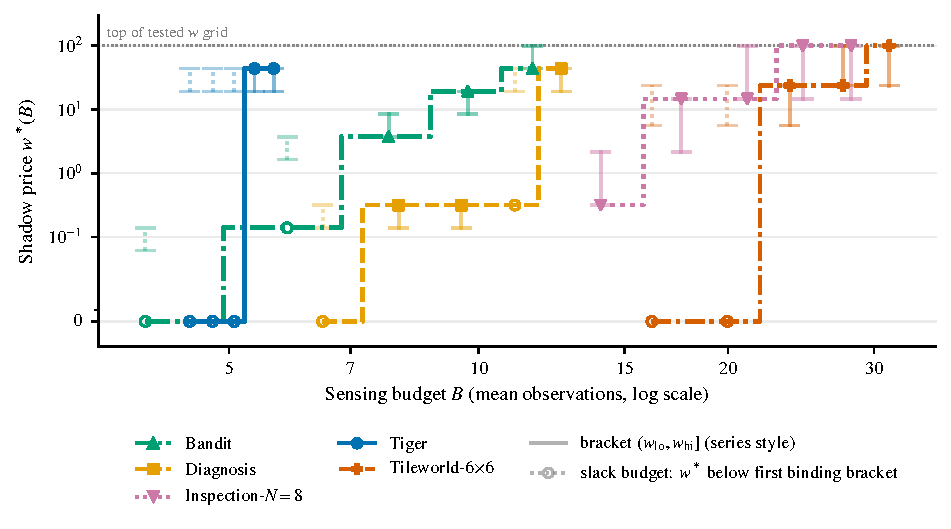
\includegraphics[width=0.85\textwidth]{figures/price_shadow_curves.pdf}
\caption{Operational shadow-price staircases with vertical crossing brackets, observe-then-commit and inspection domains.}
\label{fig:stairs}
\end{figure}

\subsection{A near-optimal offline reference: SARSOP}
\label{sec:sarsop}

The camera-ready replies to the workshop version promised a near-optimal offline baseline; we retire that debt here. We build the original APPL C++ SARSOP toolkit \citep{kurniawati2008} from source (Appendix~\ref{app:sarsop_build}) and export each discrete observe-then-commit benchmark to the Cassandra \texttt{.pomdp} format generically from the same generative model the agents already use, solve to precision $10^{-3}$ (under one second per environment at $\gamma{=}0.999$), and evaluate the resulting alpha-vector policy in-simulator through the identical episode runner used for every other agent, so all agents share mechanics and metrics exactly. Table~\ref{tab:sarsop} reports the full protocol ($5$ seeds $\times$ $500$ episodes).

\begin{table}[t]
\centering
\caption{SARSOP near-optimal reference vs.\ EFE ($w{=}1$) on the three core OTC environments (mean $\pm$ SE reward; mean usage in observation count; $\gamma{=}0.999$).}
\label{tab:sarsop}
\small
\begin{tabular}{lcccc}
\toprule
Environment & SARSOP reward & EFE reward & SARSOP usage & EFE usage \\
\midrule
Tiger & $5.061 \pm 0.158$ & $5.061 \pm 0.158$ & $4.323$ & $4.323$ \\
Diagnosis & $-1.452 \pm 0.336$ & $-1.217 \pm 0.184$ & $9.68$ & $9.73$ \\
Bandit & $6.280 \pm 0.134$ & $6.261 \pm 0.112$ & $5.16$ & $5.09$ \\
\bottomrule
\end{tabular}
\end{table}

On Tiger, SARSOP and EFE select identical actions on every episode: with a single observation action, the near-optimal policy and the EFE policy coincide exactly. On Diagnosis and Bandit, SARSOP and EFE ($w{=}1$) show no statistically significant reward difference at our sample sizes (the Diagnosis means differ by about $0.6$ SE), and their usage differs by less than $0.1$ observations. We formalize this with a predeclared-margin two one-sided tests (TOST) equivalence procedure \citep{schuirmann1987}: the margin is fixed, before inspecting these samples, at the cost of one sensing action in each environment ($\pm 1.0$ reward for Tiger and Diagnosis, $\pm 0.5$ for Bandit, i.e., a reward difference smaller than a single listen/test/inspection is not operationally meaningful here; this is a domain-specific operational margin, not a universal equivalence standard), and the test is an unpaired Welch (unequal-variance) $t$-test on per-seed means ($n{=}5$ seeds, $500$ episodes/seed) rather than pooled episode-level values, so degrees of freedom reflect independent seeds. We do not pair by seed index despite EFE and SARSOP sharing the same nominal seed list: once the two policies' action choices diverge on an episode, they consume the environment's random draws in different orders, so a common seed label does not guarantee correlated trajectories between the two agents, and treating the seeds as paired blocks would understate the true variance. All three environments reject both one-sided nulls at $\alpha{=}0.05$ (Tiger $p{=}0.0010$, Diagnosis $p{=}0.0458$, Bandit $p{=}0.0130$; equivalently, the $90\%$ CI of the mean difference lies entirely inside the margin on all three: Tiger $[-0.41,+0.41]$, Diagnosis $[-0.51,+0.98]$, Bandit $[-0.35,+0.31]$), so we can now state the stronger claim: EFE at the canonical weight is statistically equivalent to the SARSOP reference within the predeclared margin on this suite, not merely consistent with parity (\texttt{results\_tost\_sarsop.csv}). We additionally checked whether the offline usage curve can be inverted to match SARSOP's usage exactly (rather than comparing at $w{=}1$); on Tiger this usage-matching problem is ill-posed because the curve is flat (Table~\ref{tab:collapse-breadth}), forcing a bracket as wide as $w \in (19.3, 43.9]$ to nominally match a target that the curve cannot discriminate. We considered POMCPOW \citep{sunberg2018} as a further baseline and declined it: POMCPOW exists to handle continuous state, action, and observation spaces via progressive widening, and every benchmark here is a small discrete POMDP for which SARSOP already gives a near-optimal reference and discrete POMCP (Appendix~\ref{app:pomcp}) is already in hand; adding POMCPOW would require building continuous-observation benchmark variants that no claim in this paper needs.

\subsection{A near-optimal constrained-POMDP reference}
\label{sec:cpomdp}

Both referee passes on this manuscript converged on the same top-priority addition: a constrained-POMDP (CPOMDP) comparison that goes beyond the additive Planning+IG family, rather than treating its absence as a permanent disclosed limitation. We now provide one for the three environments where SARSOP already serves as our near-optimal reference (Tiger, Diagnosis, Bandit; Section~\ref{sec:sarsop}), by extending the same SARSOP export with a literal per-unit usage penalty in the reward model: each observation action's reward becomes $-(\text{cost}_j + \lambda)$ for $\lambda \ge 0$, so solving the resulting POMDP to SARSOP's precision ($10^{-3}$) gives, for that $\lambda$, a near-optimal solution to $\max_\pi \mathbb{E}_\pi[R] - \lambda\,\mathbb{E}_\pi[U]$ over the \emph{full} space of POMDP policies (not the additive Planning+IG family) -- near-optimal rather than certified-exact because SARSOP is a point-based approximate solver and the reported reward and usage are themselves Monte Carlo estimates from simulated episodes, not closed-form quantities. For a finite discounted constrained MDP, strong Lagrangian duality holds \citep{altman1999}: sweeping $\lambda$ over a log-spaced $12$-point grid ($\lambda \in [0, 100]$, $\gamma{=}0.999$, $5$ seeds $\times$ $300$ episodes per $\lambda$) traces an estimated upper concave envelope of the achievable $(\mathbb{E}[U], \mathbb{E}[R])$ region, sampled at these 12 supported points rather than continuously; a per-episode mixture of two adjacent swept policies approximates any intermediate budget, the same mixture argument used for the Planning+IG shadow price (Definition~\ref{def:pi3}), though the approximation inherits whatever slack the constituent near-optimal solutions carry. $\lambda{=}0$ recovers the ordinary reward-only SARSOP solve of Table~\ref{tab:sarsop} as a sanity check.

\begin{table}[h]
\centering
\caption{Estimated CPOMDP reference gap at the budget $B_{\mathrm{EFE}} = U(\text{EFE}, w{=}1)$, interpolated on the Lagrangian-sweep reference frontier. $R_{\mathrm{ref}}$ is the near-optimal SARSOP-Lagrangian reward at that usage (not a certified bound); the gap is $R_{\mathrm{ref}} - R_{\mathrm{EFE}}$. Planning+IG at the usage-matched weight $w^*$ (not $w{=}1$: $w^*{=}0.00$, $0.45$, and $1.07$ for Tiger, Diagnosis, and Bandit respectively) attained reward statistically indistinguishable from EFE's on all three environments in this run, an empirical finding about this policy family and this suite, not a consequence of Proposition~\ref{prop:equivalence}, which is stated for $w{=}1$ specifically. A single gap column covers both.}
\label{tab:cpomdp}
\small
\begin{tabular}{lccccc}
\toprule
Environment & $B_{\mathrm{EFE}}$ & $R_{\mathrm{ref}}$ & $R_{\mathrm{EFE}}$ & Gap & Gap \% \\
\midrule
Tiger & $4.32$ & $5.016$ & $5.016$ & $0.000$ & $0.00\%$ \\
Diagnosis & $9.82$ & $-1.297$ & $-1.224$ & $-0.073$ & $-5.65\%$ \\
Bandit & $5.10$ & $6.313$ & $6.320$ & $-0.007$ & $-0.11\%$ \\
\bottomrule
\end{tabular}
\end{table}

The estimated gap is zero on Tiger and within one grid step of zero on Bandit ($-0.11\%$). Diagnosis shows a small negative gap ($-5.65\%$, i.e., the reference value is slightly \emph{below} $R_{\mathrm{EFE}}$): since a true optimum cannot lie below EFE's measured reward, a negative estimated gap indicates reference-frontier noise or resolution limits rather than a real violation. We attribute it to finite-sample noise at the usage ceiling combined with interpolation past the sampled grid: EFE's own measured usage ($9.824$) marginally exceeds the highest usage realized anywhere on the $12$-point $\lambda$ grid ($9.817$, at $\lambda{=}0.107$), so the reported $R_{\mathrm{ref}}$ is the clamped boundary value rather than an interpolation between two bracketing points, and both quantities are themselves $1{,}500$-episode Monte Carlo estimates with standard errors of comparable magnitude to the gap ($\pm 0.13$--$0.31$). A finer $\lambda$ grid near $0$ and more episodes per point would sharpen this estimate; we report the current resolution rather than tuning the grid to close the gap. Read together with Table~\ref{tab:sarsop}'s TOST result, the finding is that the calibrated Planning+IG family is not just close to the single reward-maximizing operating point, but empirically close to this near-optimal reference across the usage range swept, on this three-environment suite (\texttt{results\_cpomdp\_baseline.csv}, \texttt{results\_cpomdp\_frontier.csv}; \texttt{experiments/run\_cpomdp\_baseline.py}).

This provides a near-optimal constrained-POMDP reference for the discrete observe-then-commit suite -- an estimated rather than certified optimality gap, since it rests on an approximate solver evaluated by simulation -- but the scope is deliberately narrow: it does not extend to RockSample or Structural Inspection's larger factored state spaces, where SARSOP itself is no longer a practical solver at the sizes we study (Section~\ref{sec:rocksample}), so even an approximate optimality-gap estimate there remains future work.

\subsection{Distractor robustness: reward-irrelevant sensing}
\label{sec:distractor}

A recurring question about information-gain objectives is how they behave when uncertainty exists over state components that do not affect reward. We construct \texttt{DistractorDiagnosisEnv}, an $8$-joint-state Diagnosis variant ($4$ conditions $\times$ a binary nuisance bit; commit rewards depend only on the $4$-way condition) with one additional test that is informative only about the nuisance bit. Every observation model in the environment factors through exactly one of the two independent components, so the distractor test is provably --- and unit-tested --- exactly zero-information about the condition marginal.

Sweeping Planning+IG over a log weight grid ($5$ seeds $\times$ $100$ episodes), the distractor fraction of total sensing usage is exactly $0$ for $w \le 3.16$, rises to $0.233 \pm 0.005$ at $w{=}10$, and saturates in the $0.330$--$0.332 \pm 0.005$ range for $w \ge 31.6$ (Figure~\ref{fig:distractor}). Ordinary information gain does not distinguish reward-relevant from reward-irrelevant uncertainty, so once the weight is large enough to make the distractor's nonzero (but task-useless) information gain worth its cost, Planning+IG spends budget on it; the sensing budget of Section~\ref{sec:budget} caps how much total sensing is bought but does not by itself redirect that spending toward reward-relevant tests. EFE at the canonical $w{=}1$ happens to stay at zero distractor fraction on this instance, but only because the onset weight ($\approx 10$) exceeds $1$ here, not because EFE is structurally immune to the effect; an instance with a lower onset would show EFE chasing the distractor too.

\begin{figure}[t]
\centering
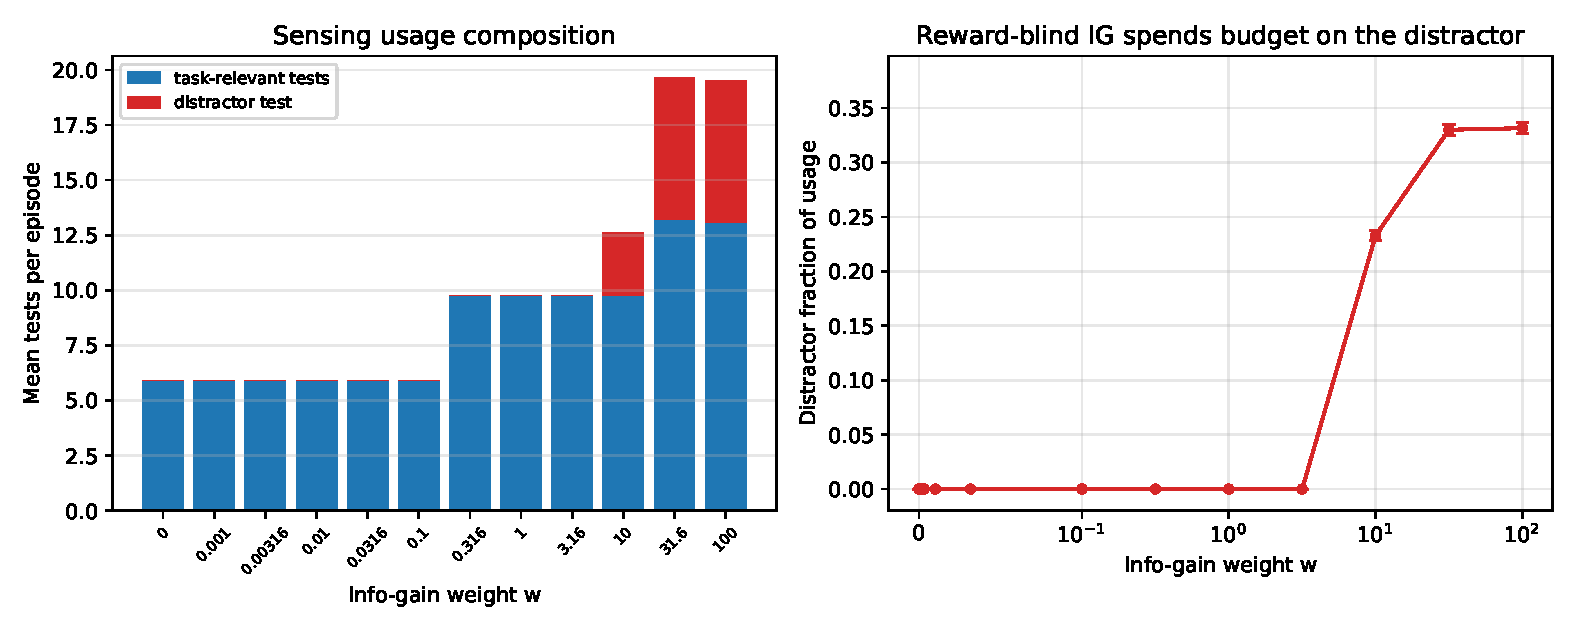
\includegraphics[width=0.85\textwidth]{figures/distractor_composition.pdf}
\caption{Usage composition on \texttt{DistractorDiagnosisEnv} as a function of $w$: task-relevant test usage, distractor test usage, and their sum. Distractor spend is zero below the onset weight and saturates at roughly a third of total usage.}
\label{fig:distractor}
\end{figure}

We also checked whether information-directed sampling (IDS) \citep{russo2014}, which is explicitly reward-aware through its information-ratio numerator, is immune. It is not, for an implementation reason worth reporting exactly: IDS's \texttt{info\_astar} term (information about the optimal commit) is correctly zero for the distractor action, but the implementation falls back to a raw state-entropy term (\texttt{info\_state}) whenever \texttt{info\_astar} is at or near zero, and that fallback lets the distractor's genuine nuisance-bit informativeness through. Instrumented directly, IDS's distractor fraction is $0.305 \pm 0.005$, comparable to Planning+IG at large $w$. This is not evidence that reward-aware information measures are useless against distractors in general; it is evidence that a specific, common implementation pattern (falling back to unconditional entropy reduction when the reward-conditional information measure vanishes) reintroduces exactly the reward-blindness the reward-aware measure was meant to avoid. We report this as an honest limitation rather than eliding it: neither ordinary information gain nor the in-repo IDS adaptation is a clean immune baseline against reward-irrelevant sensing on this benchmark, and a genuinely reward-conditional information measure without a raw-entropy fallback is left to future work.

\subsection{The $w^*$ atlas}
\label{sec:w_atlas}

Table~\ref{tab:w-atlas} (Appendix~\ref{app:w_atlas}) collects the implicit EFE budget $B_{\mathrm{EFE}} = U(w{=}1)$ and two canonical-budget crossing brackets for every benchmark instance in this paper, aggregating the usage curves estimated across Sections~\ref{sec:results} and~\ref{sec:budget_experiments}. This is an atlas of measured operating points, not a predictive meta-model relating $B_{\mathrm{EFE}}$ to environment parameters (reward scale, state count, horizon); no such closed form is claimed, and the atlas should not be read as one.

\section{Discussion}
\label{sec:discussion}

\paragraph{When does EFE-as-$\rho$ help?}
EFE's advantage requires two conditions: (1)~multiple observation actions with differential informativeness, and (2)~sufficient planning horizon for recursive EFE to propagate epistemic value. When condition (1) fails, as on Tiger with its single listen action, reward-only planning matches EFE. The Tileworld adds a third axis: as the state space grows, the reward signal becomes too diffuse to guide scan selection, and EFE's advantage increases (Figure~\ref{fig:tw_scaling}). Within-episode dynamics (Appendix~\ref{app:foraging}) show the mechanism: EFE concentrates belief via partition-based narrowing and commits once the value of committing exceeds the value of observing, a crossover that emerges automatically from $w{=}1$ without tuning (Figure~\ref{fig:traj}, Appendix~\ref{app:efe_trajectory}).

\paragraph{The information-unit weight and why it works.}
EFE does not eliminate the exploration--exploitation weight. It supplies a derived relative coefficient in information units under a fixed reward convention. The Pareto analysis (Figure~\ref{fig:pareto}) shows this weight sits near the reward-maximizing $w^*_{\text{ret}}$ on every environment in the sweep, while the success-maximizing $w^*_{\text{succ}}$ (used for Planning+IG in the main tables) lies at $20$--$200$. The gap between $w^*_{\text{ret}}$ and $w^*_{\text{succ}}$ has practical implications: $w{=}1$ targets expected reward, not success probability. In safety-critical settings where near-certain accuracy is required, a higher weight may be appropriate, though such weights must still be tuned per-environment. EFE provides a principled starting point rather than a scale-free automatic calibration. Increasing $w$ beyond 1 buys marginal accuracy at substantial reward cost. Moreover, adding planning depth to a weighted IG bonus amplifies the weight's effect ($w{=}100$ on Bandit: Planning+IG takes 12.41 inspections vs.\ myopic Info Gain's 10.99), making the tuning problem harder with depth. Identifying pragmatic value with task reward chooses $P(o|C) \propto \exp(\beta R)$ with $\beta{=}1$ per reward unit, so keeping $w$ fixed while rescaling rewards by $k$ rescales the effective weight by $1/k$. The claim is exact under log scoring rules \citep{bernardo1979}. Our implementation uses bits ($\mathrm{base}{=}2$). Nat/bit conversion multiplies $w$ by $\ln 2 \approx 0.69$, within the broad Pareto knee where $w \in [0.5, 2.0]$ yields near-identical reward.

The information-unit weight's advantage requires $\gamma \geq 0.99$ on multi-observation environments. Our discount-sensitivity analysis (Appendix~\ref{app:discount}, 5 seeds) reveals a sharp transition: on Diagnosis ($N{=}4$), EFE's success advantage over Planning is $+8.6$pp at $\gamma{=}1.0$ and $+7.9$pp at $\gamma{=}0.99$ (both seed-level Welch $p<10^{-4}$), but is not statistically significant at $\gamma{=}0.95$ or $\gamma{=}0.90$ (diff $\approx 0.04$pp, $p{=}0.96$ at both). The mechanism is that discounting truncates the effective planning horizon below the number of observations needed for confident diagnosis, erasing EFE's advantage. On Tiger (single observation), EFE and Planning differ significantly only at the heaviest discounting tested ($\gamma{=}0.90$, $+2.7$pp, $p<10^{-3}$) and are numerically identical at $\gamma \geq 0.95$. This is a meaningful practical limitation: applications with high time pressure or non-stationary environments that mandate heavy discounting will not benefit from EFE's epistemic drive.

\paragraph{Zero-shot weight transfer.}
The tuning problem is not merely inconvenient. Transfer depends on the tuning criterion. Table~\ref{tab:transfer} evaluates $w{=}1$, reward-tuned weights $w^*_{\mathrm{ret}}$, and success-tuned weights $w^*_{\mathrm{succ}}$ across environments. Success-tuned transfer harms reward: $w^*_{\mathrm{succ}}{=}100$ from Diagnosis yields $+4.25$ on Tiger and $-0.38$ on Testbed versus $w{=}1$ at $+5.33$ and $+0.37$. Reward-tuned moderate weights ($w\in\{0.5,1\}$) transfer much better within the shared reward scale, and $w{=}1$ is tied for best on Tiger and Diagnosis (alongside $w{=}0.5$ and, on this instance, even the success-tuned $w{=}20$, since Tiger's and Diagnosis's reward landscape is flat enough at these weights that several ties collapse together) and remains best outright on Bandit without search. The honest conclusion is that moderate untuned weights are robust under a shared reward convention, while success-tuned weights overfit once pushed to the larger end of the tested grid ($w \geq 50$). In that moderate band, $w{=}1$ is the variational default, not a scale-free optimum.

\begin{table}[ht]
\centering
\caption{Zero-shot weight transfer (500 episodes $\times$ 5 seeds). Rows include $w{=}1$, reward-tuned weights ($w^*_{\mathrm{ret}}$), and success-tuned weights ($w^*_{\mathrm{succ}}$). Success-tuned transfer harms reward. Moderate reward-tuned weights transfer better within the shared reward scale. Bold: best reward per column (Tiger and Diagnosis show a three-way tie among $w \in \{0.5, 1, 20\}$ under the fixed pipeline).}
\label{tab:transfer}
\begin{small}
\begin{tabular}{lcccc}
\toprule
Weight & Tiger & Diagnosis & Bandit & Testbed \\
\midrule
$w{=}0.5$ ($w^*_{\mathrm{ret}}$ Diag./Testbed) & $\mathbf{+5.33}$ & $\mathbf{-1.26}$ & $+6.05$ & $\mathbf{+0.48}$ \\
$w{=}1$ (EFE / $w^*_{\mathrm{ret}}$ Tiger/Bandit) & $\mathbf{+5.33}$ & $\mathbf{-1.26}$ & $\mathbf{+6.24}$ & $+0.37$ \\
$w{=}20$ ($w^*_{\mathrm{succ}}$ Tiger) & $\mathbf{+5.33}$ & $\mathbf{-1.26}$ & $+5.05$ & $-0.18$ \\
$w{=}50$ ($w^*_{\mathrm{succ}}$ Testbed) & $+4.25$ & $-3.68$ & $+4.23$ & $-0.38$ \\
$w{=}100$ ($w^*_{\mathrm{succ}}$ Diag./Bandit) & $+4.25$ & $-3.68$ & $+3.81$ & $-0.38$ \\
\bottomrule
\end{tabular}
\end{small}
\end{table}

\paragraph{When is $w{=}1$ near-optimal?}
Proposition~\ref{prop:nearopt} formalizes lower and upper thresholds for the two-state case: $w^*_{\mathrm{lo}}$ depends on reward asymmetry $\alpha = |R^-|/R^+$, informativeness $\eta = I_{\max}/c$, and accuracy $p$, while $w^*_{\mathrm{hi}}$ bounds over-observation at the post-first-observation belief. Table~\ref{tab:alpha_eta} is consistent with this prediction on the genuinely two-state rows and, more heuristically, on the two-state-reduced rows (Bandit omitted as multi-arm). High-asymmetry environments ($\alpha \geq 5$: Tiger, Diagnosis, Tileworld) have $w^*_{\mathrm{lo}} \ll 0$ and $w^*_{\mathrm{hi}} \approx 7$--$8$, so $w{=}1$ is interior. Testbed places $w{=}1$ near the upper bound, consistent with over-exploration.

To assess whether the $H{=}1$ analysis extends to multi-step planning, we conducted a Monte Carlo study over 100 randomly generated two-state environments (sampling $\alpha \in [1, 50]$, $p \in [0.55, 0.95]$, cost $\in [0.1, 5]$). For each environment and $H \in \{1, 2, 3\}$, we compute the reward-optimal $w^*$ by grid search and classify $w{=}1$ as near-optimal when the reward gap from $w^*$ is within $\max(5\%, 0.5)$ of the best reward (Figure~\ref{fig:nearopt_horizon}). The near-optimality rate increases from 30\% at $H{=}1$ to 58\% at $H{=}2$ and 79\% at $H{=}3$, confirming that multi-step planning amplifies the value of observation and expands the region where $w{=}1$ is near-optimal. High-asymmetry environments ($\alpha \geq 10$) follow the same trend: 26\% $\to$ 53\% $\to$ 79\%. This is qualitatively consistent with the Bandit result: Bandit's reward asymmetry is low relative to the high-asymmetry environments above (correct-arm reward $+10$ vs.\ small-reward-arm $+1$, not the two-state $\alpha{=}|R^-|/R^+$ ratio this section's formula assumes, so we do not report a numeric $\alpha$ for it), so the $H{=}1$ analysis predicts only marginal sufficiency, yet multi-step EFE at $H{=}2$ achieves $86.9\%$ success (Table~\ref{tab:main}).

Many real-world decision problems have $\alpha \gg 1$: in medical diagnosis, fault detection, and security screening, a missed condition costs far more than another test. This is the regime where the interval analysis is most favorable to $w{=}1$, and the multi-step study shows the near-optimality basin widening with planning depth ($79\%$ of $\alpha \ge 10$ environments pass at $H{=}3$, up from $26\%$ at $H{=}1$). The practical consequence is calibrated accordingly: in these domains the information-unit weight is a strong untuned starting default under the shared reward convention, not a guarantee of near-optimality, and the budgeted machinery of Section~\ref{sec:budget} is the recourse when the default's induced sensing does not match what the application can afford.

\paragraph{Robustness to model misspecification.}
Our main results assume exact knowledge of the generative model. Appendix~\ref{app:misspec} investigates robustness when the agent's believed observation accuracy differs from the true value by up to $\pm 0.15$. On Tiger, success rates remain above 96.9\% across all mismatch levels, and EFE and Planning respond identically to every tested mismatch (Table~\ref{tab:misspec-tiger}), so there is no measurable EFE-specific buffering effect on this environment. On Diagnosis, degradation is larger but graceful, and both agents' behavior steps between two levels rather than degrading smoothly with the mismatch magnitude. Overestimating sensor accuracy (positive mismatch) is more harmful than underestimating it, because the agent commits prematurely on insufficient evidence.

\paragraph{Approximate planning with MCTS-EFE.}
At each depth the tree branches over $K$ observation actions and then, per action, over its $|\mathcal{O}|$ observation outcomes, so the exact tree search cost is $\mathcal{O}((K \cdot |\mathcal{O}|)^H)$, limiting practical horizons to $H{=}2$--$3$ with $K \geq 3$. To push beyond this, we implement MCTS with EFE as a leaf heuristic: the tree policy uses UCB1 with observation-outcome enumeration, and leaf nodes are evaluated via greedy EFE rollouts. On Tiger at $H{=}10$, MCTS-EFE with 500 simulations achieves 97.7\% success ($\approx$5.9s per 200 episodes), compared to 88.8\% for POMCP at the same simulation count ($\approx$4.1s; the comparison is simulation-matched, not compute-matched --- MCTS-EFE's leaf evaluations are more expensive per simulation). This shows that EFE's closed-form information valuation provides a substantially stronger leaf heuristic than semi-informed rollouts in this configuration. The comparison avoids a pure-random-rollout strawman: our implementation already uses belief-optimal commits (not purely random rollouts): observations are sampled uniformly, but the rollout terminates with the commit action maximizing expected reward under the Bayesian-updated belief (Appendix~\ref{app:pomcp}). The remaining performance gap therefore reflects the value of directed observation selection: EFE chooses which test to run based on information gain, while POMCP samples tests uniformly. The claim is not that EFE-based planning exceeds state-of-the-art POMDP solvers, but that the EFE leaf heuristic provides a principled, zero-tuning alternative to heuristic rollout design. POMCP with fully informed rollouts (e.g., using domain knowledge or a learned value function for observation selection) would narrow the gap further.

The approach also scales to multiple observation actions. For single-observation environments, the observation-outcome enumeration (2 outcomes per action) keeps expansion costs low. On Diagnosis ($N{=}4$, $K{=}2$ tests), MCTS-EFE at $H{=}5$ achieves $94.2\%$ success compared to POMCP's $68.7\%$ at the same simulation count (200 simulations), demonstrating that EFE scales to multi-observation environments. To validate on a larger multi-observation environment, we evaluate on Tileworld $6{\times}6$ ($|S|{=}36$, $K{=}6$ scans). MCTS-EFE saturates at $95.4\%$ success across both simulation budgets tested (200 and 500), well above Exact-EFE's $71.9\%$, but at a reward cost ($-25.02$ vs.\ Exact-EFE's $-21.62$) from scanning substantially more (32.3 vs.\ 14.8 observations on average): MCTS's sampled rollouts do not value information as precisely as the exact recursion, so it trades reward for a large success-rate gain by scanning more thoroughly, the opposite trade-off from the Tiger and Diagnosis comparisons above, where MCTS-EFE tracked Exact-EFE closely on both metrics. POMCP collapses on this larger observation menu regardless of simulation budget ($10.7\%$ at 200 simulations, $5.6\%$ at 500), so MCTS-EFE's $85$--$90$pp success-rate gap over POMCP indicates that directed observation selection remains essential at this scale even though the specific reward/success trade-off MCTS-EFE strikes here differs from the smaller environments: semi-informed rollouts still cannot identify which of the 6 scans to perform. For larger observation spaces, more efficient tree policies, such as progressive widening or double progressive widening \citep{benchetrit2025}, would further improve scalability. We leave this to future work.

\paragraph{When to use EFE-as-$\rho$: summary.}
Our analysis identifies the following conditions favoring EFE over tuned alternatives:
\begin{itemize}[leftmargin=1.5em,itemsep=1pt,topsep=2pt]
\item Reward asymmetry $\alpha \geq 5$: the penalty for a wrong commit far exceeds the observation cost, placing $w{=}1$ well inside the $H{=}1$ near-optimality interval on our suite (Proposition~\ref{prop:nearopt}); the random-environment study tempers this into a favorable-regime heuristic rather than a guarantee ($79\%$ of $\alpha \ge 10$ samples pass at $H{=}3$, Appendix~\ref{app:nearopt_horizon}).
\item Multiple observation actions: EFE's joint pragmatic--epistemic objective selects which information to gather, producing gains over reward-only planning even at matched horizon.
\item Moderate to large state spaces ($|S| \geq 16$): as the reward signal diffuses, directed information gathering becomes essential, and EFE's advantage grows with $|S|$ (Figure~\ref{fig:tw_scaling}), scaling to $|S|{=}65{,}536$ on Structural Inspection.
\item Interleaved observe-act with preserved hidden state: when the hidden state does not change under observation and navigation actions (factored observation POMDPs, Table~\ref{tab:taxonomy}), the information-unit-weight equivalence holds and EFE directs both where to go and what to check (Tables~\ref{tab:rocksample},~\ref{tab:inspection}).
\item Cross-environment deployment: when the weight cannot be tuned per-task, $w{=}1$ transfers robustly while tuned weights fail catastrophically (Table~\ref{tab:transfer}).
\item Planning horizon $H \geq 2$: recursive EFE propagates epistemic value across steps. At $H{=}1$, it reduces to myopic IG with $w{=}1$.
\item Discounting $\gamma \geq 0.99$: heavier discounting truncates the effective horizon below the number of observations needed for confident disambiguation, erasing EFE's advantage on multi-observation environments (Appendix~\ref{app:discount}).
\end{itemize}
EFE is not recommended when $\alpha \approx 1$ (symmetric penalties), in navigation-style POMDPs where observations are tied to translation and a greedy mover already receives informative feedback (Table~\ref{tab:nav_scaling}), or when model misspecification exceeds $\pm 0.15$ in observation accuracy.

\paragraph{Limitations and future work.}
The formal equivalence extends from observe-then-commit (Proposition~\ref{prop:equivalence}) to factored observation POMDPs (Proposition~\ref{prop:factored}), covering settings where observation actions preserve the hidden state. POMDPs where information-gathering actions change the hidden state (e.g., destructive testing) require the full coupling term $\Delta_T$ and are not covered. Extending the formal treatment to such settings remains future work. For slowly drifting hidden states (e.g., progressive disease), $\Delta_T$ is small but nonzero. The approximation error scales with the per-step transition entropy $H(s'_{\mathrm{hid}} | s_{\mathrm{hid}}, a)$, and characterizing the regime where this remains acceptable is an open question.

On the practical side, scaling MCTS-EFE to multi-observation environments requires more efficient tree policies, as discussed above. The EFE agent assumes a known generative model. The misspecification analysis (Appendix~\ref{app:misspec}) shows graceful degradation with moderate model errors, but extending to full model learning (where AIF and BAMDPs converge) remains important future work. Navigation (Appendix~\ref{app:navigation}) shows that scale alone does not rescue epistemic planning when the observation model is proximity-based: NavMyopic leads at $3{\times}3$, $5{\times}5$, and $7{\times}7$. The practical contrast is with domains that offer explicit, choice-set observation actions (Diagnosis, Tileworld, RockSample), where $|S| \geq 16$ marks the regime in which EFE separates from reward-only planning. This work is primarily theoretical, though the principled derivation of exploration weights could benefit safety-critical decision-making by reducing reliance on ad-hoc tuning.

\paragraph{From scale limitation to operational shadow price.}
Every claim above about $w{=}1$ being an untuned default is conditional on one reward convention shared across every comparison in this paper. That conditioning is not a footnote we would prefer to remove. Section~\ref{sec:budget} shows it is the correct framing: because information gain is measured in bits while task reward is measured in whatever units the designer chose, the pragmatic--epistemic exchange rate $w$ is necessarily convention-dependent, and Proposition~\ref{prop:pi1} proves this dependence is exact and predictable (not merely bounded) for the implemented agent. This lets us replace ``what should $w$ be'' with ``how much sensing can we afford,'' a question with a physically meaningful answer (a budget $B$ in observation count or cost) that a designer can state without knowing anything about information theory. Section~\ref{sec:budget_experiments} shows the resulting operational shadow price $w^*(B)$ is computable offline from a usage curve, convergent under stationarity via dual descent (Proposition~\ref{prop:pi5}) with re-adaptation through a reward-scale shift demonstrated empirically (Section~\ref{sec:dual_multiseed}), and, at the specific budget $B_{\mathrm{EFE}} = U(w{=}1)$, recovers EFE's canonical weight as the special case that buys whatever sensing the ambient reward scale happens to imply (Section~\ref{sec:pi1}). The distractor-robustness result (Section~\ref{sec:distractor}) is the honest boundary of this resolution: a sensing budget caps how much total information an agent buys, but neither ordinary information gain nor the reward-aware IDS baseline we tested redirects that budget away from reward-irrelevant uncertainty on its own.

\section{Conclusion}

The $\rho$-POMDP framework and active inference converge on the same mathematical object: a belief-dependent utility that adds information gain at weight $w{=}1$ to the reward signal under a fixed reward convention. EFE does not eliminate the exploration--exploitation trade-off. It replaces ad hoc bonus weights with a derived relative coefficient in information units---exact under log scoring rules \citep{bernardo1979}, empirically a robust untuned default, and not scale-invariant---which doubles as the Planning+IG weight in Proposition~\ref{prop:equivalence}. Under that convention, the Pareto analysis places $w{=}1$ near the reward-maximizing knee, where further increases buy only marginal accuracy at substantial reward cost. Safety-critical settings that demand near-certain accuracy may still prefer higher tuned weights, and a Monte Carlo study (Appendix~\ref{app:nearopt_horizon}) shows that the near-optimality basin widens with planning horizon.

We then operationalized the scale-invariance limitation rather than patching it. Recasting $w$ as the operational shadow price of a sensing budget $B$ (Section~\ref{sec:budget}) turns a caveat into a theorem: the resulting policy family is exactly scale equivariant (Proposition~\ref{prop:pi1}), the shadow price is set-valued at usage gaps rather than falsely point-valued (Definition~\ref{def:pi3}), Proposition~\ref{prop:nearopt}'s closed-form thresholds are recovered as the first knot of the usage staircase (Corollary~\ref{cor:pi4}), and an online dual controller tracks the budget through a $\times 10$ reward rescale with disjoint-CI evidence that a reset-on-shift mechanism re-adapts roughly $2.65\times$ faster than decay alone (Section~\ref{sec:dual_multiseed}). A near-optimal offline reference confirms, via a predeclared-margin TOST equivalence test, that EFE's canonical weight is statistically equivalent to SARSOP on the three core observe-then-commit environments (Section~\ref{sec:sarsop}), a near-optimal Lagrangian-sweep constrained-POMDP reference finds the same weight close to Pareto-efficient against an estimated constrained-optimal frontier on the same three environments (Section~\ref{sec:cpomdp}), and an atlas of implicit budgets (Appendix~\ref{app:w_atlas}) reports where every benchmark in this paper actually sits on its usage curve. We also reported where the budgeted formulation does not help: ordinary information gain, and a common reward-aware baseline's raw-entropy fallback, both spend a sensing budget on reward-irrelevant uncertainty (Section~\ref{sec:distractor}), and naive information gain can misvalue an action outright once observation changes the hidden state (Example~\ref{ex:destructive}). The price of information, in this sense, is whatever weight the stated sensing budget requires, not a universally correct number.

Proposition~\ref{prop:factored} carries the bridge beyond observe-then-commit into factored observation POMDPs, from RockSample through a Structural Inspection benchmark with over $65{,}000$ states. The memorable contrast is scale under choice: on the $8{\times}8$ Tileworld, EFE holds $69.4\%$ success where reward-only planning collapses to $1.4\%$. Tuned bonuses can still win on particular metrics, and directed observation selection---not a stronger solver---is what separates EFE from POMCP with semi-informed rollouts. The practical message is that under a shared reward convention, active inference supplies an untuned information-unit weight that often sits near the reward-maximizing knee, without claiming scale-free automatic calibration.

\begin{credits}
\subsubsection{\discintname}
The authors have no competing interests to declare that are relevant to the content of this article.
\end{credits}

% Bibliography (LNCS/CCIS numbered style)
\begin{thebibliography}{49}

\bibitem[Altman(1999)]{altman1999}
E.~Altman.
\newblock \emph{Constrained Markov Decision Processes}.
\newblock Chapman \& Hall/CRC, 1999.

\bibitem[Araya-L\'{o}pez et~al.(2010)]{araya2010}
M.~Araya-L\'{o}pez, O.~Buffet, V.~Thomas, and F.~Charpillet.
\newblock A {POMDP} extension with belief-dependent rewards.
\newblock In \emph{Advances in Neural Information Processing Systems}, 2010.

\bibitem[Bellemare et~al.(2016)]{bellemare2016}
M.~Bellemare, S.~Srinivasan, G.~Ostrovski, T.~Schaul, D.~Saxton, and R.~Munos.
\newblock Unifying count-based exploration and intrinsic motivation.
\newblock In \emph{Advances in Neural Information Processing Systems}, 2016.

\bibitem[Bernardo(1979)]{bernardo1979}
J.~M. Bernardo.
\newblock Expected information as expected utility.
\newblock \emph{The Annals of Statistics}, 7(3):686--690, 1979.

\bibitem[Benchetrit et~al.(2025)]{benchetrit2025}
R.~Benchetrit, I.~Lev-Yehudi, A.~Zhitnikov, and V.~Indelman.
\newblock Anytime incremental $\rho${POMDP} planning in continuous spaces.
\newblock \emph{arXiv preprint arXiv:2502.02549}, 2025.

\bibitem[Blum(1954)]{blum1954}
J.~R. Blum.
\newblock Approximation methods which converge with probability one.
\newblock \emph{The Annals of Mathematical Statistics}, 25(2):382--386, 1954.

\bibitem[Burda et~al.(2019)]{burda2019}
Y.~Burda, H.~Edwards, A.~Storkey, and O.~Klimov.
\newblock Exploration by random network distillation.
\newblock In \emph{International Conference on Learning Representations}, 2019.

\bibitem[Champion et~al.(2026)]{champion2024}
T.~Champion, H.~Bowman, D.~Markovi\'{c}, and M.~Grze\'{s}.
\newblock Reframing the expected free energy: Four formulations and a unification.
\newblock \emph{Neural Computation}, 38(3):439--469, 2026.

\bibitem[Cooper and Velasquez(2026)]{cooper2026iwai}
P.~Cooper and A.~Velasquez.
\newblock Expected free energy as belief-dependent utility for $\rho$-{POMDP}s.
\newblock In \emph{Proceedings of the 7th International Workshop on Active Inference (IWAI 2026)}, Communications in Computer and Information Science. Springer, 2026.
\newblock Accepted as poster and spotlight presentation; abridged version of the observe-then-commit equivalence results in this article.

\bibitem[Da~Costa et~al.(2020)]{dacosta2020}
L.~Da~Costa, T.~Parr, N.~Sajid, S.~Veselic, V.~Neacsu, and K.~Friston.
\newblock Active inference on discrete state-spaces: A synthesis.
\newblock \emph{Journal of Mathematical Psychology}, 99:102447, 2020.

\bibitem[Da~Costa et~al.(2023)]{dacosta2020b}
L.~Da~Costa, N.~Sajid, T.~Parr, K.~Friston, and R.~Smith.
\newblock Reward maximization through discrete active inference.
\newblock \emph{Neural Computation}, 35(5):807--852, 2023.

\bibitem[de~Vries et~al.(2025)]{devries2025}
B.~de~Vries, W.~Nuijten, T.~van~de~Laar, et~al.
\newblock Expected free energy-based planning as variational inference.
\newblock \emph{arXiv preprint arXiv:2504.14898}, 2025.

\bibitem[Duff(2002)]{duff2002}
M.~O. Duff.
\newblock Optimal learning: Computational procedures for {B}ayes-adaptive {M}arkov decision processes.
\newblock PhD thesis, University of Massachusetts Amherst, 2002.

\bibitem[Fehr et~al.(2018)]{fehr2018}
M.~Fehr, O.~Buffet, V.~Thomas, and J.~Dibangoye.
\newblock $\rho$-{POMDP}s have {L}ipschitz-continuous $\epsilon$-optimal value functions.
\newblock In \emph{Advances in Neural Information Processing Systems}, 2018.

\bibitem[Foster et~al.(2021)]{foster2021dad}
A.~Foster, D.~R. Ivanova, I.~Malik, and T.~Rainforth.
\newblock Deep adaptive design: Amortizing sequential {B}ayesian experimental design.
\newblock In \emph{International Conference on Machine Learning}, pages 3384--3395. PMLR, 2021.

\bibitem[Fountas et~al.(2020)]{fountas2020}
Z.~Fountas, N.~Sajid, P.~A.~M. Mediano, and K.~Friston.
\newblock Deep active inference agents using {M}onte-{C}arlo methods.
\newblock In \emph{Advances in Neural Information Processing Systems}, 2020.

\bibitem[Friston(2010)]{friston2010}
K.~Friston.
\newblock The free-energy principle: a unified brain theory?
\newblock \emph{Nature Reviews Neuroscience}, 11(2):127--138, 2010.

\bibitem[Friston et~al.(2015)]{friston2015}
K.~Friston, F.~Rigoli, D.~Ognibene, C.~Mathys, T.~FitzGerald, and G.~Pezzulo.
\newblock Active inference and epistemic value.
\newblock \emph{Cognitive Neuroscience}, 6(4):187--214, 2015.

\bibitem[Friston et~al.(2021)]{friston2021}
K.~Friston, L.~Da~Costa, D.~Hafner, C.~Hesp, and T.~Parr.
\newblock Sophisticated inference.
\newblock \emph{Neural Computation}, 33(3):713--763, 2021.

\bibitem[Ghavamzadeh et~al.(2015)]{ghavamzadeh2015}
M.~Ghavamzadeh, S.~Mannor, J.~Pineau, and A.~Tamar.
\newblock {B}ayesian reinforcement learning: A survey.
\newblock \emph{Foundations and Trends in Machine Learning}, 8(5--6):359--483, 2015.

\bibitem[Gneiting and Raftery(2007)]{gneiting2007}
T.~Gneiting and A.~E. Raftery.
\newblock Strictly proper scoring rules, prediction, and estimation.
\newblock \emph{Journal of the American Statistical Association}, 102(477):359--378, 2007.

\bibitem[Guez et~al.(2013)]{guez2013}
A.~Guez, D.~Silver, and P.~Dayan.
\newblock Scalable and efficient {B}ayes-adaptive reinforcement learning based on {M}onte-{C}arlo tree search.
\newblock \emph{Journal of Artificial Intelligence Research}, 48:841--883, 2013.

\bibitem[Haarnoja et~al.(2018)]{haarnoja2018}
T.~Haarnoja, A.~Zhou, P.~Abbeel, and S.~Levine.
\newblock Soft actor-critic: Off-policy maximum entropy deep reinforcement learning with a stochastic actor.
\newblock In \emph{International Conference on Machine Learning}, 2018.

\bibitem[Haarnoja et~al.(2018b)]{haarnoja2018sac}
T.~Haarnoja, A.~Zhou, K.~Hartikainen, G.~Tucker, S.~Ha, J.~Tan, V.~Kumar, H.~Zhu, A.~Gupta, P.~Abbeel, and S.~Levine.
\newblock Soft actor-critic algorithms and applications.
\newblock arXiv preprint arXiv:1812.05905, 2018.
\newblock The applications paper introducing automatic entropy-temperature tuning by dual gradient ascent; the original ICML paper above uses a fixed temperature.

\bibitem[Heins et~al.(2022)]{heins2022}
C.~Heins, B.~Millidge, D.~Demekas, B.~Klein, K.~Friston, I.~Couzin, and A.~Tschantz.
\newblock pymdp: A {P}ython library for active inference in discrete state spaces.
\newblock \emph{Journal of Open Source Software}, 7(73):4098, 2022.

\bibitem[Houthooft et~al.(2016)]{houthooft2016}
R.~Houthooft, X.~Chen, Y.~Duan, J.~Schulman, F.~De~Turck, and P.~Abbeel.
\newblock {VIME}: Variational information maximizing exploration.
\newblock In \emph{Advances in Neural Information Processing Systems}, 2016.

\bibitem[Howard(1966)]{howard1966}
R.~A. Howard.
\newblock Information value theory.
\newblock \emph{IEEE Transactions on Systems Science and Cybernetics}, 2(1):22--26, 1966.

\bibitem[Itti and Baldi(2009)]{itti2009}
L.~Itti and P.~Baldi.
\newblock {B}ayesian surprise attracts human attention.
\newblock \emph{Vision Research}, 49(10):1295--1306, 2009.

\bibitem[Kaelbling et~al.(1998)]{kaelbling1998}
L.~P. Kaelbling, M.~L. Littman, and A.~R. Cassandra.
\newblock Planning and acting in partially observable stochastic domains.
\newblock \emph{Artificial Intelligence}, 101(1--2):99--134, 1998.

\bibitem[Kim et~al.(2011)]{kim2011cpomdp}
D.~Kim, J.~Lee, K.-E. Kim, and P.~Poupart.
\newblock Point-based value iteration for constrained {POMDP}s.
\newblock In \emph{International Joint Conference on Artificial Intelligence}, pages 1968--1974, 2011.

\bibitem[Kouw(2026)]{kouw2026bethe}
W.~M. Kouw.
\newblock Expected free energy as an information constraint on the {B}ethe {L}agrangian.
\newblock \emph{arXiv preprint arXiv:2608.17167}, 2026.

\bibitem[Kurniawati et~al.(2008)]{kurniawati2008}
H.~Kurniawati, D.~Hsu, and W.~S. Lee.
\newblock {SARSOP}: Efficient point-based {POMDP} planning by approximating optimally reachable belief spaces.
\newblock In \emph{Robotics: Science and Systems}, 2008.

\bibitem[Laouar et~al.(2026)]{laouar2026voi}
Z.~Laouar, Q.~H. Ho, and Z.~Sunberg.
\newblock Leveraging the value of information in {POMDP} planning.
\newblock In \emph{International Conference on Automated Planning and Scheduling}, pages 152--160, 2026.

\bibitem[Levine(2018)]{levine2018}
S.~Levine.
\newblock Reinforcement learning and control as probabilistic inference: Tutorial and review.
\newblock \emph{arXiv preprint arXiv:1805.00909}, 2018.

\bibitem[Lindley(1956)]{lindley1956}
D.~V. Lindley.
\newblock On a measure of the information provided by an experiment.
\newblock \emph{The Annals of Mathematical Statistics}, 27(4):986--1005, 1956.

\bibitem[Maisto et~al.(2025)]{maisto2025}
D.~Maisto, F.~Gregoretti, K.~J. Friston, and G.~Pezzulo.
\newblock Active inference tree search in large {POMDP}s.
\newblock \emph{Neurocomputing}, 623:129319, 2025.

\bibitem[Mat\v{e}jka and McKay(2015)]{matejka2015}
F.~Mat\v{e}jka and A.~McKay.
\newblock Rational inattention to discrete choices: A new foundation for the multinomial logit model.
\newblock \emph{American Economic Review}, 105(1):272--298, 2015.

\bibitem[Millidge et~al.(2020)]{millidge2020}
B.~Millidge, A.~Tschantz, A.~K. Seth, and C.~L. Buckley.
\newblock On the relationship between active inference and control as inference.
\newblock In \emph{International Workshop on Active Inference}, pp.\ 3--11. Springer, 2020.

\bibitem[Millidge et~al.(2021)]{millidge2021}
B.~Millidge, A.~Tschantz, and C.~L. Buckley.
\newblock Whence the expected free energy?
\newblock \emph{Neural Computation}, 33(2):447--482, 2021.

\bibitem[Oudeyer and Kaplan(2007)]{oudeyer2007}
P.-Y. Oudeyer and F.~Kaplan.
\newblock What is intrinsic motivation? {A} typology of computational approaches.
\newblock \emph{Frontiers in Neurorobotics}, 1:6, 2007.

\bibitem[Parr and Friston(2019)]{parr2019}
T.~Parr and K.~J. Friston.
\newblock Generalised free energy and active inference.
\newblock \emph{Biological Cybernetics}, 113(5):495--513, 2019.

\bibitem[Parr et~al.(2022)]{parr2022}
T.~Parr, G.~Pezzulo, and K.~J. Friston.
\newblock \emph{Active Inference: The Free Energy Principle in Mind, Brain, and Behavior}.
\newblock MIT Press, 2022.

\bibitem[Pathak et~al.(2017)]{pathak2017}
D.~Pathak, P.~Agrawal, A.~A. Efros, and T.~Darrell.
\newblock Curiosity-driven exploration by self-supervised prediction.
\newblock In \emph{International Conference on Machine Learning}, 2017.

\bibitem[Pineau et~al.(2003)]{pineau2003}
J.~Pineau, G.~Gordon, and S.~Thrun.
\newblock Point-based value iteration: An anytime algorithm for {POMDP}s.
\newblock In \emph{International Joint Conference on Artificial Intelligence}, 2003.

\bibitem[Rawlik et~al.(2012)]{rawlik2012}
K.~Rawlik, M.~Toussaint, and S.~Vijayakumar.
\newblock On stochastic optimal control and reinforcement learning by approximate inference.
\newblock In \emph{Robotics: Science and Systems}, 2012.

\bibitem[Robbins and Monro(1951)]{robbins1951}
H.~Robbins and S.~Monro.
\newblock A stochastic approximation method.
\newblock \emph{The Annals of Mathematical Statistics}, 22(3):400--407, 1951.

\bibitem[Russo and Van~Roy(2014)]{russo2014}
D.~Russo and B.~Van~Roy.
\newblock Learning to optimize via information-directed sampling.
\newblock In \emph{Advances in Neural Information Processing Systems}, 2014.

\bibitem[Sajid et~al.(2021)]{sajid2021}
N.~Sajid, P.~J. Ball, T.~Parr, and K.~J. Friston.
\newblock Active inference: Demystified and compared.
\newblock \emph{Neural Computation}, 33(3):674--712, 2021.

\bibitem[Satsangi et~al.(2018)]{satsangi2018}
Y.~Satsangi, S.~Whiteson, F.~A. Oliehoek, and M.~T.~J. Spaan.
\newblock Exploiting submodular value functions for scaling up active perception.
\newblock \emph{Autonomous Robots}, 42(2):209--233, 2018.

\bibitem[Schmidhuber(1991)]{schmidhuber1991}
J.~Schmidhuber.
\newblock A possibility for implementing curiosity and boredom in model-building neural controllers.
\newblock In \emph{Proc.\ International Conference on Simulation of Adaptive Behavior}, pp.\ 222--227, 1991.

\bibitem[Schuirmann(1987)]{schuirmann1987}
D.~J. Schuirmann.
\newblock A comparison of the two one-sided tests procedure and the power approach for assessing the equivalence of average bioavailability.
\newblock \emph{Journal of Pharmacokinetics and Biopharmaceutics}, 15(6):657--680, 1987.

\bibitem[Shani et~al.(2013)]{shani2013}
G.~Shani, J.~Pineau, and R.~Kaplow.
\newblock A survey of point-based {POMDP} solvers.
\newblock \emph{Autonomous Agents and Multi-Agent Systems}, 27(1):1--51, 2013.

\bibitem[Silver and Veness(2010)]{silver2010}
D.~Silver and J.~Veness.
\newblock {Monte-Carlo} planning in large {POMDP}s.
\newblock In \emph{Advances in Neural Information Processing Systems}, 2010.

\bibitem[Sims(2003)]{sims2003}
C.~A. Sims.
\newblock Implications of rational inattention.
\newblock \emph{Journal of Monetary Economics}, 50(3):665--690, 2003.

\bibitem[Smallwood and Sondik(1973)]{smallwood1973}
R.~D. Smallwood and E.~J. Sondik.
\newblock The optimal control of partially observable {M}arkov processes over a finite horizon.
\newblock \emph{Operations Research}, 21(5):1071--1088, 1973.

\bibitem[Smith and Simmons(2004)]{smith2004}
T.~Smith and R.~Simmons.
\newblock Heuristic search value iteration for {POMDP}s.
\newblock In \emph{Uncertainty in Artificial Intelligence}, 2004.

\bibitem[Spaan et~al.(2015)]{spaan2015}
M.~T.~J. Spaan, T.~S. Veiga, and P.~U. Lima.
\newblock Decision-theoretic planning under uncertainty with information rewards for active cooperative perception.
\newblock \emph{Autonomous Agents and Multi-Agent Systems}, 29(6):1157--1185, 2015.

\bibitem[Stocco et~al.(2024)]{stocco2024recursive}
P.~Stocco, S.~Chundi, A.~Jamgochian, and M.~J. Kochenderfer.
\newblock Addressing myopic constrained {POMDP} planning with recursive dual ascent.
\newblock In \emph{International Conference on Automated Planning and Scheduling}, pages 565--569, 2024.

\bibitem[Sunberg and Kochenderfer(2018)]{sunberg2018}
Z.~N. Sunberg and M.~J. Kochenderfer.
\newblock Online algorithms for {POMDP}s with continuous state, action, and observation spaces.
\newblock In \emph{International Conference on Automated Planning and Scheduling}, 2018.

\bibitem[Sweeney et~al.(2026)]{sweeney2026equivalences}
P.~Sweeney, J.~Ruiz-Serra, and M.~S. Harr\'{e}.
\newblock Decision, inference, and information: Formal equivalences under active inference.
\newblock \emph{Entropy}, 28(1):1, 2026.

\bibitem[Todorov(2006)]{todorov2007}
E.~Todorov.
\newblock Linearly-solvable {M}arkov decision problems.
\newblock In \emph{Advances in Neural Information Processing Systems}, 2006.

\bibitem[Towers et~al.(2024)]{towers2024}
M.~Towers, A.~Kwiatkowski, J.~Terry, J.~U. Balis, G.~De~Cola, T.~Deleu, M.~Goul{\~a}o, A.~Kallinteris, M.~Krimmel, A.~KG, R.~Perez-Vicente, A.~Pierr{\'e}, S.~Schulhoff, J.~J. Tai, H.~Tan, and O.~G. Younis.
\newblock Gymnasium: A standard interface for reinforcement learning environments.
\newblock \emph{arXiv preprint arXiv:2407.17032}, 2024.

\bibitem[Tschantz et~al.(2020)]{tschantz2020}
A.~Tschantz, B.~Millidge, A.~K. Seth, and C.~L. Buckley.
\newblock Reinforcement learning through active inference.
\newblock In \emph{ICLR Workshop on Bridging AI and Cognitive Science}, 2020.

\bibitem[Walraven et~al.(2025)]{walraven2024}
E.~Walraven, J.~Sijs, and G.~Burghouts.
\newblock Information gathering in {POMDP}s using active inference.
\newblock \emph{Autonomous Agents and Multi-Agent Systems}, 39(1):3, 2025.

\bibitem[Wei(2024)]{wei2024voi}
R.~Wei.
\newblock Value of information and reward specification in active inference and {POMDP}s.
\newblock \emph{arXiv preprint arXiv:2408.06542}, 2024.

\bibitem[Ye et~al.(2017)]{ye2017}
N.~Ye, A.~Somani, D.~Hsu, and W.~S. Lee.
\newblock {DESPOT}: Online {POMDP} planning with regularization.
\newblock \emph{Journal of Artificial Intelligence Research}, 58:231--266, 2017.

\end{thebibliography}


%%%%%%%%%%%%%%%%%%%%%%%%%%%%%%%%%%%%%%%%%%%%%%%%%%%%%%%%%%%%
\appendix

\section{Proof of Proposition~\ref{prop:equivalence}}
\label{app:proof}

\begin{proof}
We show that $\arg\min_a \mathcal{G}(a, b, d) = \arg\max_a V_\rho(a, b, d)$ at every belief node, where $V_\rho$ is the $\rho$-POMDP value function with $\rho_{\mathrm{EFE}}(b, a)$ as defined in the proposition.

Define $V(a, b, d) \triangleq -\mathcal{G}(a, b, d)$. Since negation reverses ordering, $\arg\min_a \mathcal{G} = \arg\max_a V$.

Case 1: Commit actions. For commit action $i$, Equation~\ref{eq:efe_recursive} gives $\mathcal{G}(\text{commit}_i) = -\mathbb{E}_b[R_i]$, so $V(\text{commit}_i, b) = \mathbb{E}_b[R_i]$. The $\rho$-POMDP value is $V_\rho(\text{commit}_i, b) = \mathbb{E}_b[R_i] + \rho_{\mathrm{EFE}}(b, \text{commit}_i) = \mathbb{E}_b[R_i] + 0$. These are identical.

Case 2: Observation actions. For observation action $k$, Equation~\ref{eq:efe_recursive} gives
$\mathcal{G}(\text{obs}_k) = c_k - I_k(b) + \mathbb{E}_o[\min_{a'} \mathcal{G}(a', b'_o)].$
Negating:
$V(\text{obs}_k, b) = -c_k + I_k(b) + \mathbb{E}_o[\max_{a'} V(a', b'_o)].$
The $\rho$-POMDP Bellman backup with $R(b, \text{obs}_k) = -c_k$ and $\rho_{\mathrm{EFE}}(b, \text{obs}_k) = I_k(b)$ gives
$V_\rho(\text{obs}_k, b) = -c_k + I_k(b) + \gamma \mathbb{E}_o[\max_{a'} V_\rho(a', b'_o)].$
With $\gamma = 1$ (undiscounted finite horizon), the two recursions are structurally identical. Since the terminal values (commit actions) agree and the recursive updates agree, by induction on the remaining horizon $H - d$, $V(a, b, d) = V_\rho(a, b, d)$ for all $a$, $b$, $d$. Policies therefore coincide at every belief node.
\end{proof}

\section{Full per-environment results}
\label{app:full_tables}

\begin{table}[h]
\centering
\caption{Tiger problem (5{,}000 episodes: 1{,}000 per seed $\times$ 5 seeds, $H{=}6$). Reward asymmetry $+10 / {-}100$.}
\begin{small}
\begin{tabular}{lccc}
\toprule
Agent & Listens & Success & Reward \\
\midrule
Myopic & $1.00$ & 85.3\% & $-7.15 \pm 0.55$ \\
\textbf{Planning} ($H{=}6$) & $\mathbf{4.20}$ & $\mathbf{99.4\%}$ & $\mathbf{+5.19 \pm 0.12}$ \\
Info Gain ($w{=}20$) & $4.20$ & 99.4\% & $+5.19 \pm 0.12$ \\
Planning+IG ($w{=}50$) & $5.66$ & 99.9\% & $+4.21 \pm 0.06$ \\
Epistemic-only & $0.00$ & 49.7\% & $-45.31 \pm 0.78$ \\
\textbf{EFE} ($H{=}6$) & $\mathbf{4.20}$ & $\mathbf{99.4\%}$ & $\mathbf{+5.19 \pm 0.12}$ \\
\bottomrule
\end{tabular}
\end{small}
\end{table}

\begin{table}[h]
\centering
\caption{Diagnosis ($N{=}4$, $K{=}2$ tests, $H{=}3$, 5{,}000 episodes: 1{,}000 per seed $\times$ 5 seeds).}
\begin{small}
\begin{tabular}{lccc}
\toprule
Agent & Tests & Success & Reward \\
\midrule
Myopic & $2.00$ & 64.7\% & $-13.17 \pm 0.41$ \\
Planning ($H{=}3$) & $5.86$ & 88.8\% & $-2.57 \pm 0.27$ \\
Info Gain ($w{=}100$) & $13.19$ & 99.4\% & $-3.58 \pm 0.09$ \\
Planning+IG ($w{=}50$) & $13.16$ & 99.2\% & $-3.66 \pm 0.10$ \\
Epistemic-only & $0.00$ & 24.7\% & $-35.16 \pm 0.37$ \\
\textbf{EFE} ($H{=}3$) & $\mathbf{9.66}$ & $\mathbf{97.2\%}$ & $\mathbf{-1.37 \pm 0.15}$ \\
\bottomrule
\end{tabular}
\end{small}
\end{table}

\begin{table}[h]
\centering
\caption{Structured bandit ($K{=}4$ arms, $H{=}2$, 5{,}000 episodes: 1{,}000 per seed $\times$ 5 seeds).}
\begin{small}
\begin{tabular}{lccc}
\toprule
Agent & Inspections & Success & Reward \\
\midrule
Myopic & $2.06$ & 62.2\% & $+5.56 \pm 0.06$ \\
Planning ($H{=}2$) & $3.29$ & 71.0\% & $+5.75 \pm 0.06$ \\
Info Gain ($w{=}20$) & $9.54$ & 98.8\% & $+5.12 \pm 0.04$ \\
Planning+IG ($w{=}20$) & $9.57$ & 98.9\% & $+5.11 \pm 0.04$ \\
Epistemic-only & $0.00$ & 24.7\% & $+3.23 \pm 0.05$ \\
\textbf{EFE} ($H{=}2$) & $\mathbf{5.11}$ & $\mathbf{86.9\%}$ & $\mathbf{+6.27 \pm 0.05}$ \\
\bottomrule
\end{tabular}
\end{small}
\end{table}

\begin{table}[h]
\centering
\caption{Tileworld $6{\times}6$ (2{,}500 episodes: 500 per seed $\times$ 5 seeds, $H{=}2$), full agent set. Epistemic-only now commits immediately (0 scans) rather than exhausting the step cap, matching Myopic exactly, per the corrected pure-epistemic leaf semantics (Section~\ref{sec:results}).}
\begin{small}
\begin{tabular}{lccc}
\toprule
Agent & Scans & Success & Reward \\
\midrule
Myopic & $0.00$ & 2.9\% & $-48.25$ \\
Planning ($H{=}2$) & $15.64$ & $\mathbf{73.8\%}$ & $\mathbf{-21.39}$ \\
Info Gain ($w{=}100$) & $32.30$ & 98.0\% & $-23.50$ \\
Planning+IG ($w{=}50$) & $32.25$ & 97.3\% & $-23.85$ \\
Epistemic-only & $0.00$ & 2.9\% & $-48.25$ \\
\textbf{EFE} ($H{=}2$) & $\mathbf{14.75}$ & $\mathbf{72.0\%}$ & $\mathbf{-21.53}$ \\
\bottomrule
\end{tabular}
\end{small}
\end{table}

\begin{table}[h]
\centering
\caption{Tileworld $8{\times}8$ (2{,}500 episodes: 500 per seed $\times$ 5 seeds, $H{=}2$), full agent set. EFE's success rate here ($69.8\%$) is close to, and now nearly identical to, the $69.4\%$ reported in the independent spatial-scaling sweep (Figure~\ref{fig:tw_scaling}); likewise Planning's $1.8\%$ here is close to that sweep's $1.4\%$; the two figures come from separate experiment scripts with different per-seed episode counts, and the small residual gaps are consistent with ordinary seed-to-seed variation. Planning, untuned Info Gain, and Epistemic-only all fail to explore because a single noisy scan over 64 states barely narrows the belief, so all three now commit immediately and tie exactly with Myopic, while EFE's epistemic bonus drives meaningful exploration.}
\begin{small}
\begin{tabular}{lccc}
\toprule
Agent & Scans & Success & Reward \\
\midrule
Myopic & $0.00$ & 1.8\% & $-48.94$ \\
Planning ($H{=}2$) & $0.00$ & 1.8\% & $-48.94$ \\
Info Gain ($w{=}1$) & $0.00$ & 1.8\% & $-48.94$ \\
Info Gain ($w{=}100$) & $39.45$ & 97.2\% & $-31.15$ \\
Planning+IG ($w{=}50$) & $39.49$ & 97.5\% & $-31.00$ \\
Epistemic-only & $0.00$ & 1.8\% & $-48.94$ \\
\textbf{EFE} ($H{=}2$) & $\mathbf{17.60}$ & $\mathbf{69.8\%}$ & $\mathbf{-25.69}$ \\
\bottomrule
\end{tabular}
\end{small}
\end{table}

\section{Two-state testbed}
\label{app:testbed}

\begin{table}[h]
\centering
\caption{Information-seeking testbed (5{,}000 episodes, $H{=}4$). Symmetric rewards $+1 / {-}1$. The tuning procedure selects $w^*{=}50$, which over-explores. EFE ($w{=}1$) achieves better reward.}
\begin{small}
\begin{tabular}{lccc}
\toprule
Agent & Obs. & Success & Reward \\
\midrule
Myopic & $1.00$ & 75.0\% & $+0.40 \pm 0.01$ \\
Planning ($H{=}4$) & $3.22$ & 90.5\% & $\mathbf{+0.49 \pm 0.01}$ \\
Info Gain ($w{=}50$) & $12.02$ & 99.9\% & $-0.20 \pm 0.01$ \\
Planning+IG ($w^*{=}50$) & $13.99$ & 99.9\% & $-0.40 \pm 0.01$ \\
\textbf{EFE} ($H{=}4$) & $5.55$ & $\mathbf{97.1\%}$ & $+0.39 \pm 0.01$ \\
\bottomrule
\end{tabular}
\end{small}
\end{table}

Under mild reward asymmetry ($+1 / {-}1$), EFE gathers more information than is instrumentally optimal ($+0.39$ vs.\ Planning's $+0.49$, $p < 0.001$) because uncertainty reduction has intrinsic value under EFE. Tuned Info Gain ($w{=}50$) over-explores catastrophically: 99.9\% success but negative reward. This result is informative about the conditions under which $w{=}1$ is near-optimal: the reward asymmetry ratio $|R^-|/|R^+| = 1$ means that the penalty for guessing wrong barely exceeds the observation cost, so the reward-optimal weight $w^*_{\text{ret}} < 1$. In this regime, EFE assigns too much weight to information gain. Many real-world decision problems, including medical diagnosis, fault detection, and security screening, have asymmetric penalties ($|R^-|/|R^+| \gg 1$), precisely the regime where $w{=}1$ is well-calibrated (Tiger, Diagnosis, Tileworld).

\section{Tiger reward asymmetry sweep}
\label{app:tiger_sweep}

\begin{figure}[h]
\centering
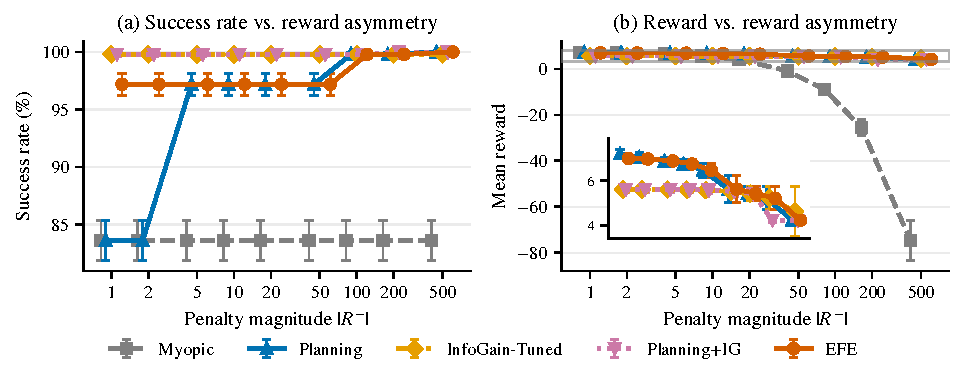
\includegraphics[width=\linewidth]{figures/fig_asymmetry_sweep.pdf}
\caption{Reward asymmetry sweep on Tiger ($H{=}6$, 500 episodes per point). EFE and Planning adapt smoothly across three orders of magnitude in penalty. Info Gain's fixed weight produces inconsistent performance.}
\label{fig:sweep}
\end{figure}

To test whether EFE's Tiger parity holds across reward scales, we sweep the penalty magnitude from $|R^-|{=}1$ to $500$. EFE naturally adapts its exploration depth, tracking the reward-optimal strategy without reconfiguration. Info Gain collapses at low penalties where its weight ($w{=}20$, tuned at $|R^-|{=}100$) drives excessive listening.

\section{Observation action scaling}
\label{app:obs_scaling}

\begin{figure}[h]
\centering
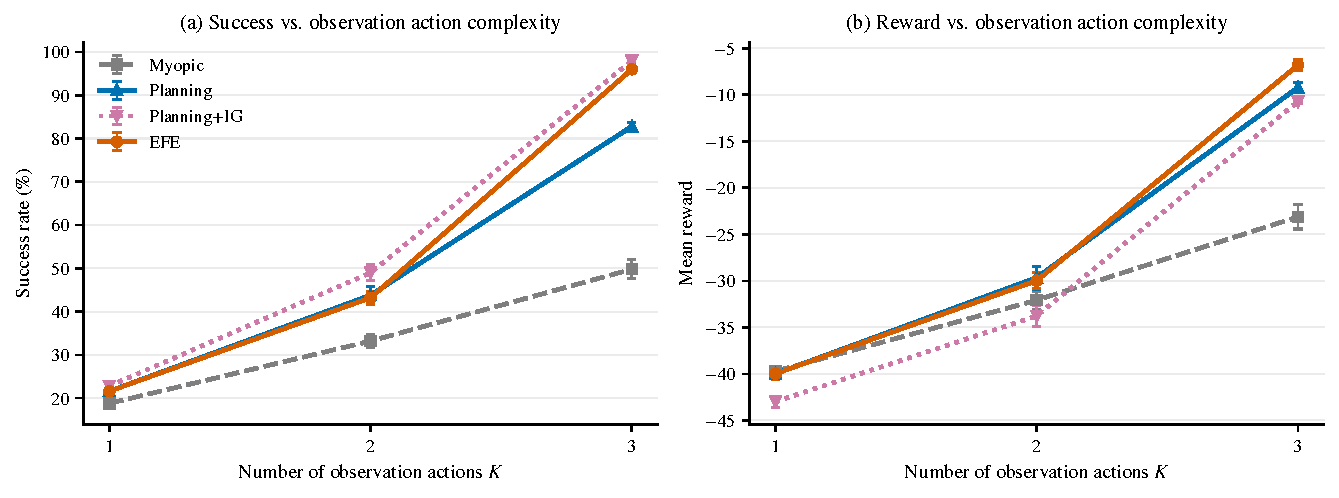
\includegraphics[width=\linewidth]{figures/fig_obs_scaling.pdf}
\caption{Observation action scaling on Diagnosis ($N{=}8$, $H{=}3$, 500 episodes). EFE's advantage over Planning grows with $K$, confirming that EFE is most valuable when the agent must choose among differentially informative observations.}
\label{fig:obs_scaling}
\end{figure}

Holding $N{=}8$ fixed on Diagnosis and varying $K$ from 1 to 3 isolates the ``which information'' hypothesis. At $K{=}1$, all agents face the same single test and perform similarly. As $K$ increases, EFE's advantage over Planning grows because the information gain term guides test selection.

\section{Tileworld belief evolution}
\label{app:tw_belief}

\begin{figure}[h]
\centering
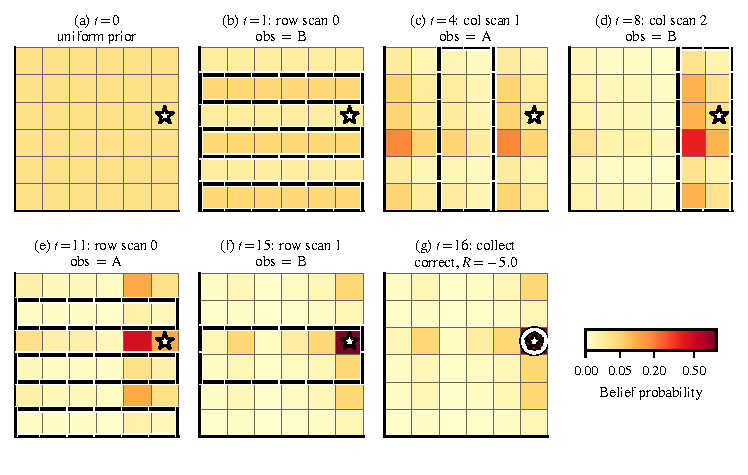
\includegraphics[width=\linewidth]{figures/fig_tileworld_belief.pdf}
\caption{Belief evolution within an EFE episode on the $6{\times}6$ Tileworld. Each panel shows belief probability over the 36 grid cells (darker = higher probability) after successive scans. Blue outlines mark the scanned region. The agent concentrates belief toward the target tile (green star) and commits once confident.}
\label{fig:tw_belief}
\end{figure}

\section{EFE trajectory decomposition}
\label{app:efe_trajectory}

\begin{figure}[h]
\centering
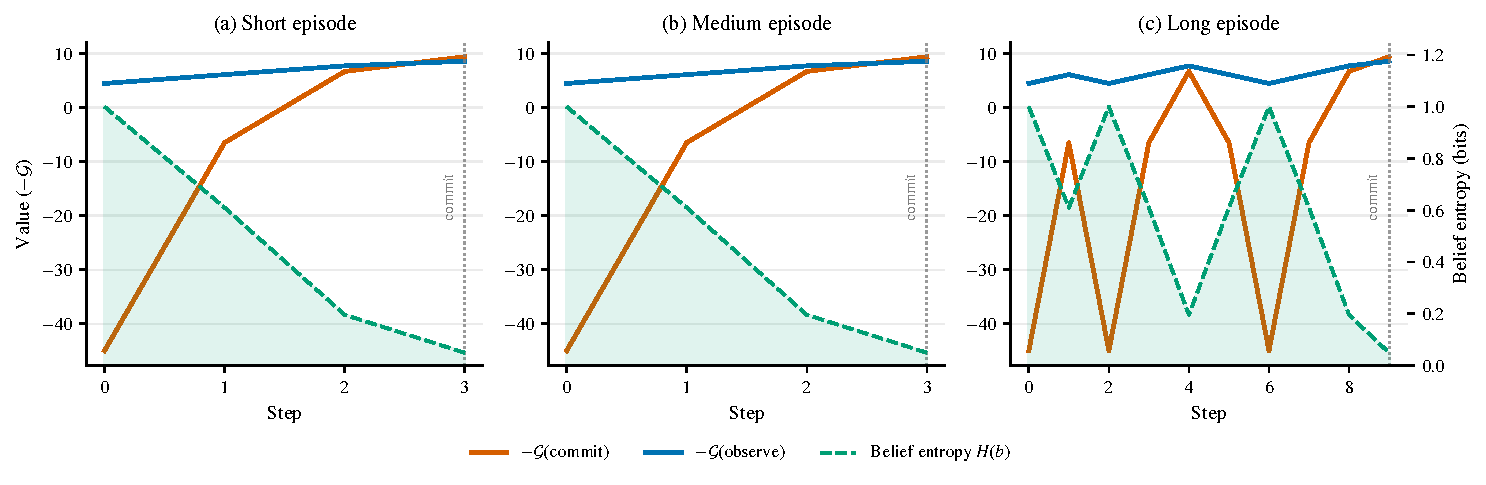
\includegraphics[width=\linewidth]{figures/fig_efe_trajectory.pdf}
\caption{EFE decomposition within Tiger episodes ($H{=}6$). The agent commits at the crossover where commit value (red) exceeds observe value (blue). As belief entropy (green shading) decreases, the transition from exploration to exploitation occurs automatically.}
\label{fig:traj}
\end{figure}

\section{Environment specifications}
\label{app:envs}

\begin{table}[h]
\centering
\caption{Full environment specifications.}
\begin{small}
\begin{tabular}{lccccccc}
\toprule
Environment & $|S|$ & Obs.\ actions & Commit actions & Accuracy & Obs.\ cost & Correct & Incorrect \\
\midrule
Tiger & 2 & 1 & 2 & 0.85 & $-1.0$ & $+10$ & $-100$ \\
Testbed & 2 & 1 & 2 & 0.75 & $-0.1$ & $+1$ & $-1$ \\
Diagnosis ($N{=}4$) & 4 & 2 & 4 & 0.80 & $-1.0$ & $+10$ & $-50$ \\
Bandit ($K{=}4$) & 4 & 4 & 4 & 0.80 & $-0.5$ & $+10$ & $+1$ \\
Navigation & 9 & 4 (move) & 0 (implicit) & var. & $-0.5$ & $+20$ & -- \\
Tileworld ($6{\times}6$) & 36 & 6 (scan) & 36 (collect) & 0.80 & $-1.0$ & $+10$ & $-50$ \\
\bottomrule
\end{tabular}
\end{small}
\end{table}

All environments are implemented as Gymnasium \citep{towers2024} environments with the standard \texttt{reset}/\texttt{step} API. The Diagnosis environment uses $K = \lceil \log_2 N \rceil$ binary tests, each providing noisy information about a different partition of the state space. The Navigation environment uses proximity-based warm/cold signals with accuracy depending on Manhattan distance to the hidden goal. The Tileworld projects the Diagnosis partition structure onto a 2D grid: $K = 2 \lceil \log_2 N \rceil$ scans partition the grid by bit-level splits of the row and column indices, enabling complete spatial disambiguation.

\section{Navigation results}
\label{app:navigation}

Navigation uses only move actions. The goal cell is hidden, and each move yields a proximity-based warm/cold observation (Section~\ref{app:envs}). Unlike Diagnosis or Tileworld, there is no separate menu of observation actions: information arrives as a side effect of translation, and greedy progress toward the belief mode already provides correlated evidence.

\begin{table}[h]
\centering
\caption{Navigation scaling ($150$ episodes per seed $\times$ $5$ seeds = $750$ episodes per agent per grid). Step budget $3n^2$. NavEFE uses depth-limited planning $H{=}2$. See \texttt{results\_navigation\_scaling.csv}.}
\label{tab:nav_scaling}
\begin{small}
\begin{tabular}{lcccc}
\toprule
Grid & $|S|$ & Agent & Success & Mean reward \\
\midrule
\multirow{3}{*}{$3{\times}3$} & \multirow{3}{*}{$9$} & NavMyopic & $90.4\%$ & $+2.04$ \\
& & NavInfoGain & $86.4\%$ & $-1.37$ \\
& & NavEFE ($H{=}2$) & $87.2\%$ & $-1.29$ \\
\midrule
\multirow{3}{*}{$5{\times}5$} & \multirow{3}{*}{$25$} & NavMyopic & $80.7\%$ & $-16.64$ \\
& & NavInfoGain & $76.0\%$ & $-23.24$ \\
& & NavEFE ($H{=}2$) & $74.4\%$ & $-25.76$ \\
\midrule
\multirow{3}{*}{$7{\times}7$} & \multirow{3}{*}{$49$} & NavMyopic & $65.7\%$ & $-38.42$ \\
& & NavInfoGain & $60.3\%$ & $-44.28$ \\
& & NavEFE ($H{=}2$) & $62.8\%$ & $-40.86$ \\
\bottomrule
\end{tabular}
\end{small}
\end{table}

NavMyopic (move toward the highest-probability cell) remains the strongest baseline at every scale: extra steps devoted to exploratory detours incur the per-move cost without the sharp information returns seen when tests can be chosen explicitly. This is not a failure of $w{=}1$ so much as a structural regime change relative to our main benchmarks. Importantly, NavEFE is competitive with one-step NavInfoGain at $7{\times}7$ (higher mean reward, comparable success), showing that recursive epistemic valuation is not harmful once the grid is large enough that myopic IG is already costly. The contrast with Tileworld (Figure~\ref{fig:tw_scaling}) underscores condition (1) in Section~\ref{sec:discussion}: EFE's clearest wins appear when the agent must select among differentially informative observation actions, not only where to translate next under a smooth proximity field.

\section{Scaling analysis}
\label{app:scaling}

\begin{table}[h]
\centering
\caption{Scaling analysis: Diagnosis $N = 2$ to $16$ (2{,}500 episodes: 500 per seed $\times$ 5 seeds, $H{=}2$).}
\begin{small}
\begin{tabular}{clccc}
\toprule
$N$ & Agent & Tests & Success & Reward \\
\midrule
\multirow{4}{*}{2}  & Myopic    & 1.00 & 80.3\% & $-2.83$ \\
                     & \textbf{Planning}  & \textbf{2.91} & \textbf{94.1\%} & $\mathbf{+3.56}$ \\
                     & Info Gain & 1.00 & 80.3\% & $-2.83$ \\
                     & \textbf{EFE} & \textbf{2.91} & \textbf{94.1\%} & $\mathbf{+3.56}$ \\
\midrule
\multirow{4}{*}{4}  & Myopic & 2.00 & 64.5\% & $-13.29$ \\
                     & \textbf{Planning} & \textbf{5.83} & \textbf{88.8\%} & $\mathbf{-2.58}$ \\
                     & Info Gain & 2.00 & 64.5\% & $-13.29$ \\
                     & \textbf{EFE} & \textbf{5.83} & \textbf{88.8\%} & $\mathbf{-2.58}$ \\
\midrule
\multirow{4}{*}{8}  & Myopic & 3.00 & 51.1\% & $-22.33$ \\
                     & Planning & 8.79 & 83.9\% & $-8.44$ \\
                     & Info Gain & 3.00 & 51.1\% & $-22.33$ \\
                     & \textbf{EFE} & \textbf{8.83} & \textbf{84.1\%} & $\mathbf{-8.38}$ \\
\midrule
\multirow{4}{*}{16} & Myopic & 4.00 & 40.8\% & $-29.50$ \\
                     & \textbf{Planning} & \textbf{11.65} & \textbf{77.4\%} & $\mathbf{-15.23}$ \\
                     & Info Gain & 4.00 & 40.8\% & $-29.50$ \\
                     & EFE & 11.64 & 77.1\% & $-15.37$ \\
\bottomrule
\end{tabular}
\end{small}
\end{table}

At $H{=}2$, EFE and Planning show no consistent gap at any $N$ tested here (bit-identical at $N{=}2$ and $N{=}4$; nominally within a point of each other at $N{=}8$ and $N{=}16$, with no consistent direction and no SE computed for this sweep), both substantially outperforming Myopic and untuned Info Gain. This contrasts with the $H{=}3$ Diagnosis result (Table~\ref{tab:main}), where EFE outperformed Planning by $+8.3$ pp, confirming that EFE's advantage requires sufficient recursive depth, not merely a larger state space. EFE-over-Myopic advantage grows from $+13.8$ pp at $N{=}2$ to $+36.3$ pp at $N{=}16$, confirming that deeper planning is increasingly valuable as state spaces grow, independent of whether EFE or reward-only Planning supplies that depth.

\section{PyMDP validation}
\label{app:pymdp}

We validated our EFE computation against the \texttt{pymdp} library \citep{heins2022} by wrapping pymdp's standard Agent class. Both implementations agree on observe-vs-commit decisions across all tested belief states (uniform, intermediate, and confident beliefs on the two-state environments). Information gain values computed by our recursive scheme and pymdp's \texttt{control} module agree qualitatively, with differences attributable to our recursive multi-step evaluation vs.\ pymdp's single-step policy enumeration.

\section{Epistemic foraging dynamics}
\label{app:foraging}

The aggregate statistics in Table~\ref{tab:main} show what EFE achieves. We now visualize how it achieves it by examining within-episode dynamics on extended Diagnosis instances ($N{=}8$, $K{=}3$, accuracy 0.75) that produce episodes with 8--15+ observation steps.

\paragraph{Belief evolution.}
Figure~\ref{fig:belief_heatmap} shows belief-state evolution within representative episodes for EFE, Planning, and Info Gain. EFE exhibits systematic partition-based narrowing: early tests eliminate large groups of states, and later tests refine among remaining candidates. Planning (without epistemic value) makes observations but lacks guidance on which test to run, producing less structured belief concentration. Info Gain continues testing well past the point where the agent has high confidence.

\begin{figure}[h]
\centering
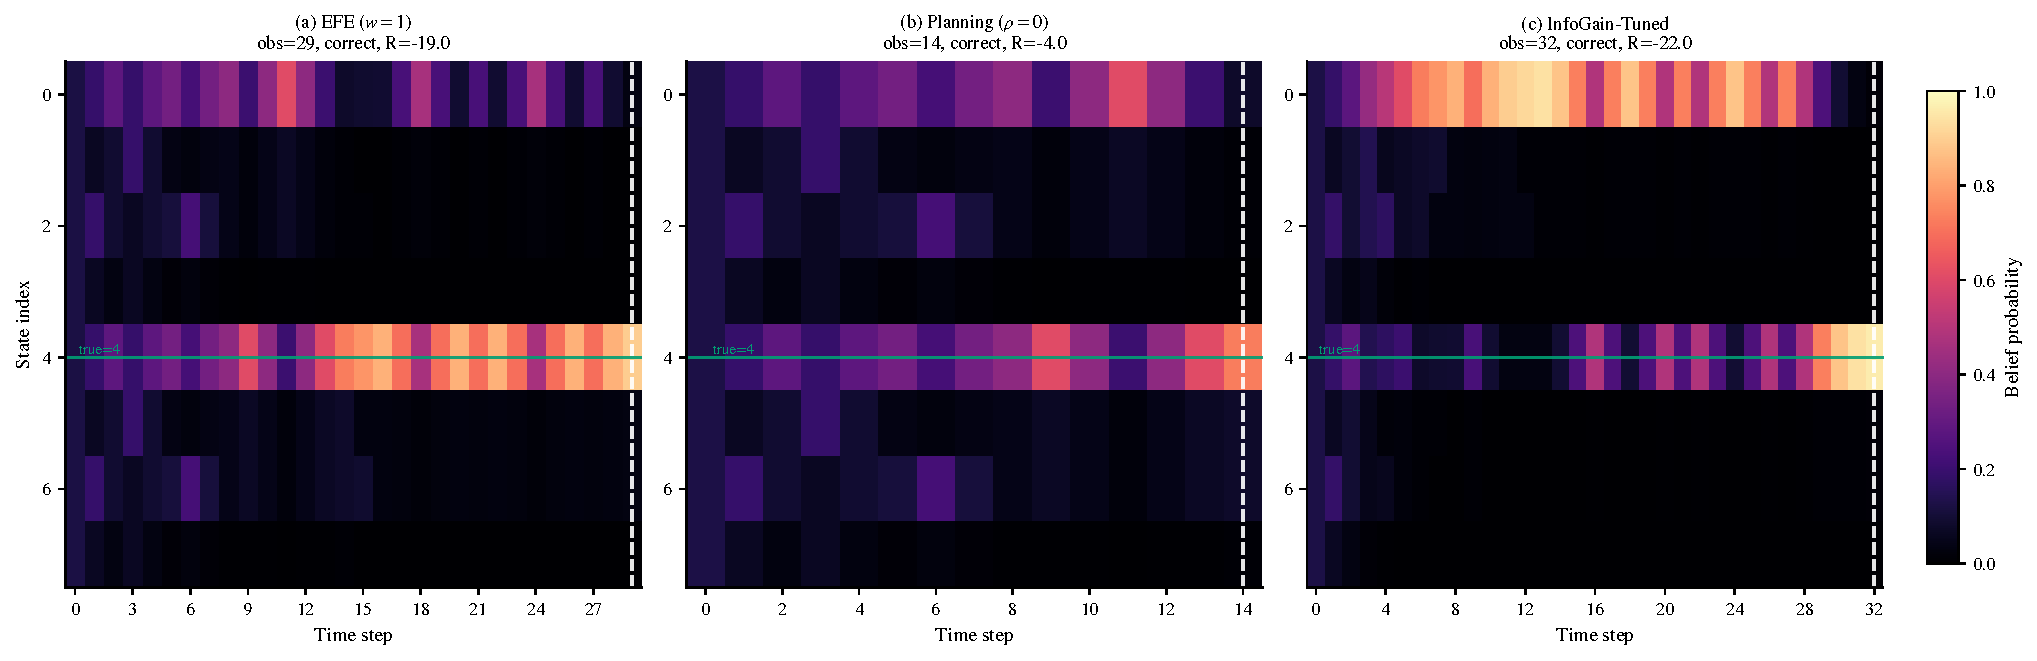
\includegraphics[width=\linewidth]{figures/fig_belief_heatmap.pdf}
\caption{Belief evolution within representative Diagnosis episodes ($N{=}8$, $K{=}3$, accuracy 0.75). Darker = higher probability. Green: true state. Dashed: commit point. EFE concentrates belief efficiently. Info Gain over-explores.}
\label{fig:belief_heatmap}
\end{figure}

\paragraph{Exploration efficiency.}
Figure~\ref{fig:efficiency} quantifies the temporal dynamics of epistemic foraging averaged across 300 episodes. EFE reduces entropy at a rate comparable to Planning+IG but commits earlier, avoiding the diminishing-returns regime. The ``survival curve'' of exploration shows EFE with a concentrated drop-off around steps 8--12, while Planning+IG's survival curve extends further right.

\begin{figure}[h]
\centering
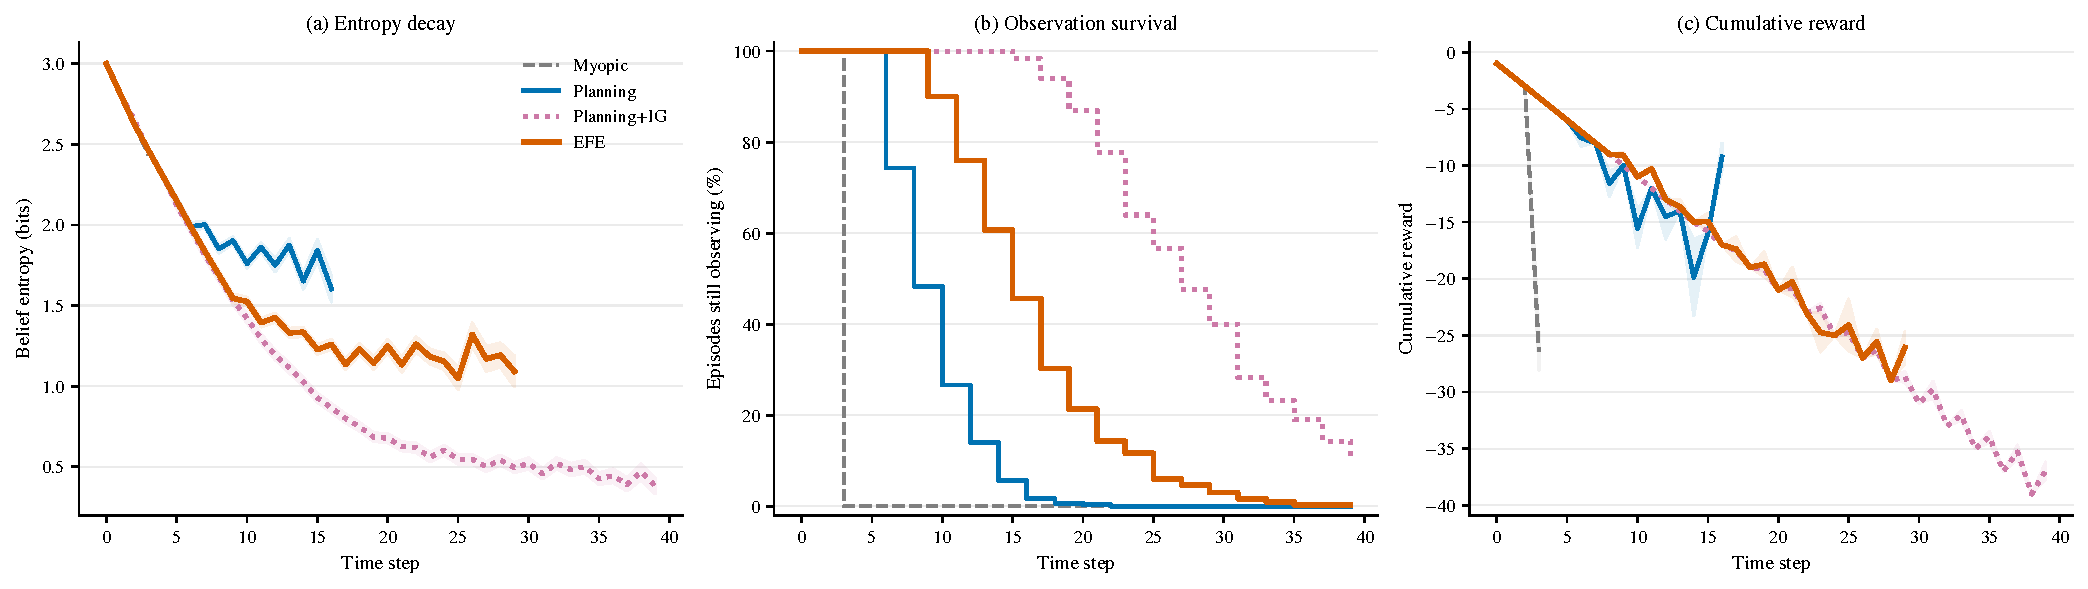
\includegraphics[width=\linewidth]{figures/fig_efficiency_curves.pdf}
\caption{Exploration efficiency on Diagnosis ($N{=}8$, $K{=}3$, 300 episodes). (a) Belief entropy decay. (b) Fraction of episodes still observing. (c) Cumulative reward. EFE commits at the right time. Planning+IG over-explores.}
\label{fig:efficiency}
\end{figure}

\section{Extended EFE decomposition}
\label{app:extended_efe}

\begin{figure}[h]
\centering
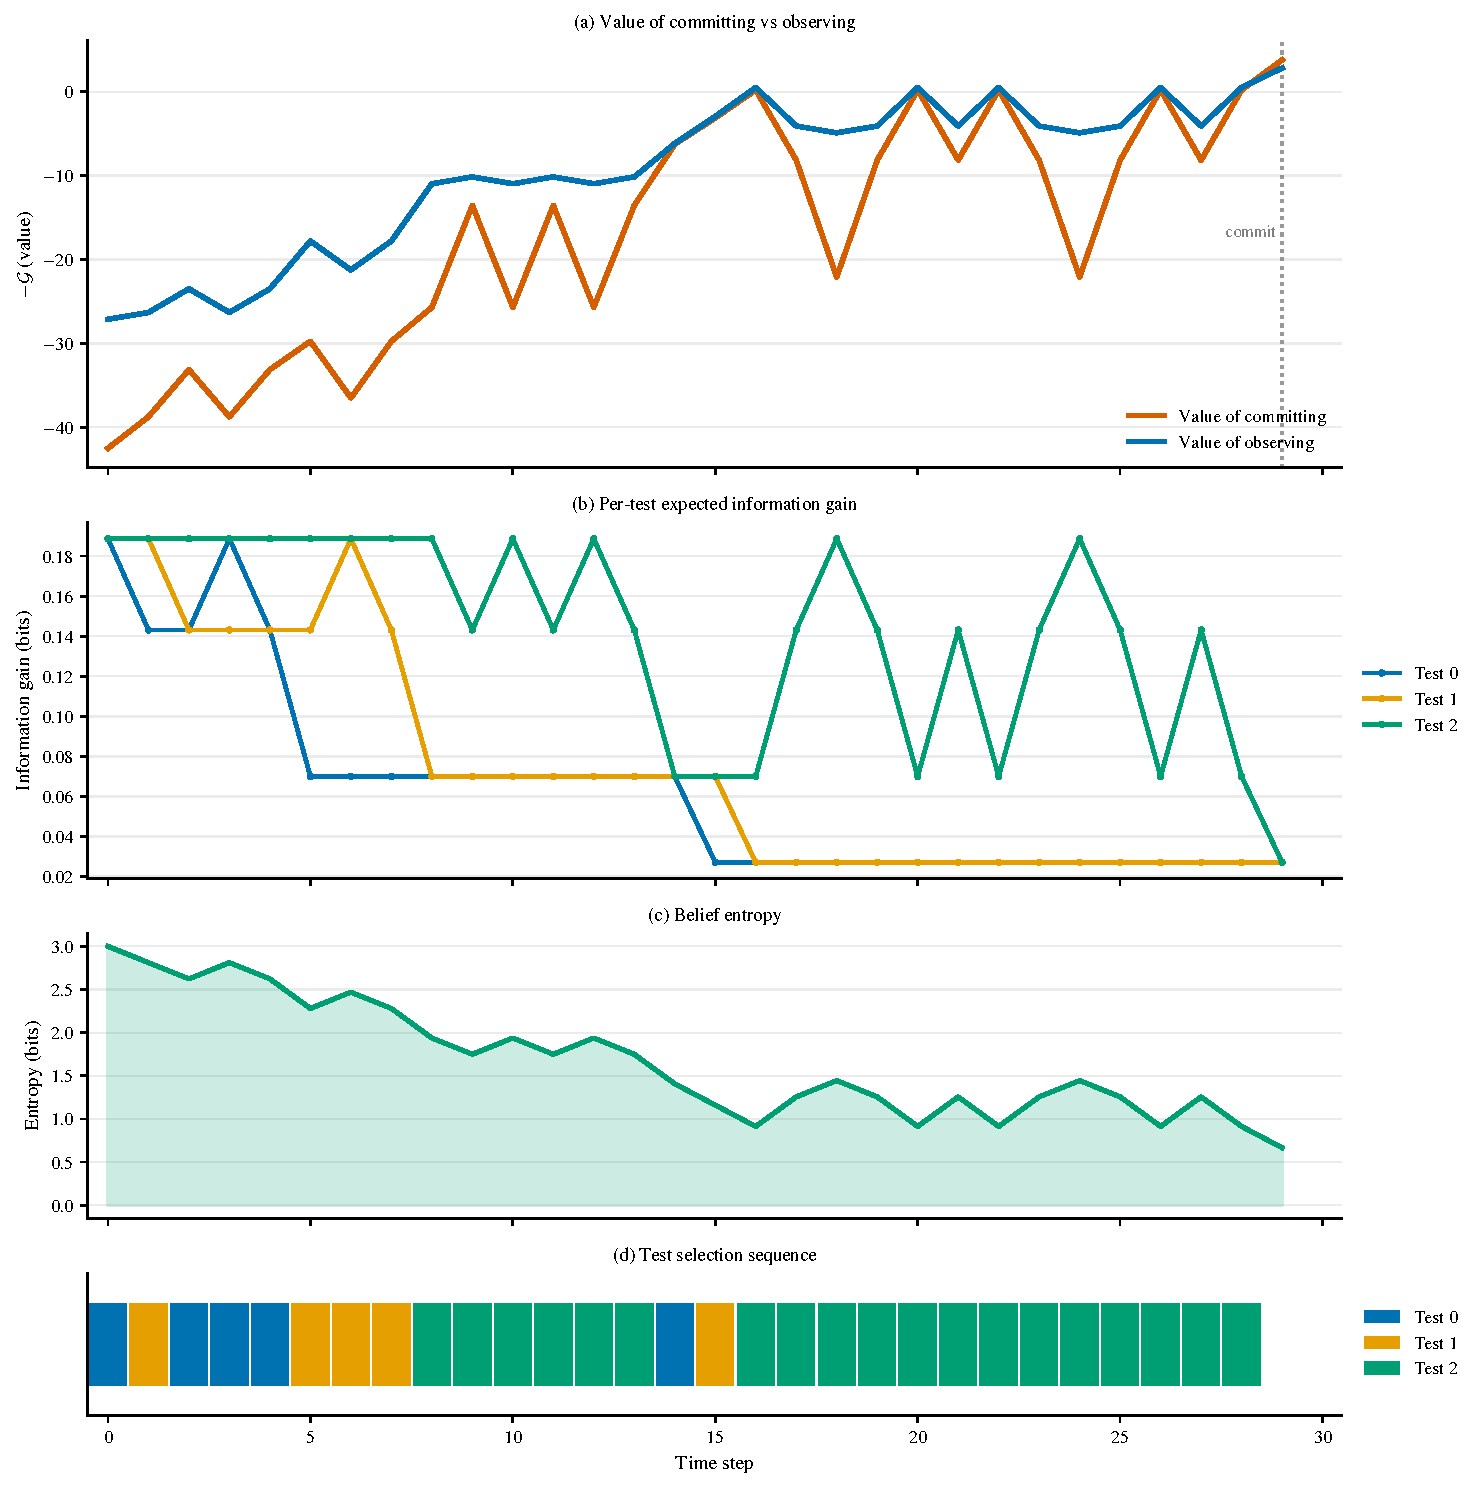
\includegraphics[width=\linewidth]{figures/fig_extended_efe.pdf}
\caption{EFE decomposition over an extended Diagnosis episode ($N{=}8$, $K{=}3$). (a)~Value of committing vs.\ observing, where the agent commits at the crossover. (b)~Per-test expected information gain: tests become differentially informative as belief concentrates, and the agent selects the most informative test at each step. (c)~Belief entropy decay. (d)~Test selection sequence showing the agent's adaptive strategy.}
\label{fig:extended_efe}
\end{figure}

Figure~\ref{fig:extended_efe} extends the EFE trajectory analysis of Figure~\ref{fig:traj} to a multi-observation-action environment where the agent must choose among $K{=}3$ diagnostic tests at each step. Panel (b) reveals a key dynamic: as the agent gathers information, the tests become differentially informative: some partitions of the state space become irrelevant once the agent has narrowed down the true condition, while others remain critical. The EFE agent tracks this structure, selecting the most informative available test at each step (panel d). This adaptive test selection is the mechanism underlying EFE's advantage over reward-only planning in multi-observation-action environments.

\section{Stopping time analysis}
\label{app:stopping}

\begin{figure}[h]
\centering
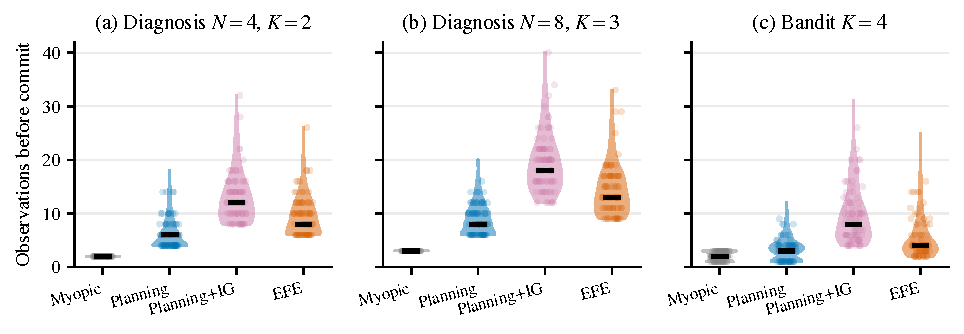
\includegraphics[width=\linewidth]{figures/fig_stopping_times.pdf}
\caption{Distribution of episode lengths (observation steps before commit) across agents and environments. Violin plots with overlaid data points. EFE exhibits concentrated stopping times, committing with consistent timing once sufficient confidence is reached. Planning commits earlier (sometimes prematurely), while Planning+IG over-explores with high variance.}
\label{fig:stopping}
\end{figure}

Figure~\ref{fig:stopping} shows the full distribution of stopping times (the number of observation steps each agent takes before committing) across three environment configurations. The shape of these distributions reveals qualitative differences in decision strategy: EFE's distributions are concentrated, indicating consistent and confident stopping behavior. Planning's distributions skew shorter, reflecting its tendency to commit before full disambiguation (especially visible on the $K{=}3$ Diagnosis environment). Planning+IG shows long right tails, confirming that the additive weight drives over-exploration with high variance. The EFE agent's concentrated stopping times are a consequence of the information-unit weight $w{=}1$: the crossover between observation and commit values occurs at a consistent belief-confidence level across episodes.

\section{Supplementary statistics}
\label{app:stats}

All pairwise comparisons use independent two-sample $t$-tests with Holm--Bonferroni correction for family-wise error control. Bootstrap 95\% confidence intervals use 10{,}000 resamples with fixed seed for reproducibility. Effect sizes use Cohen's $d$ with pooled standard deviation. Because episodes within a seed are not independent, we also report seed-level $t$-tests on per-seed means ($n{=}5$ seeds) and hierarchical bootstrap CIs that resample seeds then episodes within seed. The main-text table (Table~\ref{tab:main}) reports the seed-level SE as the primary uncertainty measure, since each answers a different question (episode-level precision versus between-seed replicability) and neither alone is a strict superset of the other; the full appendix tables below (Appendix~\ref{app:full_tables}) report the pooled episode-level SE only, for compactness across the full agent set, while the companion \texttt{*\_stats.csv} files committed alongside each battery's CSV carry the full seed-level Welch $t$-tests and Cohen's $d$ this section describes.

\begin{table}[h]
\centering
\caption{Cohen's $d$ for EFE vs.\ each baseline on mean episode reward (top) and success rate (bottom). Positive $d$ favors EFE. Interpretation: $|d|{<}0.2$ negligible, $0.2$--$0.5$ small, $0.5$--$0.8$ medium, $|d|{>}0.8$ large. Success-rate $d$ uses the same pooled-$s$ convention as reward (proportions treated as per-episode Bernoulli outcomes).}
\label{tab:effect_sizes}
\begin{small}
\begin{tabular}{llrl}
\toprule
Environment & Comparison & $d$ (reward) & Interpretation \\
\midrule
Tiger & EFE vs.\ Myopic & $+0.44$ & small \\
Tiger & EFE vs.\ Planning & $0.00$ & negligible (exact tie) \\
Tiger & EFE vs.\ Info Gain & $0.00$ & negligible (exact tie) \\
Tiger & EFE vs.\ Planning+IG & $+0.14$ & negligible \\
\midrule
Testbed & EFE vs.\ Myopic & $-0.03$ & negligible \\
Testbed & EFE vs.\ Planning & $-0.19$ & negligible \\
Testbed & EFE vs.\ Info Gain & $+1.34$ & large \\
Testbed & EFE vs.\ Planning+IG & $+1.33$ & large \\
\midrule
Diagnosis & EFE vs.\ Myopic & $+0.55$ & medium \\
Diagnosis & EFE vs.\ Planning & $+0.08$ & negligible \\
Diagnosis & EFE vs.\ Info Gain & $+0.25$ & small \\
Diagnosis & EFE vs.\ Planning+IG & $+0.25$ & small \\
\midrule
Bandit & EFE vs.\ Myopic & $+0.18$ & negligible \\
Bandit & EFE vs.\ Planning & $+0.14$ & negligible \\
Bandit & EFE vs.\ Info Gain & $+0.36$ & small \\
Bandit & EFE vs.\ Planning+IG & $+0.37$ & small \\
\midrule
\multicolumn{4}{l}{\textit{Success rate} ($d$ favors EFE)} \\
\midrule
Tiger & EFE vs.\ Planning & $0.00$ & negligible (exact tie) \\
Testbed & EFE vs.\ Planning & $+0.27$ & small \\
Diagnosis & EFE vs.\ Planning & $+0.33$ & small \\
Bandit & EFE vs.\ Planning & $+0.40$ & small \\
\bottomrule
\end{tabular}
\end{small}
\end{table}

The reward table shows that EFE vs.\ Planning is negligible to none on Tiger, Diagnosis, and Bandit (exactly zero on Tiger, where EFE and Planning tie): once both agents take enough informative actions, mean returns are similar, even though success rates differ. The success-rate rows isolate the axis where EFE improves most relative to Planning on Diagnosis and Bandit. Against over-exploring tuned alternatives (InfoGain-Tuned, Planning+IG), EFE shows large reward effects on the Testbed ($d > 1.3$) and small effects on Bandit ($d \approx 0.36$-$0.37$), reflecting the cost of over-exploration once Bandit's tuned weight is calibrated correctly ($w{=}20$, not the earlier mistuned $w{=}50$).

\section{Near-optimality across planning horizons}
\label{app:nearopt_horizon}

Proposition~\ref{prop:nearopt} bounds $w^*_{\mathrm{lo}}$ and $w^*_{\mathrm{hi}}$ for a single decision at $H{=}1$. To check whether the resulting near-optimality claim survives recursive multi-step planning, we generated 100 random two-state environments (reward asymmetry $\alpha \in [1,50]$, observation accuracy $p \in [0.55, 0.95]$, cost $\in [0.1, 5]$) and, for each environment and each $H \in \{1,2,3\}$, computed the reward-optimal weight $w^*$ by grid search and recorded whether $w{=}1$ falls within $\max(5\%, 0.5)$ of the best achievable reward. Figure~\ref{fig:nearopt_horizon} reports the fraction of environments where $w{=}1$ passes this test at each horizon, stratified by $\alpha$. The near-optimality rate rises from 30\% at $H{=}1$ to 58\% at $H{=}2$ and 79\% at $H{=}3$ (26\%~$\to$~53\%~$\to$~79\% restricted to $\alpha \geq 10$), so deeper planning widens the basin in which the untuned information-unit weight is reward-competitive rather than narrowing it. This is the same trend reported for Bandit in Section~\ref{sec:pareto}, where the low reward asymmetry predicts only marginal $H{=}1$ sufficiency yet multi-step EFE performs well in practice.

\begin{figure}[ht]
\centering
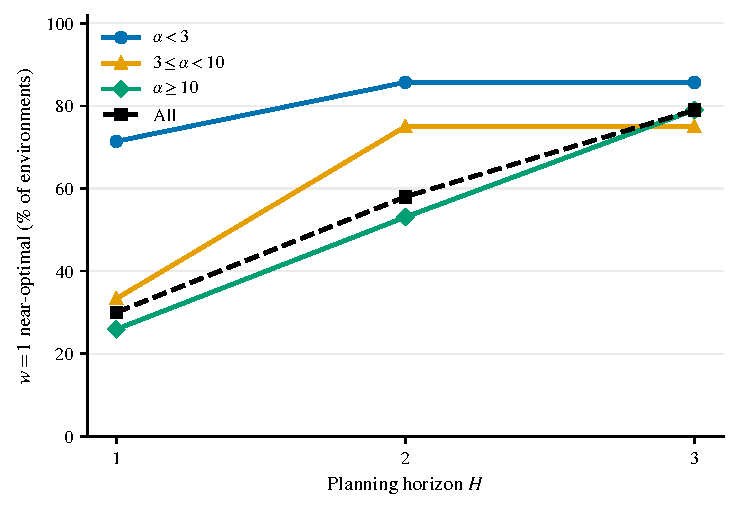
\includegraphics[width=0.7\linewidth]{figures/fig_nearopt_horizon.pdf}
\caption{Fraction of randomly generated two-state environments where $w{=}1$ is near-optimal, as a function of planning horizon $H$, stratified by reward asymmetry $\alpha$. The near-optimality basin widens with horizon, confirming that multi-step planning amplifies the value of observation. 100 environments, $\alpha \in [1,50]$, $p \in [0.55, 0.95]$, cost $\in [0.1, 5]$.}
\label{fig:nearopt_horizon}
\end{figure}

\paragraph{Horizon map: where myopic and deeper planning agree, and where they do not.} Figure~\ref{fig:nearopt_horizon} stratifies only by reward asymmetry $\alpha$. Table~\ref{tab:horizon-map} breaks the same 100 environments down by all three sampled regime axes and adds a direct per-environment comparison of the $H{=}1$ classification against $H{\geq}2$. Every regime axis shows the same qualitative pattern -- near-optimality is rarer at $H{=}1$ than at $H{=}3$ -- but the effect is sharpest for high-informativeness observations ($p \geq 0.85$: $17\% \to 90\%$) and comparatively flat for low reward asymmetry ($\alpha < 3$: already $71\%$ near-optimal at $H{=}1$, rising only to $86\%$ by $H{=}2$ and holding there through $H{=}3$, on 7 environments). The per-environment comparison shows the two horizons agree on 44 of the 100 environments: 30 agree $w{=}1$ is always near-optimal, 14 agree it never is, and the remaining 56 environments where $H{=}1$ predicts $w{=}1$ is \emph{not} near-optimal turn out to be near-optimal at some deeper horizon (myopic underclaiming -- the safe direction, a missed opportunity rather than a risk). On this random sample, zero environments show the opposite pattern (myopic overclaiming, where $H{=}1$ predicts near-optimality but a deeper horizon does not deliver it): every environment that passes the $H{=}1$ check also passes at $H{\geq}2$, so a practitioner validating $w{=}1$ with a cheap $H{=}1$ check on this environment family would not have been misled toward deploying it at a deeper horizon where it underperforms. This is a property of the observed sample, not a proven guarantee: we report it as an empirical boundary map over one random family of two-state environments, not an adaptive-submodularity result, and we make no claim that the $H{=}1$ check is monotone or that overclaiming is impossible in general, only that it did not occur here (the raw per-environment agreement data is in \texttt{results/results\_horizon\_map\_agreement.csv}, generated by \texttt{experiments/build\_horizon\_map.py}).

% Table auto-generated by experiments/build_horizon_map.py from
% results/results_nearopt_horizon.csv -- see that script to regenerate.
% Auto-generated by experiments/build_horizon_map.py -- do not edit by hand.
\begin{table}[t]
\centering
\caption{Horizon map: fraction of randomly generated two-state environments
 where $w{=}1$ is near-optimal (within $\max(5\%, 0.5)$ of the
 reward-optimal weight), stratified by each sampled regime axis and
 planning horizon $H$. Same 100 environments as Figure~\ref{fig:nearopt_horizon}
 (Appendix~\ref{app:nearopt_horizon}); this is an empirical boundary map, not an
 adaptive-submodularity guarantee.}
\label{tab:horizon-map}
\small
\begin{tabular}{lccc}
\toprule
Regime & $H{=}1$ & $H{=}2$ & $H{=}3$ \\
\midrule
\multicolumn{4}{l}{\textit{$\alpha$ (reward asymmetry)}} \\
\quad $\alpha<3$ & 0\% & 43\% & 29\% \\
\quad $3 \le \alpha < 10$ & 0\% & 25\% & 50\% \\
\quad $\alpha \ge 10$ & 14\% & 19\% & 37\% \\
\multicolumn{4}{l}{\textit{$p$ (observation informativeness)}} \\
\quad $p<0.65$ & 20\% & 8\% & 24\% \\
\quad $0.65 \le p < 0.85$ & 11\% & 9\% & 31\% \\
\quad $p \ge 0.85$ & 3\% & 50\% & 60\% \\
\multicolumn{4}{l}{\textit{cost (observation cost)}} \\
\quad cost$<1$ & 5\% & 16\% & 42\% \\
\quad $1 \le$ cost$<3$ & 5\% & 18\% & 37\% \\
\quad cost$\ge 3$ & 19\% & 26\% & 37\% \\
\bottomrule
\end{tabular}
\par\vspace{2pt}\footnotesize $H{=}1$ vs.\ $H{\geq}2$ agreement: 50\% of 100 environments agree; myopic overclaims 8, underclaims 42.
\end{table}


\section{Discount factor sensitivity}
\label{app:discount}

We test EFE and Planning agents' sensitivity to discounting by sweeping $\gamma \in \{0.9, 0.95, 0.99, 1.0\}$ across three environments, at the canonical 5-seed protocol. Including Planning at each $\gamma$ enables comparison of the relative gap between agents under discounting.

\begin{table}[h]
\centering
\caption{EFE and Planning agent performance across discount factors $\gamma$ (2{,}500 episodes: 500 per seed $\times$ 5 seeds -- lighter than Table~\ref{tab:main}'s 5{,}000-episode battery, so small numeric differences from that table on the $\gamma{=}1.0$ row are expected). $\Delta$Succ.\ shows the success rate gap (EFE $-$ Planning) at each $\gamma$, with the seed-level Welch $p$-value in parentheses; $^*$ marks significance after Holm--Bonferroni correction.}
\label{tab:discount}
\begin{small}
\begin{tabular}{llccccc}
\toprule
Environment & Agent & $\gamma$ & Obs. & Success & Reward & $\Delta$Succ. ($p$) \\
\midrule
\multirow{8}{*}{Tiger}
& EFE & 0.90 & 4.23 & 99.6\% & $+5.33$ & \multirow{2}{*}{$+2.7$ ($p<10^{-3}$)$^*$} \\
& Planning & 0.90 & 2.65 & 96.9\% & $+3.91$ & \\
& EFE & 0.95 & 4.23 & 99.6\% & $+5.33$ & \multirow{2}{*}{$0.0$ ($p{=}1.0$)} \\
& Planning & 0.95 & 4.23 & 99.6\% & $+5.33$ & \\
& EFE & 0.99 & 4.23 & 99.6\% & $+5.33$ & \multirow{2}{*}{$0.0$ ($p{=}1.0$)} \\
& Planning & 0.99 & 4.23 & 99.6\% & $+5.33$ & \\
& EFE & 1.00 & 4.23 & 99.6\% & $+5.33$ & \multirow{2}{*}{$0.0$ ($p{=}1.0$)} \\
& Planning & 1.00 & 4.23 & 99.6\% & $+5.33$ & \\
\midrule
\multirow{8}{*}{Diagnosis}
& EFE & 0.90 & 5.83 & 88.8\% & $-2.58$ & \multirow{2}{*}{$+0.0$ ($p{=}0.96$)} \\
& Planning & 0.90 & 5.86 & 88.7\% & $-2.62$ & \\
& EFE & 0.95 & 5.83 & 88.8\% & $-2.58$ & \multirow{2}{*}{$+0.0$ ($p{=}0.96$)} \\
& Planning & 0.95 & 5.86 & 88.7\% & $-2.62$ & \\
& EFE & 0.99 & 9.67 & 97.5\% & $-1.19$ & \multirow{2}{*}{$+7.9$ ($p<10^{-4}$)$^*$} \\
& Planning & 0.99 & 5.89 & 89.6\% & $-2.15$ & \\
& EFE & 1.00 & 9.68 & 97.4\% & $-1.26$ & \multirow{2}{*}{$+8.6$ ($p<10^{-4}$)$^*$} \\
& Planning & 1.00 & 5.85 & 88.8\% & $-2.59$ & \\
\midrule
\multirow{8}{*}{Bandit}
& EFE & 0.90 & 2.04 & 61.9\% & $+5.55$ & \multirow{2}{*}{$-0.2$ ($p{=}0.95$)} \\
& Planning & 0.90 & 2.04 & 62.0\% & $+5.56$ & \\
& EFE & 0.95 & 2.04 & 61.9\% & $+5.55$ & \multirow{2}{*}{$-0.2$ ($p{=}0.95$)} \\
& Planning & 0.95 & 2.04 & 62.0\% & $+5.56$ & \\
& EFE & 0.99 & 5.16 & 86.9\% & $+6.24$ & \multirow{2}{*}{$+22.4$ ($p<10^{-4}$)$^*$} \\
& Planning & 0.99 & 2.38 & 64.5\% & $+5.61$ & \\
& EFE & 1.00 & 5.16 & 86.9\% & $+6.24$ & \multirow{2}{*}{$+17.0$ ($p<10^{-4}$)$^*$} \\
& Planning & 1.00 & 3.24 & 69.9\% & $+5.67$ & \\
\bottomrule
\end{tabular}
\end{small}
\end{table}

\paragraph{Discounting erases EFE's advantage on multi-observation environments.} On Tiger (single observation action), both agents achieve ${\geq}96\%$ success across all $\gamma$ values, with a significant but small $+2.7$ pp EFE advantage at the heaviest discounting tested ($\gamma{=}0.9$, seed-level Welch $p<10^{-3}$); at $\gamma \geq 0.95$ the two agents are numerically identical ($p{=}1.0$). On Diagnosis and Bandit, heavy discounting ($\gamma{=}0.9$--$0.95$) renders both agents effectively myopic, erasing EFE's advantage entirely: at $\gamma{=}0.9$--$0.95$, EFE's epistemic term cannot propagate value through future observations because discounting truncates the effective horizon below the number of observations needed for disambiguation. Both agents observe the same number of times on Bandit (${\sim}2$) and Diagnosis (${\sim}6$) at these discount levels, and the residual success gaps are not statistically significant (Diagnosis diff $\approx 0.04$pp, $p{=}0.96$; Bandit diff $\approx -0.16$pp, $p{=}0.95$; Table~\ref{tab:discount}). The transition between $\gamma{=}0.95$ and $\gamma{=}0.99$ is sharp and, with 5-seed replication, clearly significant: at $\gamma{=}0.99$, EFE's success gap over Planning jumps to $+7.9$ pp on Diagnosis and $+22.4$ pp on Bandit (both $p<10^{-4}$), matching the undiscounted pattern ($+8.6$ pp Diagnosis, $+17.0$ pp Bandit at $\gamma{=}1.0$, both $p<10^{-4}$). This confirms that EFE's advantage depends on the discount factor preserving a sufficient effective horizon for recursive epistemic evaluation. In practical terms, $\gamma \geq 0.99$ is needed for EFE to differentiate from reward-only planning on these environments, and the 5-seed replication makes this a statistically confirmed threshold rather than a single-seed point estimate.

\section{Model misspecification sensitivity}
\label{app:misspec}

Our main results assume the agent's generative model matches the true environment dynamics. Here we investigate robustness when the agent's believed observation accuracy $p_{\text{agent}}$ differs from the true accuracy $p_{\text{true}}$, creating a systematic model mismatch.

\begin{table}[h]
\centering
\caption{Model misspecification on Tiger ($p_{\text{true}}{=}0.85$, $H{=}4$, 2{,}500 episodes across 5 seeds -- lighter than Table~\ref{tab:main}'s 5{,}000-episode battery, so small numeric differences from that table's calibrated row are expected). The mismatch column shows $p_{\text{agent}} - p_{\text{true}}$.}
\label{tab:misspec-tiger}
\begin{small}
\begin{tabular}{llcccc}
\toprule
Agent & $p_{\text{agent}}$ & Mismatch & Obs & Success & Reward \\
\midrule
EFE & 0.70 & $-0.15$ & 4.23 & 99.6\% & $+5.33$ \\
EFE & 0.75 & $-0.10$ & 4.23 & 99.6\% & $+5.33$ \\
EFE & 0.80 & $-0.05$ & 4.23 & 99.6\% & $+5.33$ \\
EFE & 0.85 & $\pm 0.00$ & 4.23 & 99.6\% & $+5.33$ \\
EFE & 0.90 & $+0.05$ & 2.65 & 96.9\% & $+3.91$ \\
EFE & 0.95 & $+0.10$ & 2.65 & 96.9\% & $+3.91$ \\
\midrule
Planning & 0.70 & $-0.15$ & 4.23 & 99.6\% & $+5.33$ \\
Planning & 0.85 & $\pm 0.00$ & 4.23 & 99.6\% & $+5.33$ \\
Planning & 0.95 & $+0.10$ & 2.65 & 96.9\% & $+3.91$ \\
\bottomrule
\end{tabular}
\end{small}
\end{table}

\begin{table}[h]
\centering
\caption{Model misspecification on Diagnosis ($p_{\text{true}}{=}0.80$, $H{=}3$, 2{,}500 episodes across 5 seeds).}
\label{tab:misspec-diag}
\begin{small}
\begin{tabular}{llcccc}
\toprule
Agent & $p_{\text{agent}}$ & Mismatch & Obs & Success & Reward \\
\midrule
EFE & 0.65 & $-0.15$ & 5.86 & 88.7\% & $-2.62$ \\
EFE & 0.70 & $-0.10$ & 9.68 & 97.4\% & $-1.26$ \\
EFE & 0.75 & $-0.05$ & 9.68 & 97.4\% & $-1.26$ \\
EFE & 0.80 & $\pm 0.00$ & 9.68 & 97.4\% & $-1.26$ \\
EFE & 0.85 & $+0.05$ & 5.86 & 88.7\% & $-2.62$ \\
EFE & 0.90 & $+0.10$ & 5.86 & 88.7\% & $-2.62$ \\
\midrule
Planning & 0.65 & $-0.15$ & 5.84 & 89.2\% & $-2.35$ \\
Planning & 0.80 & $\pm 0.00$ & 5.85 & 88.8\% & $-2.59$ \\
Planning & 0.90 & $+0.10$ & 5.82 & 88.7\% & $-2.61$ \\
\bottomrule
\end{tabular}
\end{small}
\end{table}

\paragraph{Key findings.} On Tiger, both EFE and Planning agents are remarkably robust: success rates remain above 96.9\% even with $\pm 0.15$ mismatch. The degradation pattern is asymmetric but not in observation count: negative mismatch (underestimating accuracy, including exact calibration) leaves observation count and success unchanged (4.23 observations, 99.6\% success at every level from $-0.15$ to $0.00$), whereas positive mismatch (overestimating accuracy) sharply reduces observation count (to 2.65) and lowers success to 96.9\%. Under the fixed pipeline, EFE and Planning give numerically identical rows at every mismatch level tested on Tiger (Table~\ref{tab:misspec-tiger}): with a single observation action, the belief-update dynamics driven by the agent's believed accuracy determine when committing becomes attractive, and information gain has no separate observation action to redirect toward, so there is no EFE-specific buffering effect to report here. This is a genuine, environment-specific finding, not a case we can attribute to the epistemic term: the same asymmetric degradation appears in reward-only Planning, which has no information-gain term at all.

On Diagnosis, EFE's behavior steps between exactly two levels rather than degrading smoothly with mismatch magnitude (Table~\ref{tab:misspec-diag}): a high-testing level (9.68 observations, 97.4\% success) at mismatch $\in \{-0.10, -0.05, 0.00\}$, and a low-testing level (5.86 observations, 88.7\% success) at mismatch $\in \{-0.15, +0.05, +0.10\}$. This is not the ``well-calibrated agent tests most, both directions of error reduce testing'' pattern reported previously: perfect calibration ($\pm 0.00$) ties with two levels of underestimation rather than uniquely maximizing testing, and only the most extreme underestimate tested ($-0.15$) drops to the low-testing level, matching every overestimate we tested. Overestimating accuracy (the agent believes tests are more informative than they truly are) makes each test look more decisive than it is, so the agent commits prematurely on insufficient evidence and lands in the low-testing, lower-success regime at every overestimate level tested. Underestimating accuracy makes each test look less informative than it is, but only past a threshold: mild underestimation ($-0.05$, $-0.10$) does not visibly change behavior from perfect calibration, while severe underestimation ($-0.15$) triggers the same reduced-testing response as overestimation, producing a similar-looking success rate (88.7\%) that is, as before, driven by fewer rather than more observations. Reward-only Planning shows a comparable but not identical step pattern (Table~\ref{tab:misspec-diag}), so this threshold structure is not unique to EFE's epistemic term; we do not have a mechanistic account of why the transition sits precisely where it does and report the pattern descriptively rather than explain it.

\paragraph{Implications for learned models.} These results suggest that EFE-based agents can tolerate moderate model errors without catastrophic failure. In practice, observation models learned from data will have estimation error. The graceful degradation observed here indicates that approximate models suffice for effective EFE-driven information gathering, provided the model does not systematically overestimate sensor informativeness.

\section{Interleaved observe-act: RockSample (extended)}
\label{app:rocksample}

This appendix provides extended RockSample results beyond the main text (Section~\ref{sec:rocksample}), including a POMCP(1000) baseline on every instance, the full Planning+IG sweep ($w{=}5, 10$), and per-instance step and check counts. All numbers below are read directly from the same CSVs as Table~\ref{tab:rocksample} (\texttt{results\_rocksample\_\{5x3,7x4,7x8,11x11\}.csv}), regenerated by \texttt{experiments/build\_rocksample\_tables.py}; no numbers in this appendix are computed separately from the main table.

% Auto-generated by experiments/build_rocksample_tables.py -- do not edit by hand.
\begin{table}[ht]
\centering
\caption{RockSample extended results: full agent roster including
 a POMCP(1000) baseline on every instance and Planning+IG at
 both $w{=}5$ and $w{=}10$. Steps and checks are episode means.
 RS[5,3]/RS[7,4]: 500 episodes $\times$ 10 seeds. RS[7,8]/RS[11,11]:
 100 episodes $\times$ 5 seeds.}
\label{tab:rocksample_extended}
\begin{small}
\begin{tabular}{llccccc}
\toprule
Instance & Agent & Steps & Checks & Good & Bad & Reward \\
\midrule
\multirow{6}{*}{RS[5,3]}
 & Greedy & $12.00$ & $0.00$ & $1.49$ & $1.51$ & $+3.71 \pm 0.25$ \\
 & POMCP (1000) & $51.00$ & $20.69$ & $1.22$ & $0.03$ & $-9.92 \pm 0.19$ \\
 & Planning (d=3) & $10.38$ & $3.71$ & $0.99$ & $0.04$ & $+14.28 \pm 0.11$ \\
 & Plan+IG w=5 (d=3) & $15.81$ & $5.36$ & $1.44$ & $0.01$ & $+16.41 \pm 0.11$ \\
 & Plan+IG w=10 (d=3) & $20.35$ & $6.63$ & $1.48$ & $0.00$ & $+14.60 \pm 0.11$ \\
 & EFE w=1 (d=3) & $15.26$ & $4.79$ & $1.44$ & $0.03$ & $+16.47 \pm 0.12$ \\
\midrule
\multirow{6}{*}{RS[7,4]}
 & Greedy & $22.00$ & $0.00$ & $1.98$ & $2.02$ & $-1.38 \pm 0.29$ \\
 & POMCP (1000) & $85.97$ & $41.05$ & $1.58$ & $0.04$ & $-25.51 \pm 0.21$ \\
 & Planning (d=4) & $10.00$ & $2.00$ & $0.95$ & $0.05$ & $+13.97 \pm 0.11$ \\
 & Plan+IG w=5 (d=4) & $24.55$ & $8.15$ & $1.69$ & $0.01$ & $+14.56 \pm 0.12$ \\
 & Plan+IG w=10 (d=4) & $26.82$ & $8.80$ & $1.78$ & $0.01$ & $+14.27 \pm 0.12$ \\
 & EFE w=1 (d=4) & $16.81$ & $5.36$ & $1.44$ & $0.01$ & $+15.96 \pm 0.12$ \\
\midrule
\multirow{6}{*}{RS[7,8]}
 & Greedy & $32.00$ & $0.00$ & $4.02$ & $3.98$ & $-5.60 \pm 1.23$ \\
 & POMCP (1000) & $129.00$ & $82.43$ & $1.51$ & $0.05$ & $-49.90 \pm 0.46$ \\
 & Planning (d=3) & $4.51$ & $1.00$ & $0.48$ & $0.03$ & $+12.31 \pm 0.24$ \\
 & Plan+IG w=5 (d=3) & $40.27$ & $14.19$ & $3.40$ & $0.01$ & $+23.76 \pm 0.51$ \\
 & Plan+IG w=10 (d=3) & $57.47$ & $18.26$ & $3.94$ & $0.01$ & $+20.55 \pm 0.51$ \\
 & EFE w=1 (d=3) & $27.26$ & $9.84$ & $2.61$ & $0.06$ & $+21.85 \pm 0.53$ \\
\midrule
\multirow{6}{*}{RS[11,11]}
 & Greedy & $57.00$ & $0.00$ & $5.48$ & $5.52$ & $-18.90 \pm 1.45$ \\
 & POMCP (1000) & $231.00$ & $165.75$ & $2.98$ & $0.16$ & $-87.22 \pm 0.61$ \\
 & Planning (d=2) & $2.50$ & $1.00$ & $0.48$ & $0.03$ & $+13.23 \pm 0.24$ \\
 & Plan+IG w=5 (d=2) & $3.09$ & $1.56$ & $0.50$ & $0.03$ & $+13.18 \pm 0.25$ \\
 & Plan+IG w=10 (d=2) & $3.09$ & $1.56$ & $0.50$ & $0.03$ & $+13.18 \pm 0.25$ \\
 & EFE w=1 (d=2) & $2.50$ & $1.00$ & $0.48$ & $0.03$ & $+13.23 \pm 0.24$ \\
\bottomrule
\end{tabular}
\end{small}
\end{table}


The Greedy agent moves to rocks and samples them without checking quality first, incurring frequent bad-rock penalties (1.51--3.98 across instances). EFE moves toward uncertain rocks, checks them to resolve quality, then samples selectively, so bad samples stay low (0.01--0.06) on RS[5,3], RS[7,4], and RS[7,8]; RS[11,11] is the exception where all informed agents (including Planning at $w{=}0$) converge to the same low-activity policy, discussed in Section~\ref{sec:rocksample}. POMCP collapses to a large negative reward on every instance ($-9.92$ to $-87.22$), the same directed-checking gap already documented in Appendix~\ref{app:pomcp}.

Planning+IG at $w{=}5$ and $w{=}10$ lets us check whether $w{=}1$ leaves performance on the table when a higher weight is allowed. On RS[5,3], $w{=}5$ is not significantly different from EFE ($w{=}1$) ($+16.41$ vs.\ $+16.47$, seed-level Welch $p{=}0.74$), while $w{=}10$ is significantly worse ($+14.60$ vs.\ $+16.47$, $p<10^{-8}$), so nothing is gained by tuning beyond $w{=}1$ here, and pushing the weight too far past it actively hurts. On RS[7,4], EFE ($w{=}1$) outright beats both tuned weights ($+15.96$ vs.\ $+14.56$ and $+14.27$, both $p<10^{-5}$): more checking here (Plan+IG's higher check counts) does not translate into more good rocks sampled, so the untuned weight is better calibrated on this instance. On RS[7,8], the pattern is neither monotone in the weight nor a simple case of ``more checking helps'': $w{=}5$ (+23.76) and EFE (+21.85) are not significantly different ($p{=}0.09$ after correction), while $w{=}10$ (+20.55) is significantly worse than $w{=}5$ ($p{=}0.003$), so the intermediate tuned weight is at worst tied with the untuned $w{=}1$ and reliably beats the more aggressive $w{=}10$, whose extra checking (57.47 steps, 18.26 checks per episode, versus $w{=}5$'s 40.27/14.19) costs more in observation spend than it recovers in avoided bad samples. The honest summary is that $w{=}1$ is not uniformly best on RockSample, and neither is any fixed direction of ``tune the weight higher'': $w{=}1$ wins outright on RS[7,4], and is not significantly different from the best tuned weight (never significantly beaten) on RS[5,3] and RS[7,8], where an even larger weight is significantly worse still. We report this rather than only the instances, or the tuning direction, where a simple story holds.

These results exercise the extension Proposition~\ref{prop:factored} already establishes for interleaved settings despite the transition--observation coupling analyzed in Section~\ref{sec:methodology} (factored observation extension). The agent's behavior mirrors the observe-then-commit pattern: check (gather information), then sample/exit (commit), even though checking and acting are interleaved with movement.

\section{IDS baseline (observe-then-commit)}
\label{app:ids}

We adapt information-directed sampling \citep{russo2014} to the observe-then-commit setting by minimizing the information ratio $\Delta^2/I$ over observation actions, where $\Delta$ is the opportunity cost of observing versus committing now and $I$ is expected information gain about the optimal commit. Table~\ref{tab:ids} reports a matched comparison (2{,}500 episodes: 500 per seed $\times$ 5 seeds, the canonical protocol) against Myopic, Planning, success-tuned Planning+IG, and EFE.

\begin{table}[h]
\centering
\caption{IDS vs.\ baselines (2{,}500 episodes: 500 per seed $\times$ 5 seeds -- lighter than Table~\ref{tab:main}'s 5{,}000-episode battery, so small numeric differences from that table's EFE/Planning rows are expected). IDS is competitive on Tiger (tying every other agent exactly there) but over-explores on Diagnosis and Bandit relative to EFE's untuned $w{=}1$, resembling success-tuned Planning+IG on reward.}
\label{tab:ids}
\begin{small}
\begin{tabular}{llccc}
\toprule
Environment & Agent & Obs. & Success & Reward \\
\midrule
\multirow{5}{*}{Tiger}
& Myopic & $1.00$ & 84.6\% & $-7.90$ \\
& Planning & $4.23$ & 99.6\% & $+5.33$ \\
& Planning+IG ($w{=}20$) & $4.23$ & 99.6\% & $+5.33$ \\
& EFE & $4.23$ & 99.6\% & $+5.33$ \\
& IDS & $4.23$ & 99.6\% & $+5.33$ \\
\midrule
\multirow{5}{*}{Diagnosis}
& Myopic & $2.00$ & 64.5\% & $-13.29$ \\
& Planning & $5.85$ & 88.8\% & $-2.59$ \\
& Planning+IG ($w{=}100$) & $13.17$ & 99.2\% & $-3.68$ \\
& EFE & $9.68$ & 97.4\% & $-1.26$ \\
& IDS & $13.17$ & 99.2\% & $-3.63$ \\
\midrule
\multirow{5}{*}{Bandit}
& Myopic & $2.05$ & 61.6\% & $+5.52$ \\
& Planning & $3.24$ & 69.9\% & $+5.67$ \\
& Planning+IG ($w{=}100$) & $12.36$ & 99.8\% & $+3.81$ \\
& EFE & $5.16$ & 86.9\% & $+6.24$ \\
& IDS & $10.62$ & 99.5\% & $+4.65$ \\
\bottomrule
\end{tabular}
\end{small}
\end{table}

On multi-observation environments, IDS reaches near-ceiling success but at a reward cost similar to success-tuned Planning+IG, whereas EFE ($w{=}1$) retains higher mean reward. The adaptive information ratio does not eliminate the need for a stopping trade-off calibrated to the reward scale; under our shared reward convention, the fixed information-unit weight remains the stronger untuned default for expected reward.

\section{Proper-scoring calibration}
\label{app:calibration}

The reward and success-rate metrics used throughout this paper score decisions, not beliefs. To check that the epistemic term is doing more than inflating a task-performance proxy, we separately score the terminal belief itself against the true hidden state using two proper scoring rules \citep{gneiting2007}: the log score ($\log b(s^\star)$, the same functional the epistemic value term is derived from) and the Brier score ($\sum_s (b(s) - \mathbb{1}[s=s^\star])^2$). A well-calibrated agent should not merely act correctly more often; its posterior should also assign more mass, in expectation, to the state that turns out to be true. Table~\ref{tab:calibration} reports mean $\pm$ SE over 5 seeds for Planning (reward-only), EFE ($w{=}1$), and a reference near-optimal or IG-heavy policy on the three core OTC environments plus both Structural Inspection instances (500 episodes per seed for Tiger, Diagnosis, Bandit, and Inspection-N8; 200 per seed for Inspection-N16): the point-based near-optimal solver SARSOP \citep{kurniawati2008}, run on a self-built alpha-vector policy evaluated in-simulator, for the three OTC environments where its belief is small enough to reach near-optimal convergence in reasonable time, and Planning+IG at the Stage G atlas's higher canonical budget for Structural Inspection, whose state space exceeds what our SARSOP build solves in reasonable time.

% Auto-generated by experiments/run_calibration_table.py -- do not edit by hand.
\begin{table}[t]
\centering
\caption{Proper-scoring calibration of the terminal belief against the
 true hidden state (log score in nats, Brier score; mean $\pm$ SE over
 5 seeds). Reference is SARSOP for the three OTC environments and
 Planning+IG at the Stage G atlas's higher canonical budget for
 Structural Inspection, where the near-optimal solver used here does not
 scale to the instance's state space.}
\label{tab:calibration}
\small
\begin{tabular}{llcc}
\toprule
Instance & Agent & Log score & Brier score \\
\midrule
Tiger & Planning (reward-only) & $-0.035 \pm 0.006$ & $0.011 \pm 0.002$ \\
Tiger & EFE (w=1) & $-0.035 \pm 0.006$ & $0.011 \pm 0.002$ \\
Tiger & SARSOP & $-0.035 \pm 0.006$ & $0.011 \pm 0.002$ \\
\midrule
Diagnosis & Planning (reward-only) & $-0.433 \pm 0.018$ & $0.199 \pm 0.011$ \\
Diagnosis & EFE (w=1) & $-0.134 \pm 0.004$ & $0.049 \pm 0.002$ \\
Diagnosis & SARSOP & $-0.154 \pm 0.021$ & $0.058 \pm 0.010$ \\
\midrule
Bandit & Planning (reward-only) & $-0.901 \pm 0.033$ & $0.463 \pm 0.019$ \\
Bandit & EFE (w=1) & $-0.525 \pm 0.027$ & $0.240 \pm 0.016$ \\
Bandit & SARSOP & $-0.510 \pm 0.034$ & $0.231 \pm 0.018$ \\
\midrule
Inspection-N8 & Planning (reward-only) & $-0.417 \pm 0.004$ & $0.286 \pm 0.003$ \\
Inspection-N8 & EFE (w=1) & $-0.245 \pm 0.004$ & $0.144 \pm 0.003$ \\
Inspection-N8 & Planning+IG (w=100) & $-0.008 \pm 0.001$ & $0.002 \pm 0.000$ \\
\midrule
Inspection-N16 & Planning (reward-only) & $-0.382 \pm 0.005$ & $0.251 \pm 0.003$ \\
Inspection-N16 & EFE (w=1) & $-0.257 \pm 0.003$ & $0.150 \pm 0.002$ \\
Inspection-N16 & Planning+IG (w=23.7) & $-0.032 \pm 0.004$ & $0.010 \pm 0.001$ \\
\bottomrule
\end{tabular}
\end{table}


Planning (reward-only) is calibration-dominated by every epistemic-aware agent on every instance except Tiger, where its single observation action already suffices and all three agents converge to the same policy and hence the same terminal belief. On Diagnosis, Bandit, and both Inspection instances, EFE's terminal belief scores substantially better under both rules than reward-only Planning's, and on the three OTC environments EFE ($w{=}1$) lies within overlapping SE bands of SARSOP's near-optimal calibration. This is evidence that the epistemic term produces genuinely better-informed terminal beliefs, not only better terminal actions; the two need not coincide, since an agent can commit correctly from a confidently wrong belief on environments with few reachable outcomes.

\section{Per-test value-of-information audit trail}
\label{app:audit}

Section~\ref{sec:discussion} argues that the epistemic value term supports interpretable decisions, but nothing in the main results exposes that decomposition directly. We add an optional, backward-compatible audit record at the shared Planning+IG evaluation boundary used by \texttt{PlanningInfoGainAgent}, \texttt{EFEAgent} (at $w{=}1$), and \texttt{InspectionTreeSearchAgent}: for every candidate action considered at the root of the decision, the record stores the sensing cost, the expected information gain in bits, the weighted information gain $w \cdot \mathrm{IG}$, the expected task value, and the resulting total score, plus which action was selected. Enabling this record does not change any action selection; it is a read-only projection of quantities the agent already computes, and unit tests confirm that the recorded total score always ranks the chosen action first and that its components sum correctly.

Table~\ref{tab:audit-case-study} shows one representative decision point from a Structural Inspection-N8 episode ($w{=}5$) where the ranking by total score disagrees with the ranking by raw information gain: \texttt{test1} carries almost 5$\times$ the information gain of \texttt{test0}, yet the agent selects \texttt{test0} because its higher sensing cost is not offset by a compensating gain in expected task value. This is the audit trail's purpose: it lets a practitioner check, for any single decision, whether an unexpected action was chosen for an information-theoretic reason or a task-value reason, rather than only reporting an aggregate reward or success rate. We keep this as an interpretability appendix artifact; it does not change any reported headline result.

% Auto-generated by experiments/run_audit_case_study.py -- do not edit by hand.
\begin{table}[t]
\centering
\caption{Per-action value-of-information audit for one representative decision
 (Inspection-N8, info-gain weight $w=5$, step 2 of the
 episode seeded at 42). Total score is the maximized planning
 objective (Section 6); the chosen action need not have the largest raw information
 gain once sensing cost and downstream task value are accounted for.}
\label{tab:audit-case-study}
\small
\begin{tabular}{lccccc}
\toprule
Action & Cost & IG (bits) & $w \cdot$IG & Task value & Total score \\
\midrule
test0 & 0.50 & 0.021 & 0.106 & -26.29 & -26.18 \\ % chosen
test1 & 2.00 & 0.106 & 0.528 & -26.87 & -26.34 \\
diagnose(nominal) & 0.00 & 0.000 & 0.000 & -26.86 & -26.86 \\
diagnose(faulty) & 0.00 & 0.000 & 0.000 & -31.05 & -31.05 \\
\bottomrule
\end{tabular}
\end{table}


\section{Reward-rescaling invariance}
\label{app:reward_scaling}

To test the scale objection directly, we multiply all rewards and costs by $k \in \{0.1, 1, 10\}$ on Diagnosis and Bandit and re-sweep Planning+IG weights. Maximizing $\mathbb{E}[kR] + w\,I$ matches the unscaled policy at weight $w'{=}kw$, so $w^*_{\mathrm{ret}}(k) \approx k\, w^*_{\mathrm{ret}}(1)$; equivalently, keeping $w$ fixed while scaling rewards by $k$ is indistinguishable from rescaling the weight by $1/k$. Figure~\ref{fig:reward_scaling} and Table~\ref{tab:reward_scaling} report the sweep (200 episodes $\times$ 3 seeds per $(k,w)$ pair). Results confirm covariance of $w^*_{\mathrm{ret}}$ with $k$: $w{=}1$ is not scale-invariant, and the paper's near-optimality claims are conditional on the shared reward convention used throughout the suite.

\begin{figure}[h]
\centering
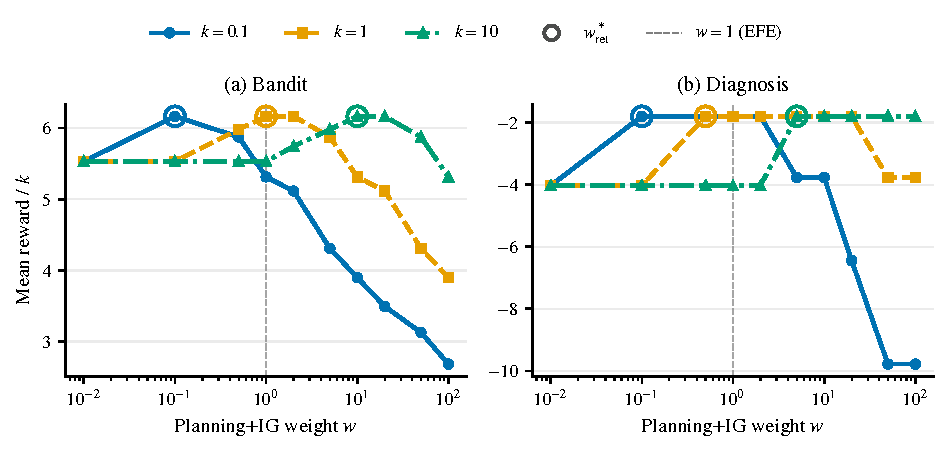
\includegraphics[width=0.95\linewidth]{figures/fig_reward_scaling.pdf}
\caption{Reward rescaling: mean reward vs.\ Planning+IG weight $w$ under global scale factors $k$. Stars mark $w^*_{\mathrm{ret}}$. The optimum shifts toward larger $w$ as $k$ grows, consistent with $w^*_{\mathrm{ret}}(k) \propto k$.}
\label{fig:reward_scaling}
\end{figure}

\begin{table}[h]
\centering
\caption{Reward-optimal Planning+IG weight under reward scale $k$. The direction of covariance is as predicted (larger scales favor larger weights). On Bandit the ratio $w^*_{\mathrm{ret}}/k$ is exactly constant across the three tested scales under the fixed pipeline; on Diagnosis it varies twofold (flat high-$w$ plateaus mean several grid weights tie for $w^*_{\mathrm{ret}}$, and ties are broken toward the smallest weight reaching the maximum), so the table is qualitative evidence of covariance on Diagnosis and a tight quantitative match on Bandit, not a precise stability estimate on this finite grid.}
\label{tab:reward_scaling}
\begin{small}
\begin{tabular}{lccc}
\toprule
Environment & $k$ & $w^*_{\mathrm{ret}}$ & $w^*_{\mathrm{ret}}/k$ \\
\midrule
Diagnosis & $0.1$ & $0.1$ & $1.0$ \\
Diagnosis & $1.0$ & $0.5$ & $0.5$ \\
Diagnosis & $10.0$ & $5.0$ & $0.5$ \\
Bandit & $0.1$ & $0.1$ & $1.0$ \\
Bandit & $1.0$ & $1.0$ & $1.0$ \\
Bandit & $10.0$ & $10.0$ & $1.0$ \\
\bottomrule
\end{tabular}
\end{small}
\end{table}

\section{POMCP baseline comparison}
\label{app:pomcp}

We compare against POMCP \citep{silver2010}, a standard online POMDP solver that handles exploration through Monte Carlo tree search with UCB1 action selection. This addresses whether EFE's explicit information gain valuation provides benefit over the implicit exploration in POMCP's tree search. Our implementation uses particle-based belief representation at each tree node, adapted to the observe-then-commit action structure. Crucially, our POMCP rollout policy is semi-informed: observation actions are selected uniformly at random, but the rollout terminates (stochastically, with 30\% probability per step) with a belief-optimal commit, i.e., the commit action maximizing expected reward under the Bayesian-updated rollout belief. This is strictly stronger than a fully random rollout, which would also randomize over commit actions. Each of the five outer seeds now initializes both the environment stream and the planner's internal random stream (particle sampling and rollouts) from that seed, so the reported variability reflects genuine run-to-run differences rather than a fixed planner seed obscuring one axis of variation; an earlier draft used a single fixed internal seed for the planner across all runs, which we have since corrected. The remaining gap between POMCP and EFE therefore reflects the value of observation selection: EFE chooses which test to run based on information gain, while POMCP samples tests uniformly. We sweep POMCP simulation budgets across $\{500, 1000, 2000, 5000\}$ and report wall-clock timings for a simulation-budget scaling analysis: the comparison is simulation-matched, not compute-matched, the same distinction drawn for the MCTS-EFE comparison above. Tree-node action selection uses UCB1 with exploration constant $10.0$ (\texttt{rho\_aif/agents/pomcp.py}), fixed across all environments; this was not tuned per environment, and because reward scales differ across our benchmarks (Section~\ref{sec:experiments}), the same exploration constant implies a different effective exploration--exploitation balance on each one, a caveat symmetric to the reward-scale sensitivity we report for $w$ (Section~\ref{sec:pareto}).

\begin{table}[h]
\centering
\caption{POMCP comparison config (5{,}000 total episodes across 5 per-run seeds $\{42,123,456,789,1024\}$ for Tiger/Diagnosis/Bandit and 1{,}000 for Tileworld; not the main-table protocol, and EFE/Planning here are run inside the POMCP harness rather than sourced from Table~\ref{tab:main}, so small differences from that table are expected). POMCP uses 1{,}000 simulations per decision. Reward: mean $\pm$ seed-level SE.}
\label{tab:pomcp}
\begin{small}
\begin{tabular}{llccc}
\toprule
Environment & Agent & Obs. & Success & Reward \\
\midrule
\multirow{3}{*}{Tiger} & \textbf{Planning} & $\mathbf{4.20}$ & $\mathbf{99.4\%}$ & $\mathbf{+5.19 \pm 0.21}$ \\
& POMCP (1000) & $1.80$ & 89.4\% & $-3.48 \pm 0.28$ \\
& \textbf{EFE} & $\mathbf{4.20}$ & $\mathbf{99.4\%}$ & $\mathbf{+5.19 \pm 0.21}$ \\
\midrule
\multirow{3}{*}{Diagnosis} & Planning & $5.86$ & 88.8\% & $-2.57 \pm 0.20$ \\
& POMCP (1000) & $3.96$ & 74.1\% & $-9.49 \pm 0.22$ \\
& \textbf{EFE} & $\mathbf{9.66}$ & $\mathbf{97.2\%}$ & $\mathbf{-1.37 \pm 0.18}$ \\
\midrule
\multirow{3}{*}{Bandit} & Planning & $3.29$ & 71.0\% & $+5.75 \pm 0.08$ \\
& POMCP (1000) & $7.20$ & 87.7\% & $+5.29 \pm 0.04$ \\
& \textbf{EFE} & $\mathbf{5.11}$ & $\mathbf{86.9\%}$ & $\mathbf{+6.27 \pm 0.04}$ \\
\midrule
\multirow{3}{*}{\shortstack[l]{Tileworld\\[-1pt]{\scriptsize $6{\times}6$}}} & Planning & -- & 73.6\% & $-21.41 \pm 0.64$ \\
& POMCP (1000) & -- & 5.6\% & $-47.99 \pm 0.72$ \\
& \textbf{EFE} & -- & $\mathbf{71.9\%}$ & $\mathbf{-21.62 \pm 0.87}$ \\
\bottomrule
\end{tabular}
\end{small}
\end{table}

\paragraph{Key findings.} POMCP underperforms both EFE and Planning on reward on every environment, and underperforms on success rate everywhere except Bandit, where it is now much closer to EFE than under the earlier fixed-planner-seed protocol. On Tiger, POMCP commits prematurely (1.80 observations vs.\ 4.20 for EFE), yielding 89.4\% success against EFE's 99.4\% (here numerically identical to Planning, per the exact tie documented in Section~\ref{sec:results}). On Diagnosis, the gap is dramatic: POMCP achieves only 74.1\% success ($-9.49$ reward) while EFE reaches 97.2\% ($-1.37$ reward). POMCP's random rollout policy cannot evaluate which of the $K{=}2$ diagnostic tests to run. It treats all observation actions equally, whereas EFE's information gain term directly values differential informativeness. On Bandit, POMCP's Monte Carlo exploration achieves a slightly higher success rate than EFE ($87.7 \pm 0.5\%$ vs.\ $86.9 \pm 0.3\%$ seed-level SE, $+0.8$ pp) but at real reward cost ($+5.29 \pm 0.04$ vs.\ EFE's $+6.27 \pm 0.04$): 7.20 inspections vs.\ EFE's 5.11. This is a smaller success-rate gap than the earlier fixed-planner-seed run suggested (which showed POMCP at 96.8\% vs.\ EFE's 89.0\%, a $+7.8$ pp gap, reported before per-run seeding was implemented and without a seed-level SE); with per-run seeding the two are close on success and EFE is still ahead on reward. On Tileworld ($6{\times}6$, $|S|{=}36$), POMCP collapses to 5.6\% success, as the 36 commit actions and 6 scan actions create a branching factor that overwhelms 1{,}000 simulations.

\paragraph{Simulation-budget scaling.} Increasing POMCP's simulation budget to 5{,}000 does not qualitatively change the picture: on Diagnosis, POMCP(5000) reaches $75.5 \pm 0.6\%$ success (seed-level SE), still far short of EFE's $97.2 \pm 0.3\%$, while taking substantially more wall-clock time per decision (547.2 ms/ep vs.\ EFE's closed-form computation). On Tiger, POMCP(5000) reaches $90.3 \pm 0.3\%$ but at roughly 5$\times$ the compute of the 1{,}000-simulation budget. On Bandit, POMCP(5000) reaches $97.2 \pm 0.2\%$ success (now clearly ahead of EFE) but its reward falls to $+5.18 \pm 0.04$ from $+5.29 \pm 0.04$ at 1{,}000 simulations and its wall-clock cost balloons to roughly 1.07 s/episode, a $\sim$5$\times$ slowdown versus the 1{,}000-simulation budget for a small reward decrease; this is the clearest case in our results of buying success-rate with both compute and return. These results indicate that EFE's advantage is not merely a compute-budget artifact but reflects the benefit of closed-form information gain valuation over Monte Carlo exploration \emph{as configured here} -- with this rollout policy and a single untuned exploration constant -- particularly on multi-observation-action environments where the agent must choose which information to gather. A stronger POMCP configuration (tuned exploration constants per reward scale, informed rollouts, or a reference implementation) could narrow the gap, and we do not claim the comparison bounds what a best-practice POMCP can achieve.

\paragraph{MCTS-EFE.} To disentangle EFE's information valuation from the planning mechanism, we implement MCTS-EFE: MCTS with EFE as the leaf heuristic rather than random rollouts, using UCB1 tree selection with max-backup value propagation and exact per-node information gain as the observe-action reward, so the tree optimizes the same objective as exact EFE rather than a proxy. On Tiger at $H{=}10$, MCTS-EFE with 500 simulations achieves 97.7\% success ($\approx$5.9s per 200 episodes), compared to POMCP's 88.8\% at the same simulation count ($\approx$4.1s; simulation-matched, not compute-matched) and exact EFE's 99.9\% at $H{=}6$ ($\approx$14.1s). In this configuration, EFE provides a stronger leaf evaluation function: the same MCTS framework with EFE leaf evaluation substantially outperforms semi-informed rollouts. On Tiger, MCTS-EFE's success and observation count are insensitive to both horizon (6, 8, 10) and simulation budget (200, 500, 1{,}000) in this range, saturating at 97.7\% success and 3.735 observations throughout; this reflects Tiger's small reachable-belief set, which the tree already covers well within 200 simulations, rather than the horizon or budget parameters having no effect in general.

\section{Budgeted $\rho$-POMDP supplementary details}
\label{app:budget_supp}

\subsection{SARSOP build and export details}
\label{app:sarsop_build}

Section~\ref{sec:sarsop}'s reference solver is the original APPL C++ toolkit (\texttt{pomdpsol}), built from source by \url{tools/build_sarsop.sh} with four documented patches required for a modern clang toolchain on Apple Silicon: dropping unsupported \texttt{-msse2} and \texttt{-mfpmath=sse} flags, replacing raw-pointer \texttt{SparseCol} iterators (modern libc++ cannot construct \texttt{std::vector::const\_iterator} from a raw pointer), converting chained comparison assertions to conjunctions, and suppressing implicit-function-declaration errors in the legacy Cassandra parser. The resulting binary is not committed; the patch script is. \url{experiments/run_sarsop_baseline.py} exports any discrete observe-then-commit benchmark generically from the same hidden-state, action-layout, and observation-model definitions the agents already use (an absorbing done state, discount $\gamma{=}0.999$), solves to precision $10^{-3}$, parses the resulting alpha-vector policy from its XML output, and evaluates it through the same episode runner used for every other agent so that mechanics and metrics are shared exactly. Four unit tests (\url{tests/test_sarsop_export.py}) cover the exporter, the policy parser, and the alpha-vector argmax agent without requiring the compiled binary, so the export pipeline is checked even in environments where the solver is unavailable.

\subsection{Distractor-diagnosis environment: factorization guarantee}
\label{app:distractor}

Section~\ref{sec:distractor}'s \texttt{DistractorDiagnosisEnv} joint state space is the product of a $4$-way condition and a binary nuisance factor. Every observation model in the environment (condition tests, the distractor test, and the terminal commit reward) is constructed to depend on exactly one of the two factors, so for a belief that itself factors as a product of independent condition and nuisance marginals, observing the distractor test updates the nuisance marginal and leaves the condition marginal exactly unchanged, and symmetrically for condition tests and the nuisance marginal. This is verified by $13$ unit tests (\url{tests/test_distractor_diagnosis.py}), including a direct check that the condition-marginal KL divergence before and after a distractor observation is exactly zero (up to floating-point tolerance) when the prior belief is factored, and a symmetric check for condition tests against the nuisance marginal. The guarantee is stated for factored beliefs specifically; a belief with residual condition--nuisance correlation (which does not arise under this environment's independent generative process, but could under model misspecification) is outside the scope of the proof.

\subsection{The $w^*$ atlas}
\label{app:w_atlas}

Table~\ref{tab:w-atlas} aggregates the usage-curve range, implicit EFE budget $B_{\mathrm{EFE}} = U(w{=}1)$, and two canonical-budget crossing brackets (Definition~\ref{def:pi3}) for every benchmark instance appearing in this paper, generated by \url{experiments/run_w_atlas.py} from the saved usage-curve CSVs of Sections~\ref{sec:results} and~\ref{sec:budget_experiments}. Brackets are set-valued by construction; the table implies no closed-form relationship between $B_{\mathrm{EFE}}$ and environment parameters such as reward scale, state count, or horizon, and none should be inferred from it.

% Table auto-generated by experiments/run_w_atlas.py from
% results/results_w_atlas.csv -- see that script to regenerate.
% Auto-generated by experiments/run_w_atlas.py -- do not edit by hand.
\begin{table}[t]
\centering
\caption{Atlas of operational sensing budgets across benchmark instances:
 usage range of the Planning+IG family, implicit EFE budget
 $B_{\mathrm{EFE}} = U(w{=}1)$ (mean $\pm$ SE over seeds), and crossing
 brackets $w^*(B)$ at two canonical budgets per instance. Brackets are
 set-valued (Definition PI-3); no closed-form meta-model is implied.}
\label{tab:w-atlas}
\small
\begin{tabular}{lcccc}
\toprule
Instance & $[U_{\min}, U_{\max}]$ & $B_{\mathrm{EFE}}$ & $B_1$: $w^*$ bracket & $B_2$: $w^*$ bracket \\
\midrule
Bandit & $[3.06, 12.20]$ & $5.03 \pm 0.17$ & 4.4: $(0.0611, 0.139]$ & 10.8: $(19.3, 43.9]$ \\
Diagnosis & $[5.72, 13.57]$ & $9.68 \pm 0.15$ & 6.9: $(0.139, 0.316]$ & 12.4: $(19.3, 43.9]$ \\
Inspection-N16 & $[22.42, 46.04]$ & $33.46 \pm 0.19$ & 26.0: $(0.316, 1.33]$ & 42.5: $(5.62, 23.7]$ \\
Inspection-N8 & $[12.65, 30.89]$ & $18.24 \pm 0.19$ & 15.4: $(0.316, 2.15]$ & 28.2: $(14.7, 100]$ \\
RS{[}5,3{]} & $[3.81, 9.10]$ & $4.90 \pm 0.08$ & 4.6: $(0.316, 1.33]$ & 8.3: $(23.7, 100]$ \\
RS{[}7,4{]} & $[2.00, 14.73]$ & $5.49 \pm 0.14$ & 3.9: $(0.316, 2.15]$ & 12.8: $(14.7, 100]$ \\
Tiger & $[3.98, 5.62]$ & $4.21 \pm 0.07$ & -- & 5.4: $(19.3, 43.9]$ \\
Tileworld-6x6 & $[14.92, 33.70]$ & $14.83 \pm 0.22$ & 17.7: $(5.62, 23.7]$ & 30.9: $(23.7, 100]$ \\
\bottomrule
\end{tabular}
\end{table}


\end{document}
